\documentclass[11pt]{article}

\usepackage[portuguese]{babel}
\usepackage[utf8]{inputenc}
\usepackage{amsmath}
\usepackage{graphicx}
\usepackage{float}
\usepackage{subfig}
\usepackage{fixltx2e}
\usepackage[bottom]{footmisc}
\usepackage{listings}
\usepackage{color} 
\usepackage{xargs}                      % Use more than one optional parameter in a new commands
\usepackage[pdftex,dvipsnames]{xcolor}  % Coloured text etc.
\usepackage[colorinlistoftodos,prependcaption,textsize=tiny]{todonotes}
\newcommandx{\unsure}[2][1=]{\todo[linecolor=red,backgroundcolor=red!25,bordercolor=red,#1]{#2}}
\newcommandx{\change}[2][1=]{\todo[linecolor=blue,backgroundcolor=blue!25,bordercolor=blue,#1]{#2}}
\newcommandx{\info}[2][1=]{\todo[linecolor=OliveGreen,backgroundcolor=OliveGreen!25,bordercolor=OliveGreen,#1]{#2}}
\newcommandx{\improvement}[2][1=]{\todo[linecolor=Plum,backgroundcolor=Plum!25,bordercolor=Plum,#1]{#2}}
\newcommandx{\thiswillnotshow}[2][1=]{\todo[disable,#1]{#2}}
\usepackage[font=footnotesize]{caption}

\definecolor{keywordcolor}{rgb}{0,0.4,0.7}
\definecolor{commentcolor}{rgb}{0.4,0.4,0.4} 	
\definecolor{mygray}{rgb}{0.5,0.5,0.5} 	% line counter color
\definecolor{mymauve}{rgb}{0.90,0.25,0.47}	% string color
\definecolor{codebackground}{rgb}{0.95,0.95,0.95} 

\lstset{ %
	backgroundcolor=\color{codebackground},   % choose the background color; you must add \usepackage{color} or \usepackage{xcolor}
	basicstyle=\ttfamily \footnotesize,        % the size of the fonts that are used for the code
	breakatwhitespace=false,         % sets if automatic breaks should only happen at whitespace
	breaklines=true,                 % sets automatic line breaking
	captionpos=b,                    % sets the caption-position to bottom
	commentstyle=\color{commentcolor},    % comment style
	deletekeywords={...},            % if you want to delete keywords from the given language
	escapeinside={\%*}{*)},          % if you want to add LaTeX within your code
	extendedchars=true,              % lets you use non-ASCII characters; for 8-bits encodings only, does not work with UTF-8
	keepspaces=true,                 % keeps spaces in text, useful for keeping indentation of code (possibly needs columns=flexible)
	keywordstyle=\color{keywordcolor},       % keyword style
	numbers=left,                    % where to put the line-numbers; possible values are (none, left, right)
	numbersep=5pt,                   % how far the line-numbers are from the code
	numberstyle=\tiny\color{mygray}, % the style that is used for the line-numbers
	rulecolor=\color{black},         % if not set, the frame-color may be changed on line-breaks within not-black text (e.g. comments (green here))
	showspaces=false,                % show spaces everywhere adding particular underscores; it overrides 'showstringspaces'
	showstringspaces=false,          % underline spaces within strings only
	showtabs=false,                  % show tabs within strings adding particular underscores
	stepnumber=1,                    % the step between two line-numbers. If it's 1, each line will be numbered
	%stringstyle=\color{mymauve},     % string literal style
	  identifierstyle=\color{mymauve},
	tabsize=2                       % sets default tabsize to 2 spaces
}

\setcounter{tocdepth}{1}

\numberwithin{equation}{section}

\linespread{1.3}
\usepackage{indentfirst}
\usepackage[top=2cm, bottom=2cm, right=2.3cm, left=2.3cm]{geometry}
\addto\captionsportuguese{\renewcommand{\contentsname}{Índice}}

\begin{document}

\begin{titlepage}
\begin{center}

\hfill \break
\hfill \break


\includegraphics[width=0.3\textwidth]{./logo}~\\[1cm] 

\textsc{\LARGE Instituto Superior Técnico}\\[0.25cm]
\textsc{\Large Mestrado Integrado em Engenharia Electrotécnica e de Computadores}\\[1.8cm]
\textsc{\huge Sistemas Electrónicos de Processamento de Sinal}\\[0.25cm]

\vspace{6mm}

{\huge \bfseries \textit{Modem} BPSK \\[1cm]}

\begin{tabular}{ l l }
Maria Margarida Dias dos Reis & \hspace{2mm} n.º 73099 \\
David Gonçalo C. C. de Deus Oliveira & \hspace{2mm} n.º 73722 \\
Nuno Miguel Rodrigues Machado & \hspace{2mm} n.º 74236
\end{tabular}

\vspace{7mm}

Grupo n.º 5 de segunda-feira das 15h30 - 18h30

\vfill

{\large Lisboa, 1 de Junho de 2015} 

\end{center}
\end{titlepage}

\pagenumbering{gobble}
\clearpage

\tableofcontents
\pagebreak

\clearpage
\pagenumbering{arabic}

\section{Introdução}

Com este trabalho laboratorial o objectivo é a familiarização com o sistema de desenvolvimento de \textit{software} e \textit{kit} de processamento digital de sinal DSK TMS320C6713. O processador em causa é de 32 \textit{bits}, com um relógio de 225 MHz, sendo capaz de fazer o \textit{fetching} e execução de 8 instruções por ciclo de relógio. Relativamente ao \textit{software}, a ferramenta utilizada para programar o DSK é o CCS v5.5.

Na primeira fase do projecto pretende-se implementar um oscilador numericamente controlado (NCO) e de seguida um transmissor e receptor \textit{binary phase-shift keying} (BPSK). Na figura seguinte apresenta-se um \textit{modem} BPSK, sendo que os módulos a azul são os que se pretende implementar.

\begin{figure}[H]
	\centering
	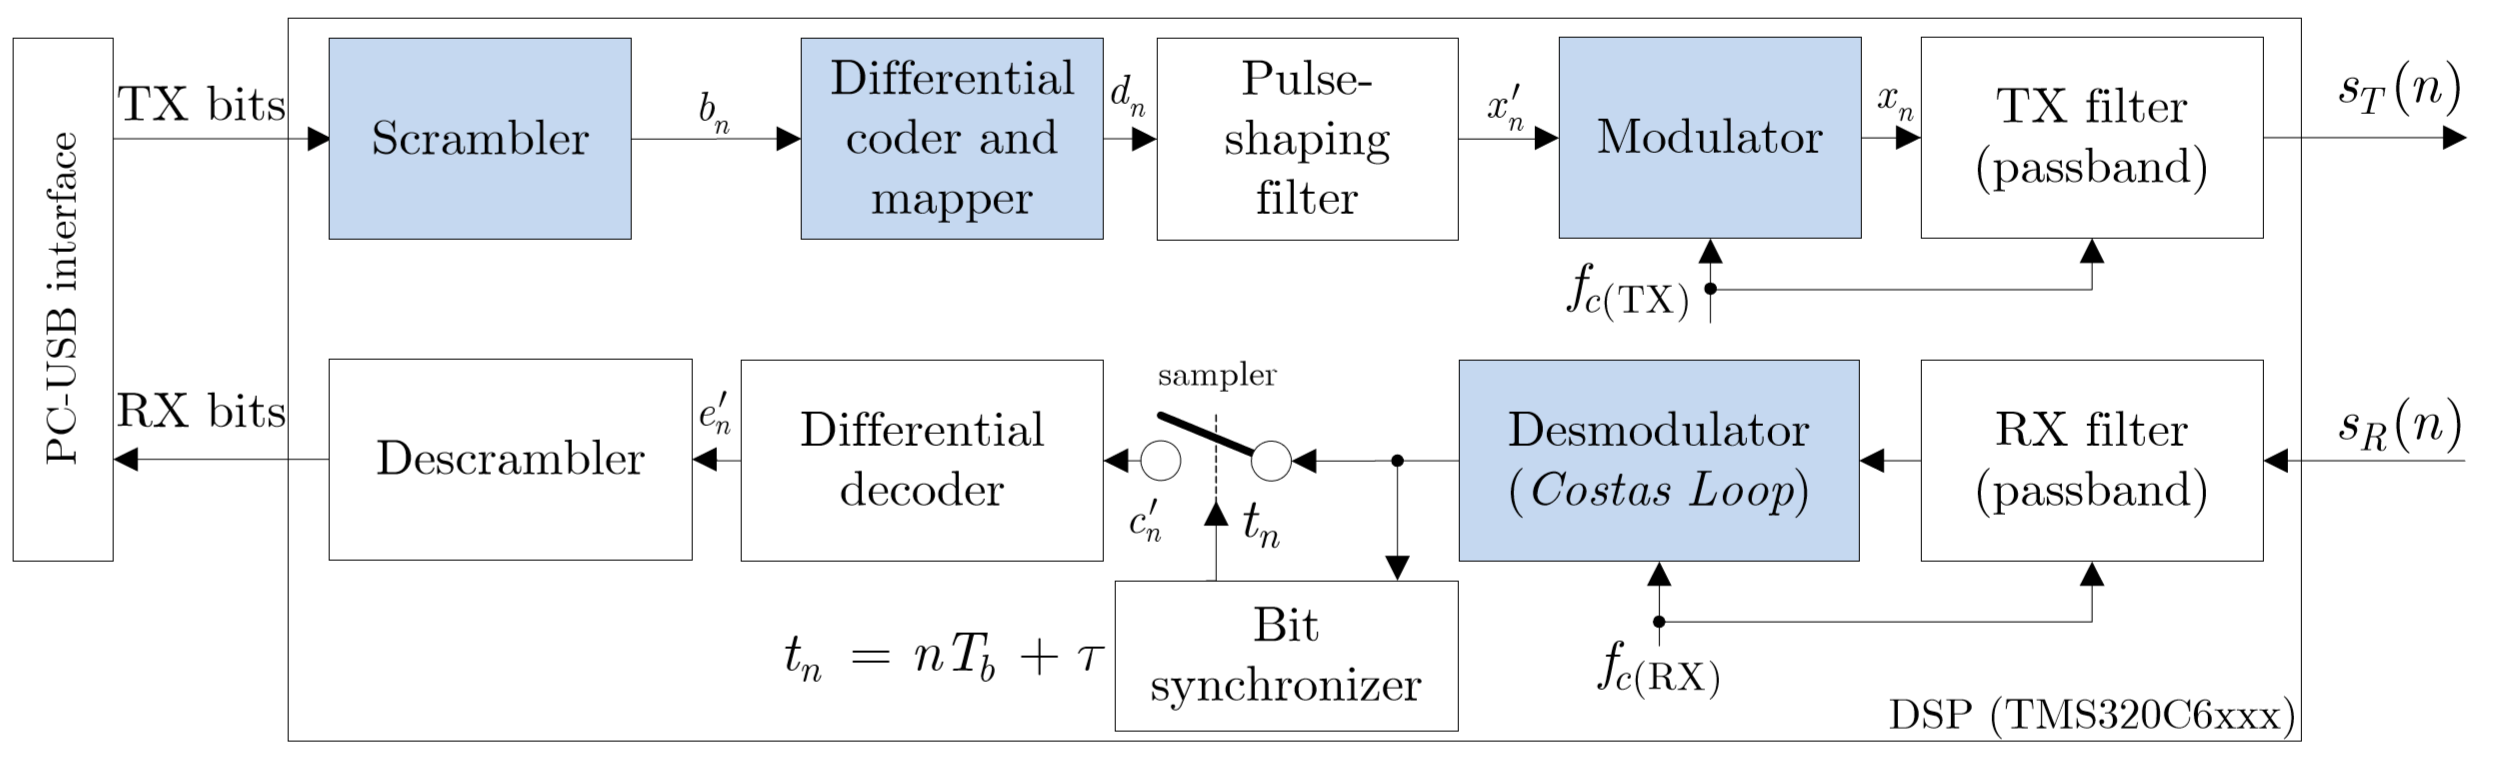
\includegraphics[keepaspectratio=true, scale=0.30]{teoricas/modem}
	\caption{\textit{Modem} DSP-BPSK.}
	\vspace{-0.8em}
\end{figure}

Na Figura 2 está representado o \textit{subset} do \textit{modem} BPSK a implementar.

\begin{figure}[H]
	\centering
	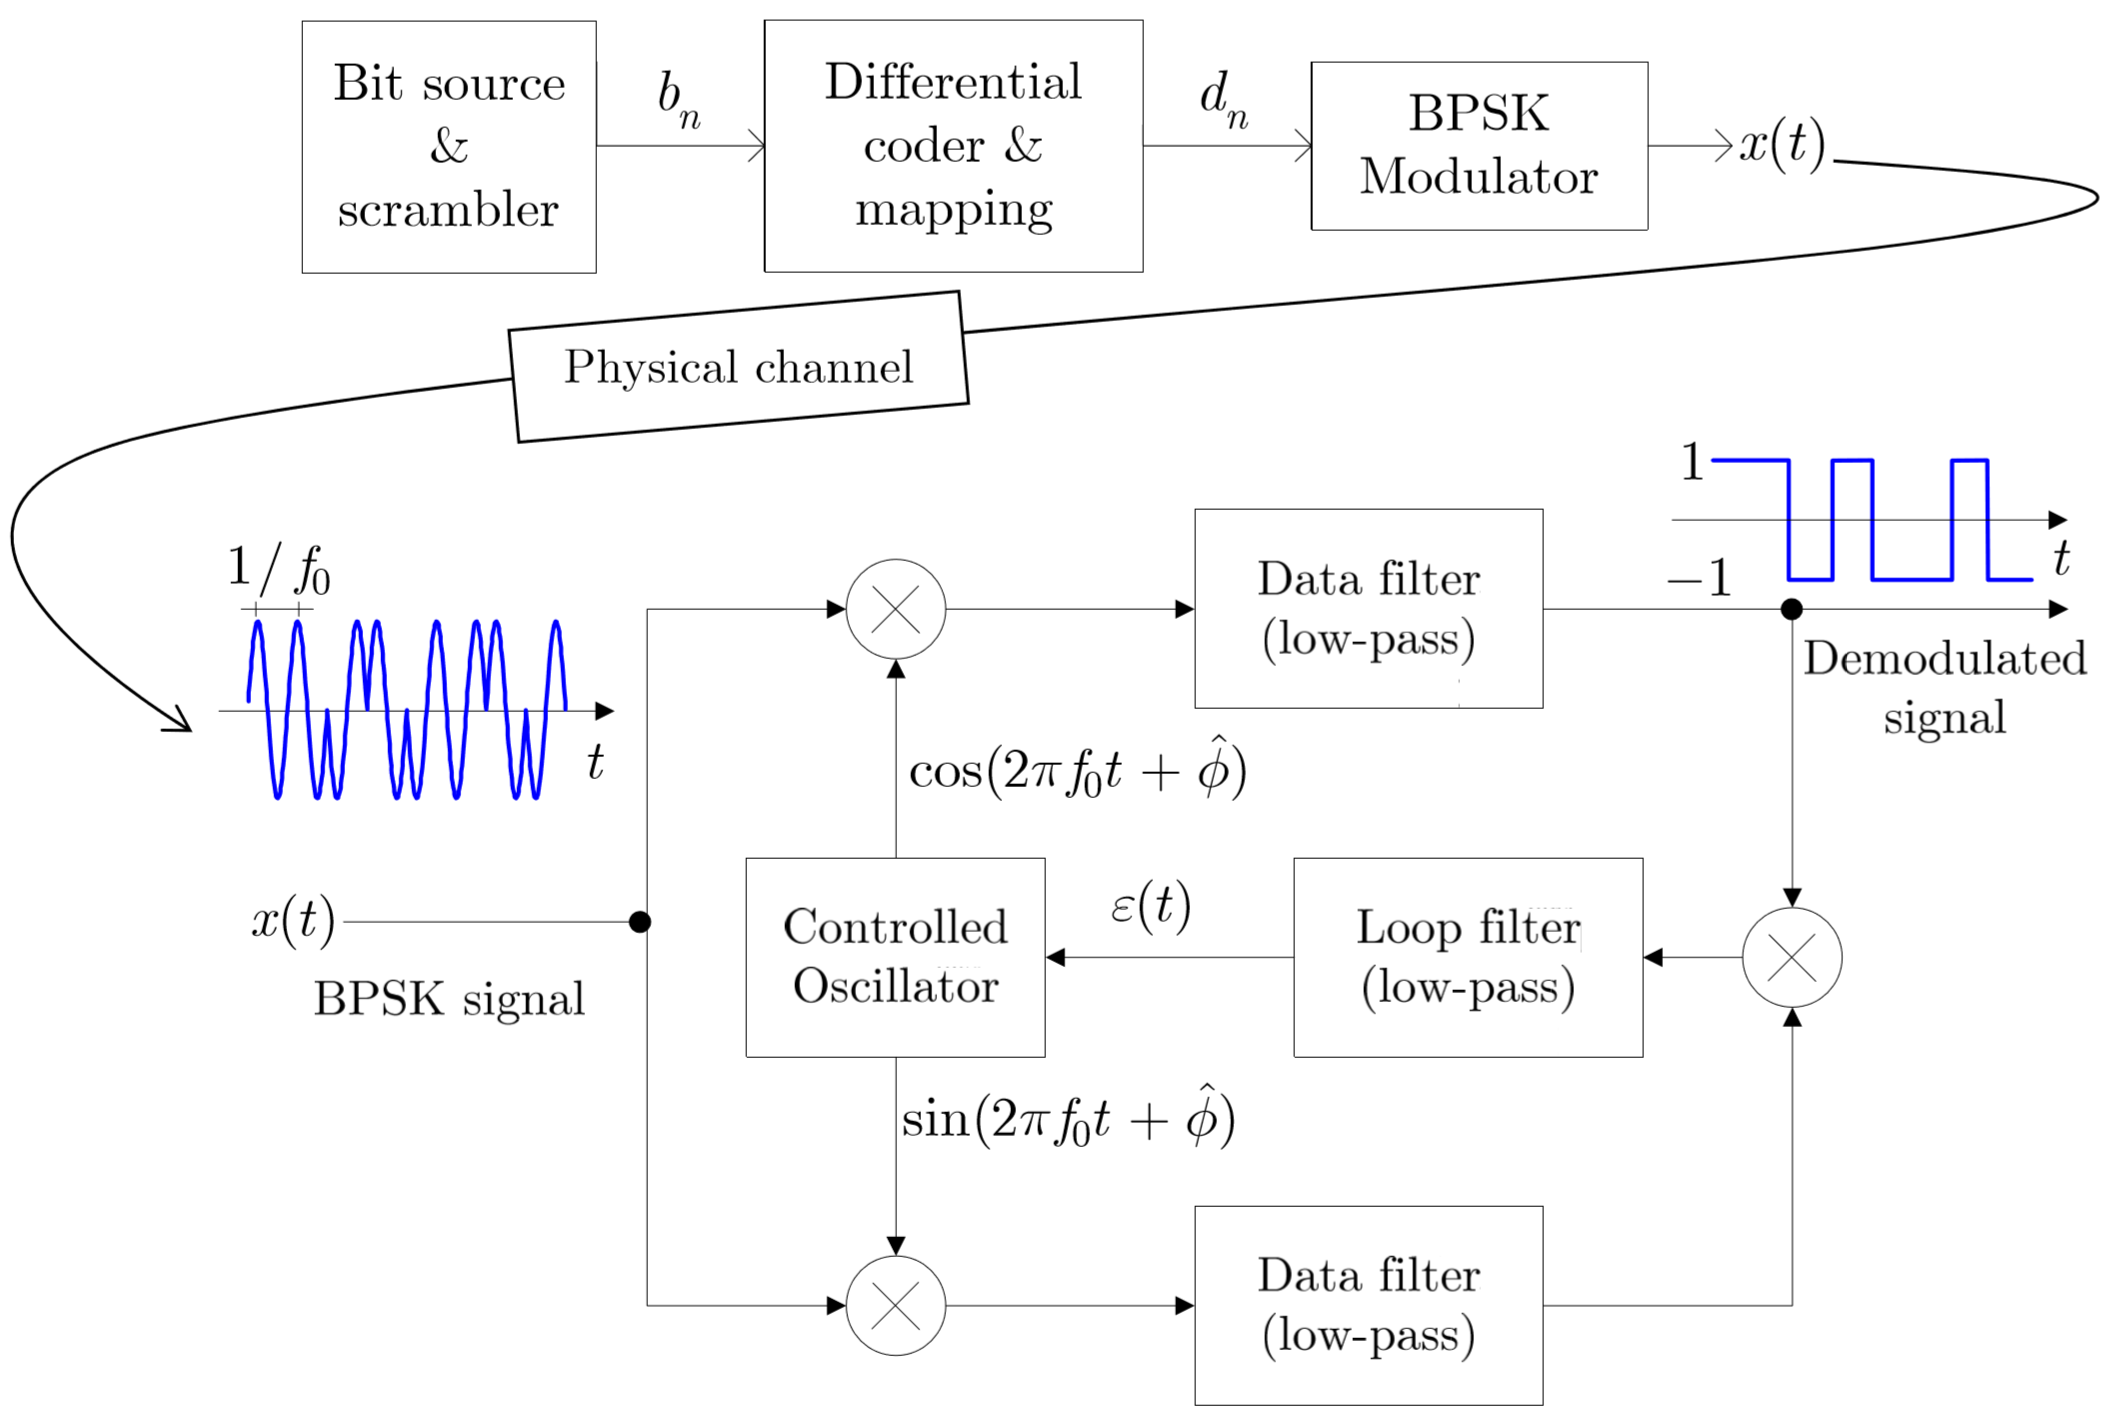
\includegraphics[keepaspectratio=true, scale=0.27]{teoricas/modem2}
	\caption{\textit{Subset} do \textit{modem} BPSK a implementar.}
	\vspace{-0.8em}
\end{figure}

\pagebreak

\section{Projecto de Demonstração}

Com o objectivo de fazer uma adaptação às ferramentas de trabalho realiza-se um projeto de demonstração que reproduz um seno através de uma \textit{look-up-table} (LUT) de 8 posições, como se pode ver no excerto de código seguinte.

\begin{lstlisting}[language=C]
	...
		//LUT do seno
		short sine_table[8] = {0,707,1000,707,0,-707,-1000,-707}; 
	...
\end{lstlisting}

Esta LUT é lida num \textit{loop} e os seus valores são multiplicados por um factor de ganho antes de serem exibidos no osciloscópio, ou seja, ocorre uma multiplicação de duas variáveis do tipo \texttt{short} com representação em $Q_{15}$. O formato do resultado da multiplicação de duas variáveis em $Q_{15}$ é $Q_{30}$ com replicação do \textit{bit} de sinal. Assim, é necessário efectuar um \textit{shift} para a esquerda para remover o \textit{bit} de sinal replicado, resultando num formato final de $Q_{31}$, para 32 bits. Para se poder armazenar numa variável de 16 \textit{bits}, no formato $Q_{15}$, é necessário efectuar um \textit{shift} de 16 posições para a direita, permitindo armazenar os 16 \textit{bits} mais significativos do resultado de 32 \textit{bits}. 

Em complemento para dois e numa notação do formato $Q_{15}$ pode-se representar valores no intervalo $-2^{0} \leq x \leq 2^{0} - 2^{-15}$, o que corresponde a valores decimais entre -32767 e 32767. Quando é atingido o valor máximo, 32767, entra em efeito a circularidade da representação em complemento para dois e, assim, para este caso, o valor máximo da amplitude do seno não atinge o valor $2^{15}$, ``dando a volta'' para -32767. 

Com um valor inicial para o ganho de 10, o valor máximo de amplitude que ocorre no seno gerado é de $1000 \times 10 = 10000$, valor que se encontra compreendido no intervalo referido anteriormente. Também para um factor de ganho de 32 o valor máximo da amplitude do seno pode ser representada no formato $Q_{15}$. Porém, quando o factor de ganho passa para 33 esse valor máximo passa para $1000 \times 33 = 33000$, valor que gera um \textit{overflow}, como explicado anteriormente.

Para um factor de ganho de 10 os valores do seno para 8 iterações do \textit{loop} que o gera são $\{0,7070,10000,7070,0,-7070,-10000,-7070\}$ e para um factor de ganho de 33 os valores são $\{0,23331,$ \linebreak $-233,23331,0,-23331,233,-23331\}$. O valor de 233 deriva do \textit{overflow} gerado e a amplitude da sinusoide fica com o valor $33000 - 32767 = 233$.

Analisando os valores anteriores verifica-se que a sinusoide com o factor de ganho de 33 tem uma frequência que é o triplo da frequência da sinusoide com o factor de ganho de 10, como se pode ver na figura da próxima página.

\begin{figure}[H]
	\centering
	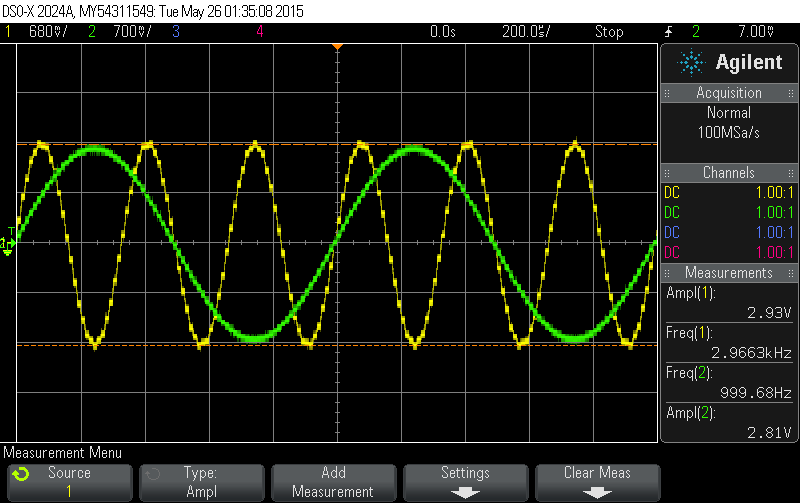
\includegraphics[keepaspectratio=true, scale=0.37]{exps/demonstracao}
	\caption{Sinusoide gerada para um factor de ganho de 10 (a verde) e para um factor de ganho de 33 (a amarelo).}
	\vspace{-0.8em}
\end{figure}

Verifica-se que a onda a verde tem uma frequência próxima de 1 kHz e a onda a amarelo tem uma frequência próxima de 3 kHz, ou seja, o triplo da frequência da sinusoide que tem um factor de ganho de 10.

\pagebreak

\section{Projecto $\#$1 - NCO}

Um oscilador numericamente controlado permite gerar uma frequência instantânea proporcional â amplitude do sinal de entrada. É um gerador digital de sinal que cria uma representação síncrona, discreta no tempo e discreta em amplitude de uma forma de onda.

As características do NCO são apresentadas na tabela seguinte.

\begin{table}[H]
	\centering
	\caption{Características do NCO.}
	\vspace{-1.5mm}
	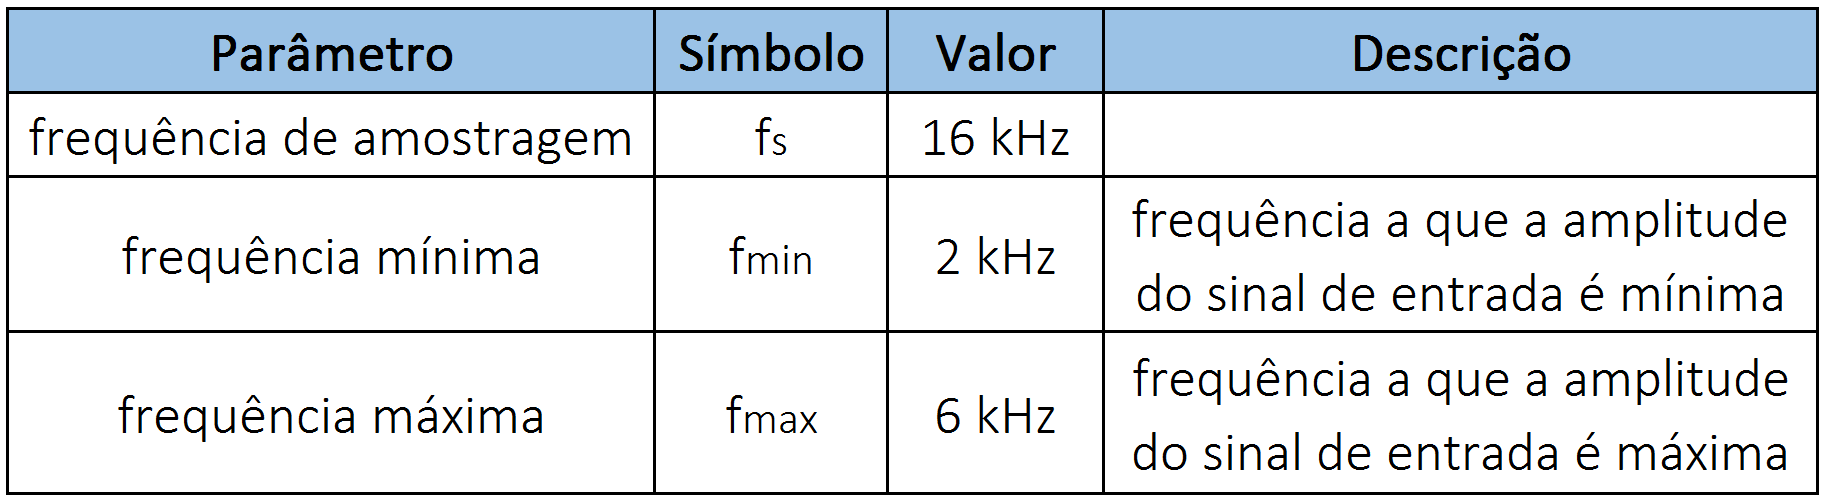
\includegraphics[keepaspectratio=true, scale=0.45]{tabelas/tabela1}
\end{table}

Pretende-se primeiramente desenvolver um oscilador de relaxação utilizando uma variável inteira com sinal de 16 \textit{bits} e a circularidade da representação em complemento para dois. Na figura abaixo encontra-se uma representação do sinal a obter.

\begin{figure}[H]
	\centering
	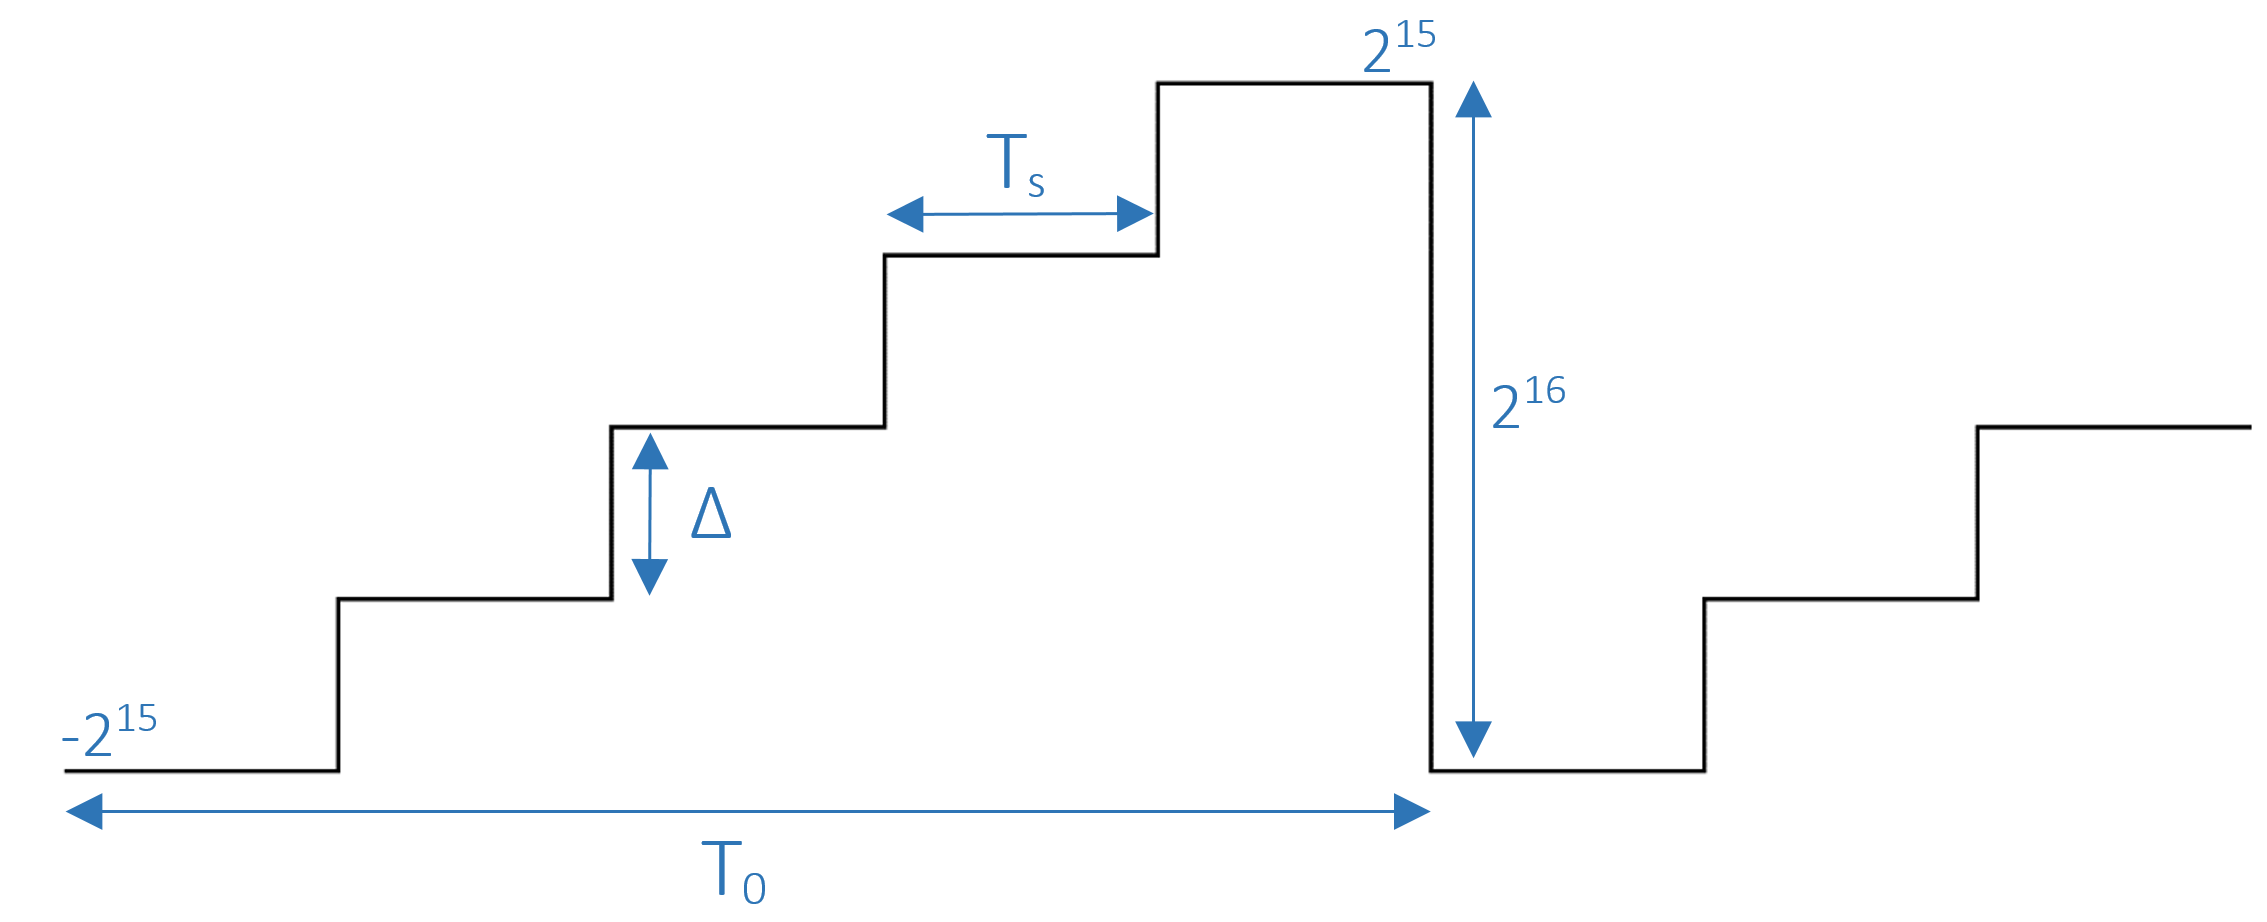
\includegraphics[keepaspectratio=true, scale=0.37]{teoricas/rampa}
	\caption{Esquema do oscilador de relaxação.}
	\vspace{-0.8em}
\end{figure}

Com recurso à Figura 1 pode-se deduzir que

\vspace{-3mm}
\begin{equation}
f_{0} = \frac{\Delta}{2^{16}} \times f_{s} \leftrightarrow \Delta = \frac{f_{0}}{f_{s}} \times 2^{16}.
\end{equation}

\vspace{1mm}
Existe uma variável de estado da rampa que a cada $T_{s}$, período de amostragem, é incrementada de $\Delta$, como se pode ver na Figura 1. A variável de estado da rampa é de 16 \textit{bits} com representação em $Q_{15}$ e, sabendo que o maior número positivo que se pode representar em $Q_{15}$ é $2^{15} - 1 = 32767$ e o menor número negativo que se pode representar é  $-(2^{15} - 1) = -32767$, a variável de estado começa com o valor -32767 e vai até um máximo de 32767. Quando é atingido o valor máximo, 32767, entra em efeito a circularidade da representação em complemento para dois e, assim, a variável de estado não atinge o valor de $2^{15}$, ``dando a volta'' para -32767. 

Relativamente à variável $\Delta$ esta encontra-se também representada em $Q_{15}$. O NCO tem como característica uma frequência $f_{0}$ que varia entre 2 kHz e 6 kHz. Estes valores são controlados a partir da amplitude do sinal de entrada. Quando esta for mínima, a frequência $f_{0}$ é de 2 kHz e quando for máxima, a frequência $f_{0}$ é de 6 kHz. Com estas especificações pode-se calcular três valores de $\Delta$ com recurso à equação (2.1), para a frequência mínima, a frequência média e a frequência máxima.

\begin{table}[H]
	\centering
	\caption{Valores de $\Delta$ para as três frequências especificadas.}
	\vspace{-1.5mm}
	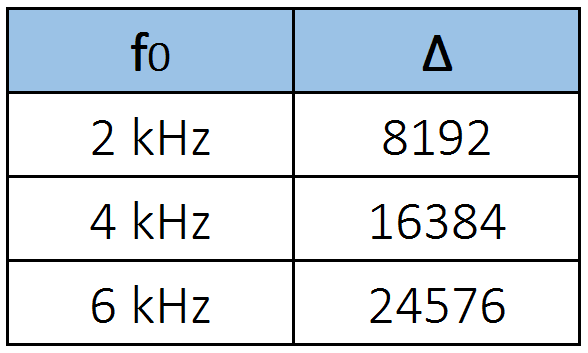
\includegraphics[keepaspectratio=true, scale=0.45]{tabelas/tabela2}
\end{table}

Em código, a variável de estado da rampa é \texttt{status} e a variável que representa os incrementos é \texttt{delta}. No código abaixo está a criação da rampa para um frequência de 4 kHz.

\begin{lstlisting}[language=C]
void main(){

	short delta = 16384;
	short status = -32767;

	while(1){
		...	
		//criacao da rampa	
		status = status + delta;
		...
	}
}
\end{lstlisting}

Nas figuras da próxima página pode-se ver o sinal obtido experimentalmente que representa a rampa para dois valores diferentes de frequência $f_{0}$.

\begin{figure}[H]
	\centering
	\subfloat[]{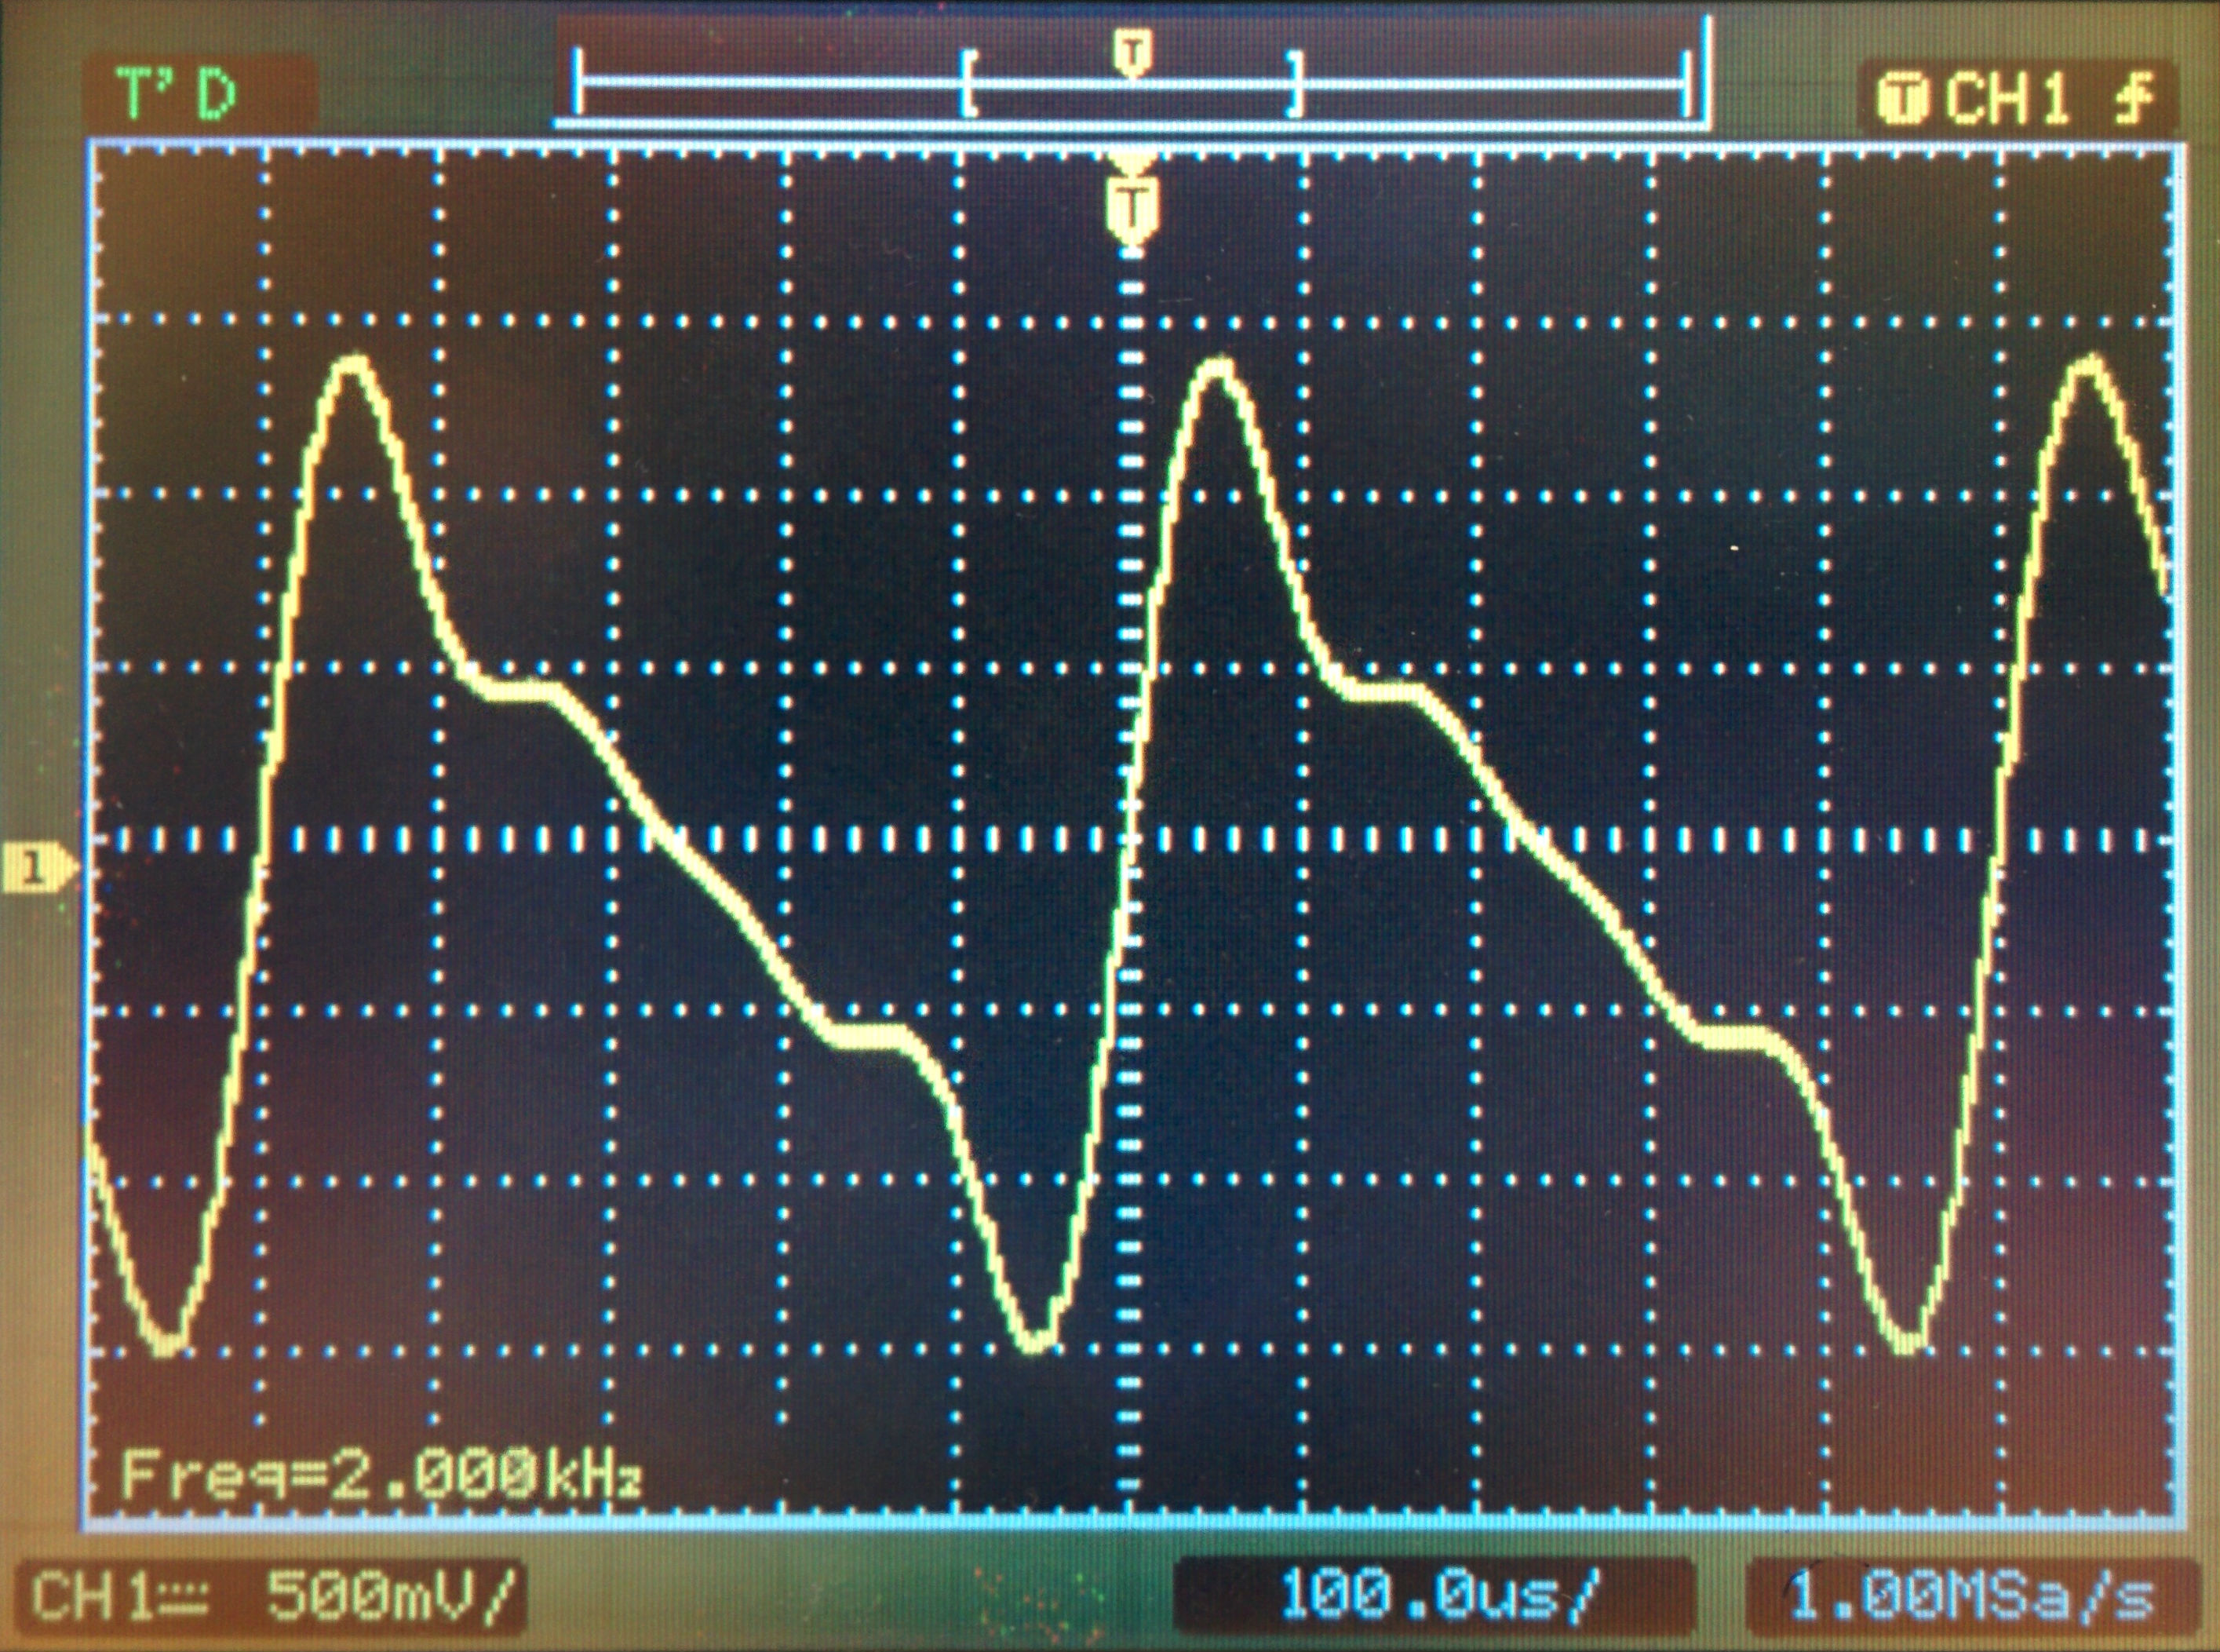
\includegraphics[keepaspectratio=true, scale=0.073]{exps/rampa2K}}
	\hspace{8mm}
	\subfloat[]{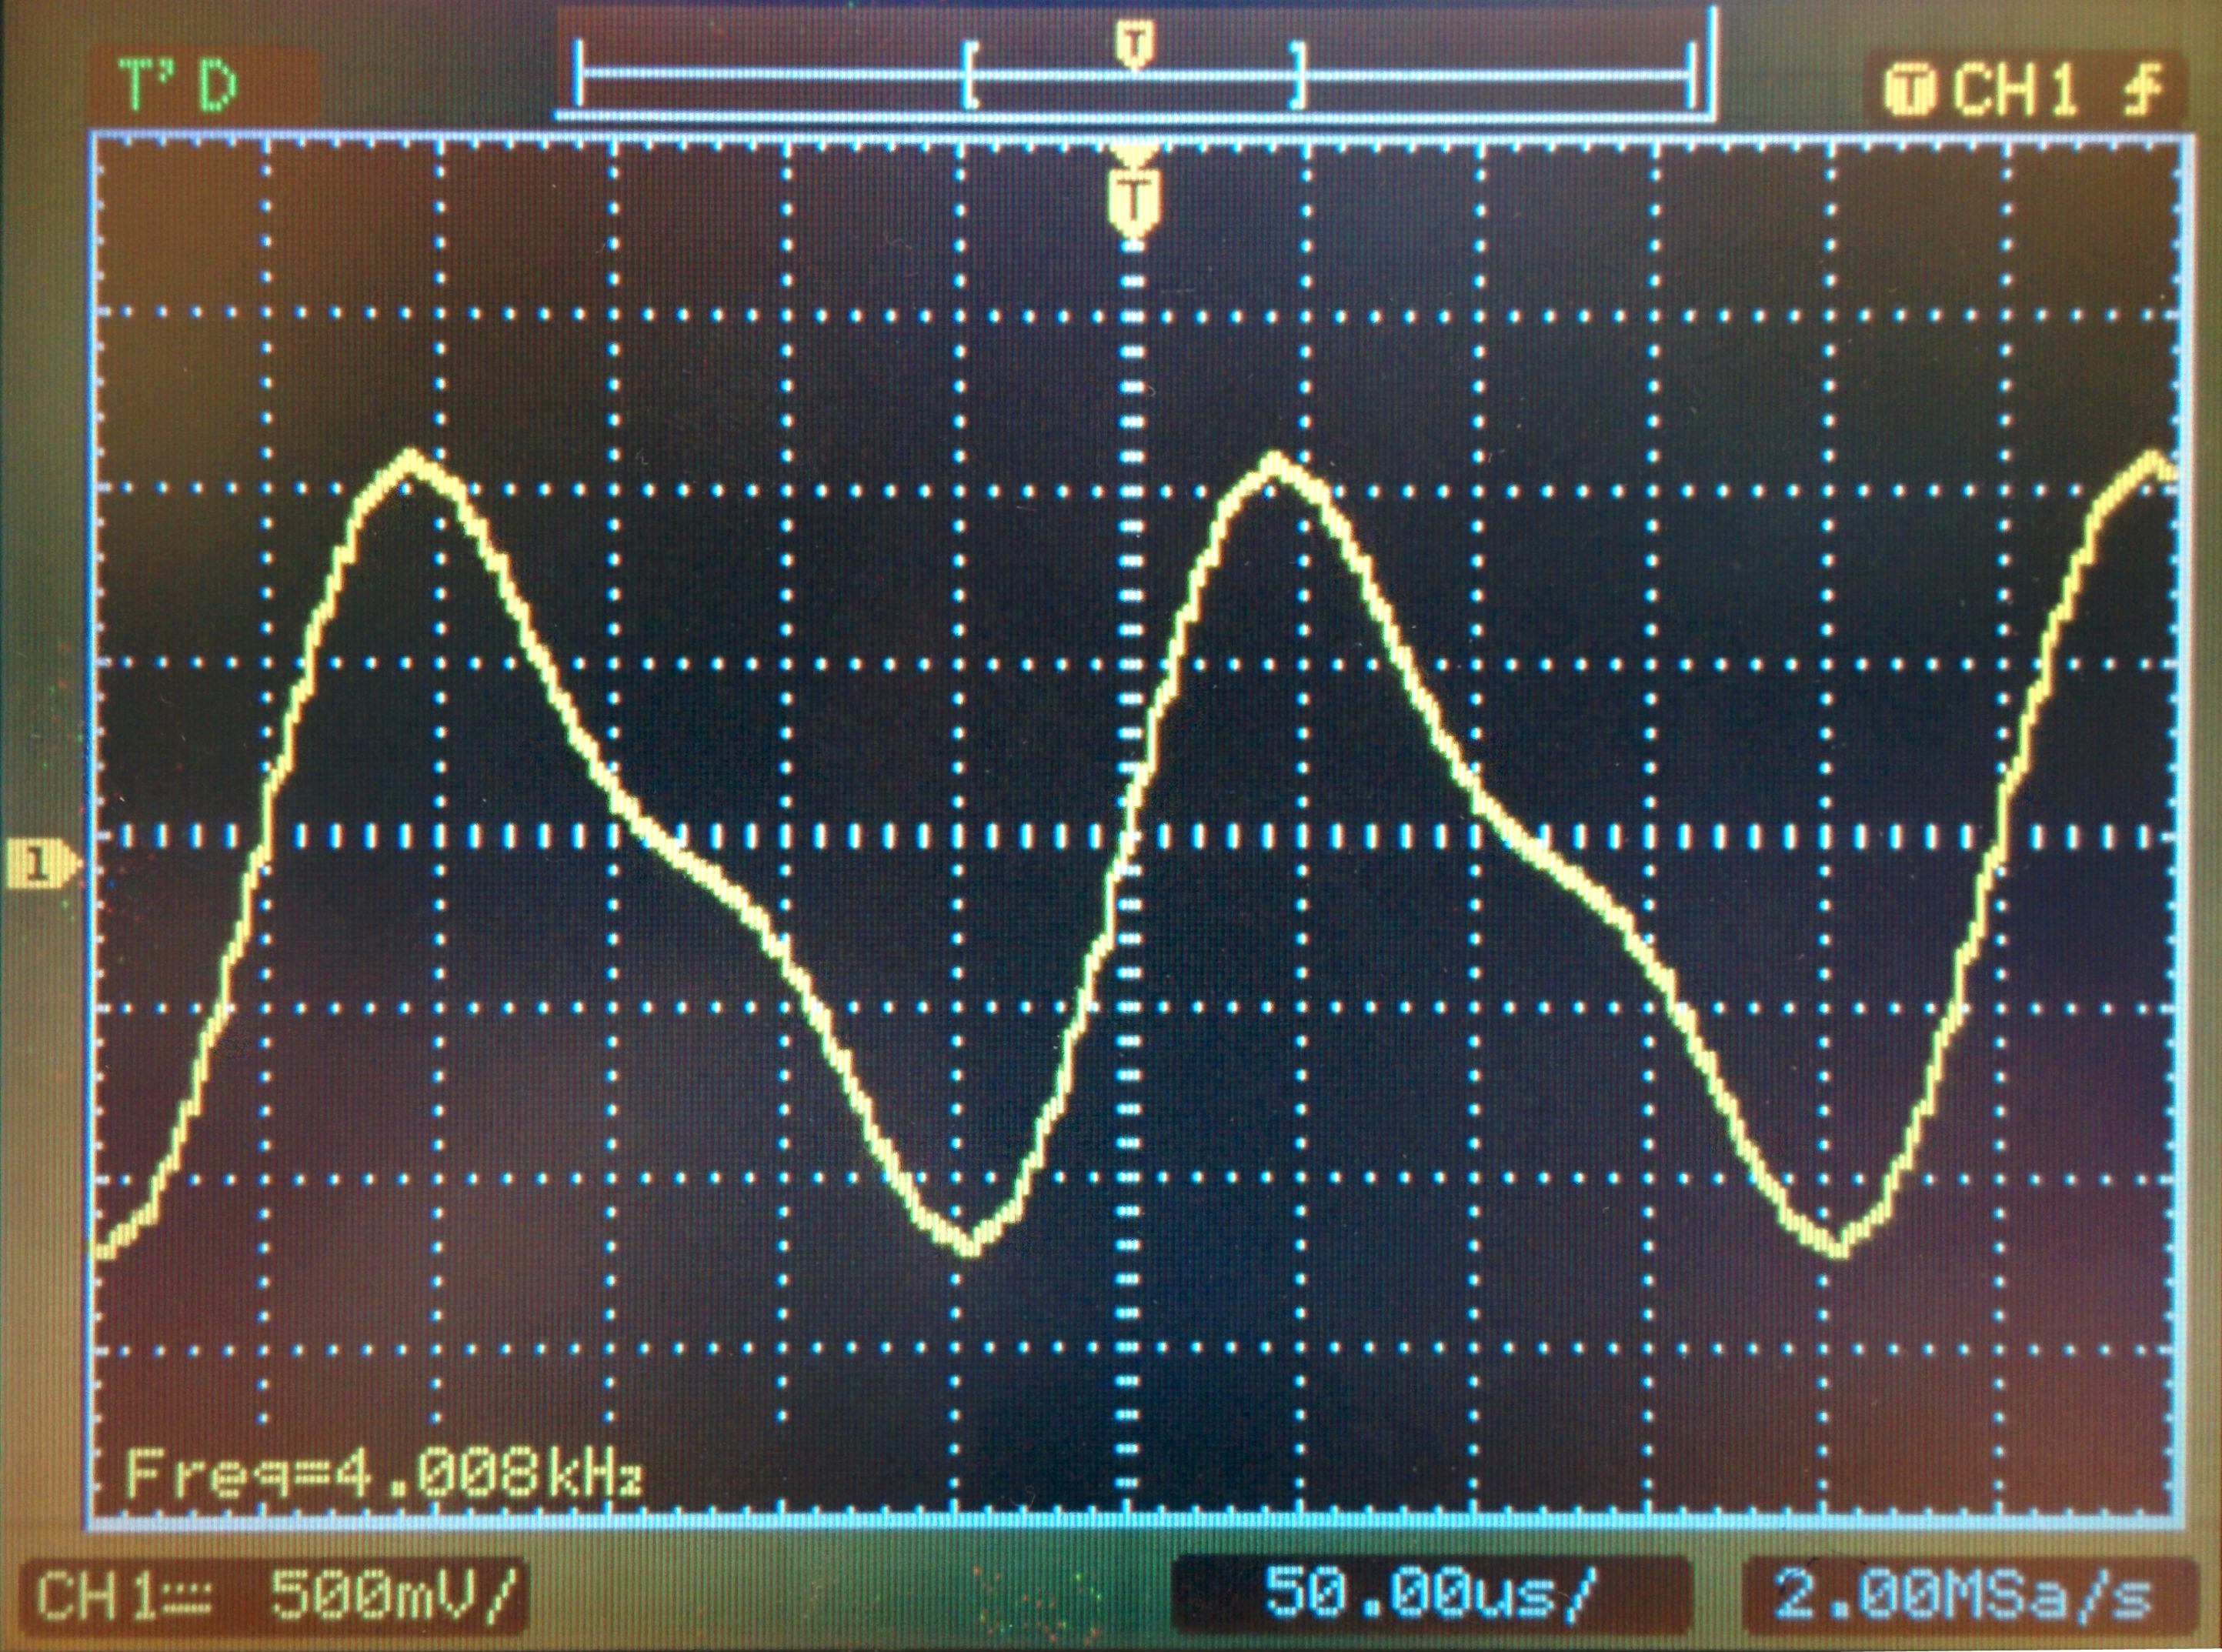
\includegraphics[keepaspectratio=true, scale=0.0719]{exps/rampa4K}}
	\linebreak
	\subfloat[]{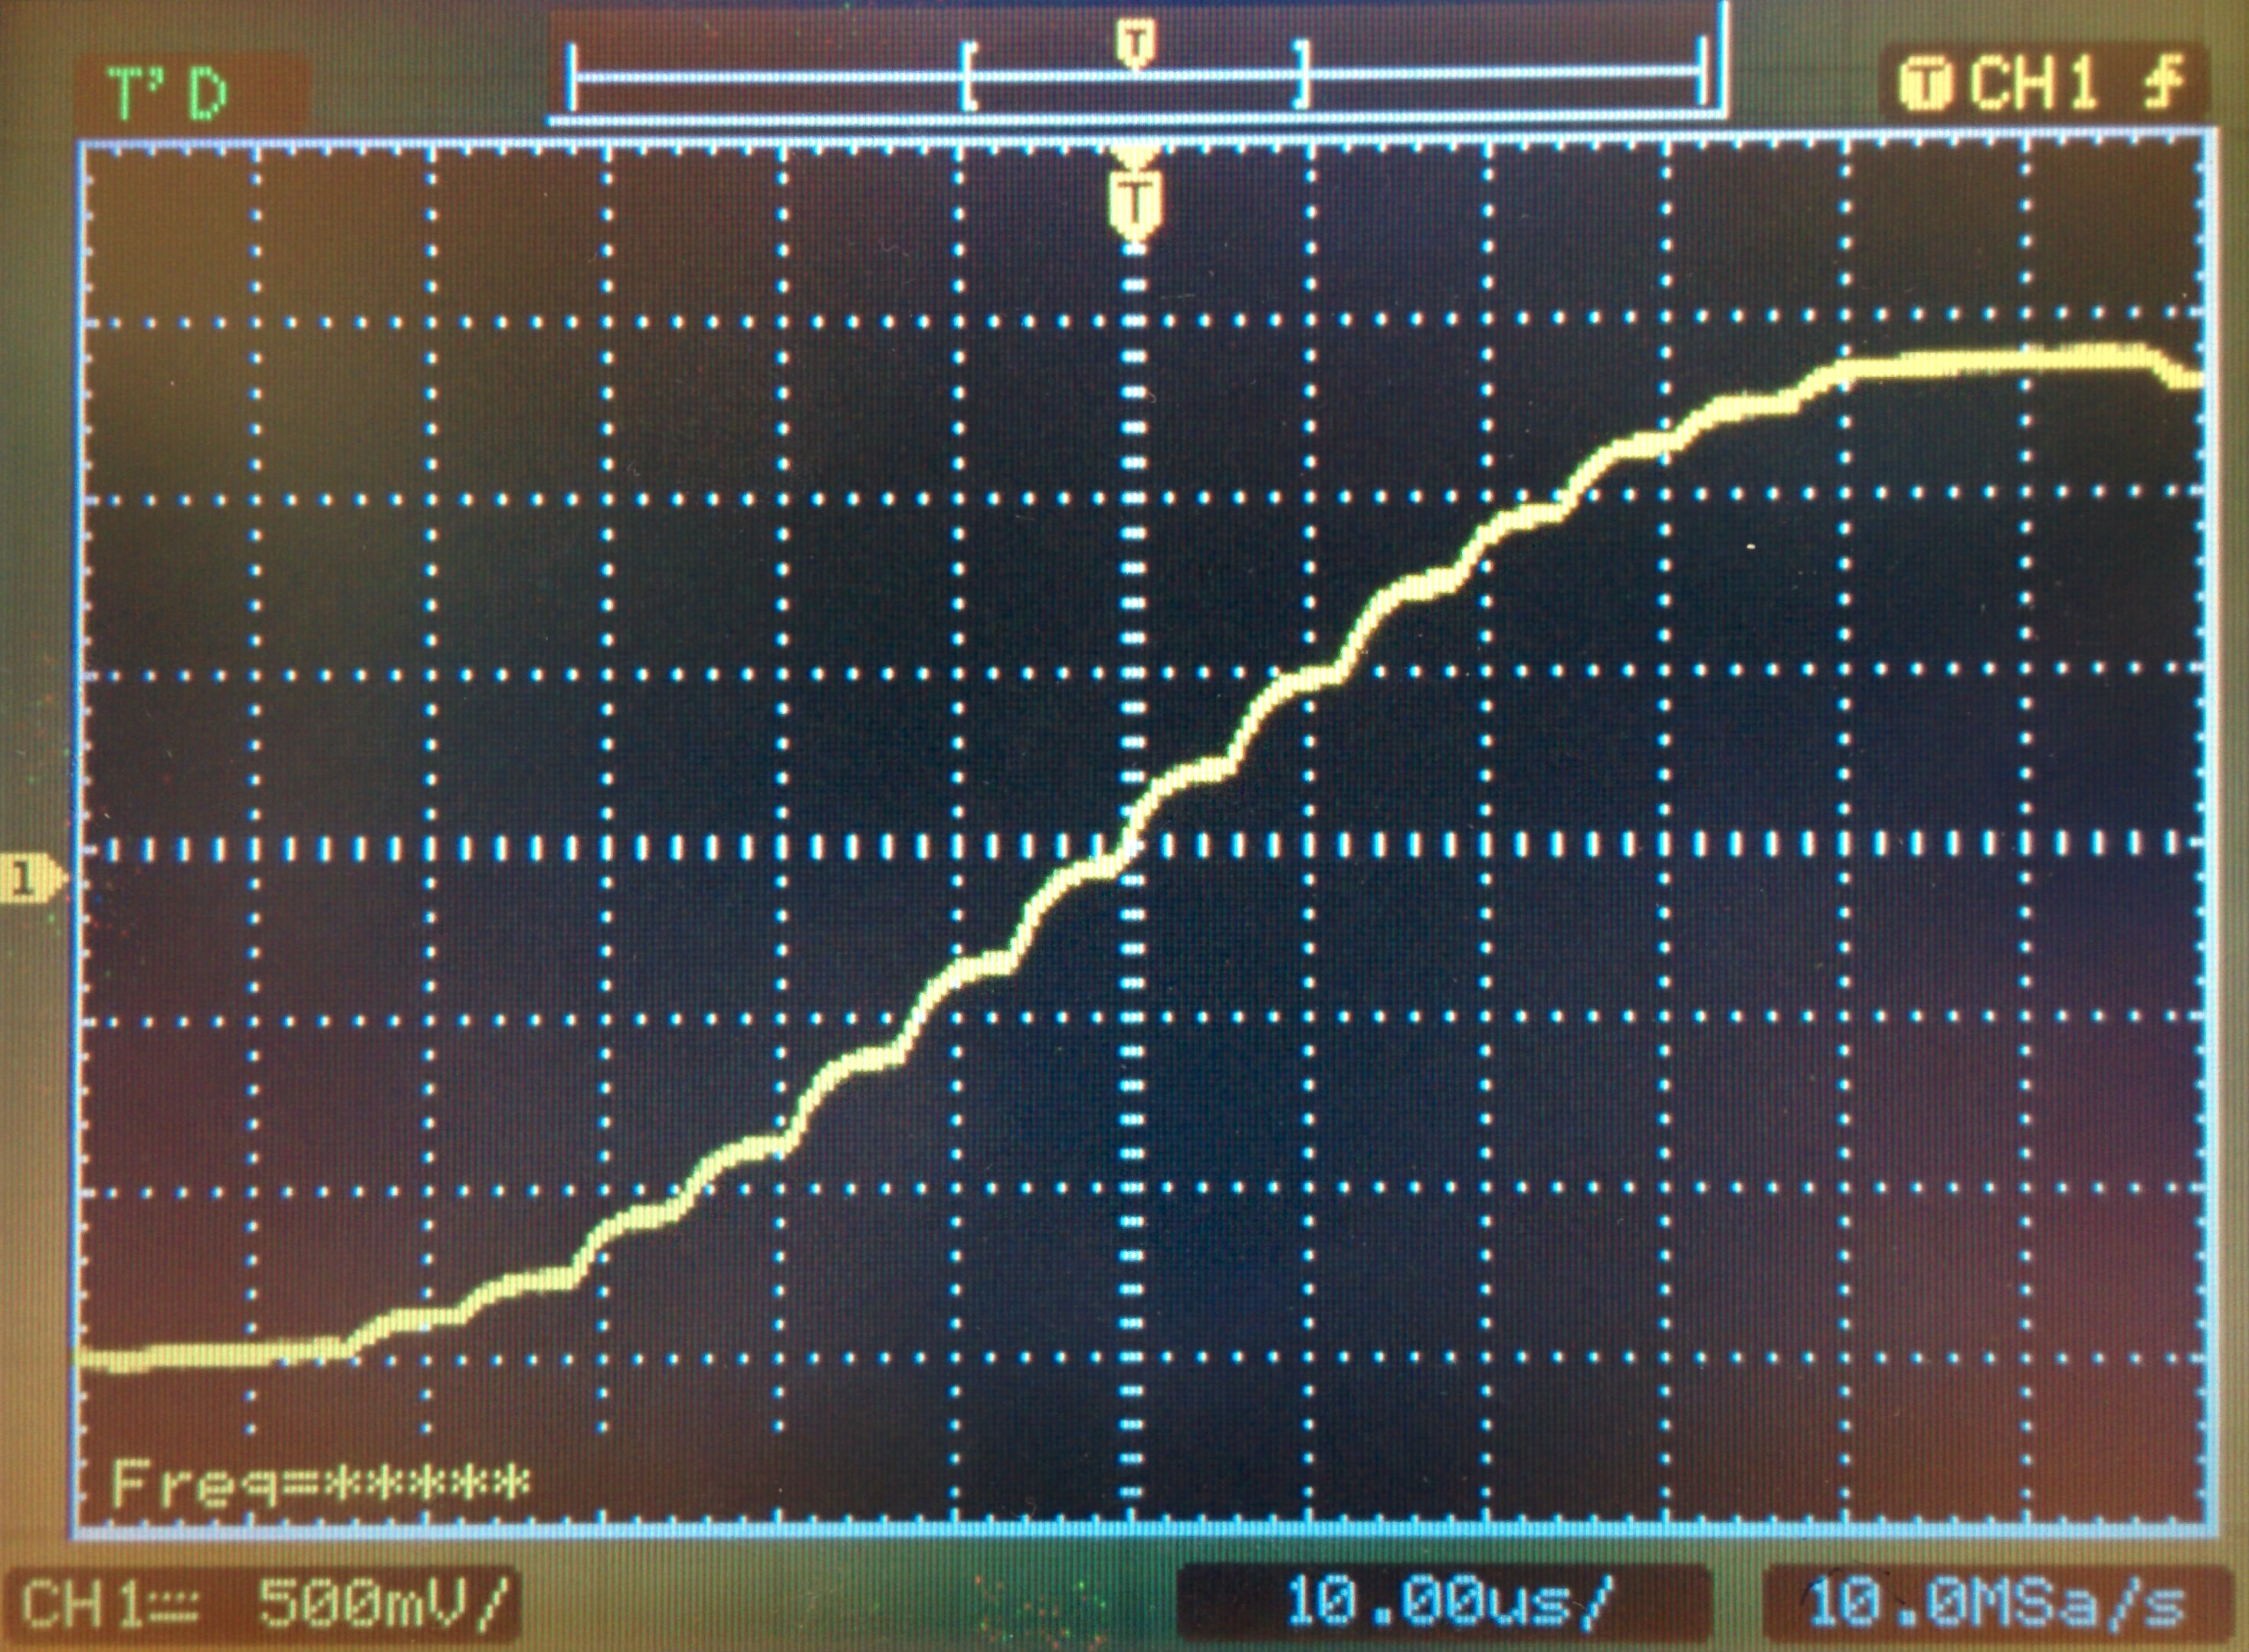
\includegraphics[keepaspectratio=true, scale=0.073]{exps/zoomrampa}}
	\vspace{-0.8em}
	\caption{Oscilador de relaxação para $f_{0}$ = 2 kHz (a), oscilador de relaxação para $f_{0}$ = 4 kHz (b) e pormenor da rampa criada (c).}
	\vspace{-0.8em}
\end{figure}

Como se pode ver na Figura 2(c), por comparação com o esperado teoricamente da Figura 1, o oscilador de relaxação implementado funciona de acordo com o previsto. De notar que o sinal que se observa está invertido relativamente ao teórico, o que já é esperado, quando se considera que antes de ser observado no osciloscópio passa por um inversor.

Com o oscilador implementado pretende-se agora criar uma LUT com 32 valores positivos de meio período da função seno. É necessário começar por determinar esses valores, para que, posteriormente, os mesmos sejam convertidos para o formato mais preciso de representação, $Q_{15}$, uma vez que se encontram no intervalo [-1, 1]. Assim, tendo em conta que meio período da função seno é $\pi$, podemos calcular os valores da seguinte maneira:

\vspace{-3mm}
\begin{equation}
a_{k} = \sin \left( \frac{\pi}{32}k \right), k = 0, 1, \ldots, 31.
\end{equation}

\vspace{1mm}
Os 32 valores determinados são então convertidos para o formato $Q_{15}$, recorrendo a:

\vspace{-3mm}
\begin{equation}
a_{k_{15}} = \text{round}\left(a_{k} \times 2^{15} \right),
\end{equation} 

\vspace{1mm}
sendo assim criada a LUT pretendida.

Apresenta-se de seguida o excerto de código onde é declarada a LUT com os valores de meio período da função seno, no vector \texttt{sine} que tem 33 posições, cada uma de 16 \textit{bits}. 

\begin{lstlisting}[language=C]
	...
		//LUT do seno
		short sine[33] = {0,3212,6393,9512,12540,15447,18205,20788,23170,25330,27246,28899,30274,31357,		32138,32610,32767,32610,32138,31357,30274,28899,27246,25330,23170,20788,18205,	15447,12540,9512,6393,3212,0}; 
	...
\end{lstlisting}

Como se pode constatar, a LUT é declarada com 33 valores, o que se deve ao facto de ser necessário garantir que, quando o valor de \texttt{i} for igual a \texttt{32}, seja possível aceder ao valor da função seno correspondente, o que não seria possível caso a LUT fosse apenas declarada com 32 valores.
 
É possível implementar uma solução diferente, em que é realizada a operação lógica \texttt{AND} de \texttt{i} e \texttt{i+1} para o valor de \texttt{y1} e \texttt{y2} (necessário para o caso  da interpolação), respectivamente, com a máscara \texttt{31}, sendo a variável i incrementada,  de acordo com as seguintes linhas de código:

\begin{lstlisting}[language=C]
	...
		i = i&31;
		y1 = sine[i];
		y2 = sine[(i+1)];
		i++;
	...
\end{lstlisting}

Esta solução faz com que não seja necessário mais memória para criar a LUT, embora seja realizado um maior número de operações.  

Para que se possa agora aceder aos valores da função seno, é utilizada a variável de estado do oscilador, \texttt{status}, como índice da LUT. Apenas 5 \textit{bits} da variável são utilizados para endereçar a LUT, sendo criada a variável \texttt{i}, tal como especificado na Figura 3, onde a variável de estado do oscilador é representada por \textit{x}.

\begin{figure}[H]
	\centering
	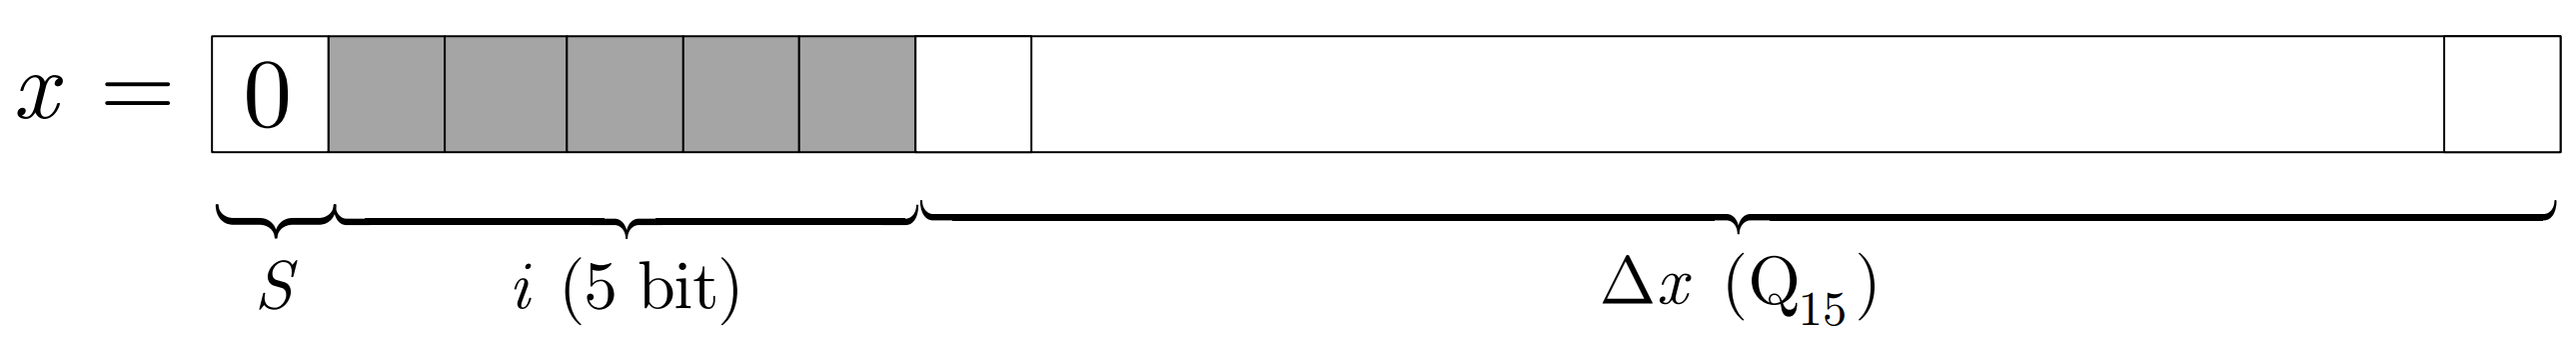
\includegraphics[keepaspectratio=true, scale=0.27]{teoricas/seno}
	\caption{Representação da variável do estado do oscilador.}
	\vspace{-0.8em}
	\label{fig:variavelestado}
\end{figure}

De modo a aceder aos 5 \textit{bits} pretendidos da variável de estado, é realizado um deslocamento de 10 \textit{bits} para a direita, sendo, de seguida, utilizada a função lógica \texttt{AND} com a máscara \texttt{31} (5 \textit{bits} menos significativos com o valor lógico \texttt{1}). É apresentado o excerto de código que realiza o procedimento especificado. 

\begin{lstlisting}[language=C]
	...
		//indexar a LUT e obter os valores do seno
		i = (status>>10)&31;
		y1 = sine[i]; 
	...
\end{lstlisting}

\change{david - aqui o prof tambem se queixou do and com 31}

Foram depois criadas duas variáveis com o objectivo de controlar a amplitude e frequência do sinal sinusoidal. A variável \texttt{delta} representa o controlo da frequência e a variável \texttt{amp} representa o controlo da amplitude. O código que permite implementar este controlo é apresentado de seguida.  

\begin{lstlisting}[language=C]
void main(){
	...
	//variavel de controlo de frequencia
	short delta = 0
	//variavel de controlo da amplitude: define um ganho de 1/2 
	short amp = 16384; 
	short yf = 0;
	...
	while(1){          
		if(intflag != FALSE){
		...	
		//obtencao do valor para a frequencia		
		delta = 16384 + (inbuf>>2); 
		 ...
		//controlo da amplitude e frequencia
		yf = (y1*delta<<1)>>16);
		y = (yf*amp<<1)>>16);
		
		if(status < 0)
			y = -y;
			
		AIC_buffer.channel[LEFT] = y;
		}
	}
}
\end{lstlisting}

Analisando a Tabela 2 verifica-se que o valor de \texttt{delta} oscila com uma amplitude de 8192 em torno de 16384, $\Delta_{0}$. Ou seja, $f_{0}$ tem uma frequência central em 4 kHz, oscilando com uma amplitude de 2 kHz. O incremento do oscilador é obtido de acordo com a seguinte equação, onde $x$ é a amplitude do sinal de entrada: 

\vspace{-3mm}
\begin{equation}
\Delta = \Delta_{0} + kx.
\end{equation}

\vspace{1mm}
Com esta conclusão, teve de se garantir que o valor da amplitude do sinal de entrada não ultrapassa 8192, mantendo a relação entre cada amostra. Optou-se por dividir o valor de cada amostra por 4, $k = 1/4$, pois a amplitude máxima é de 32767, o equivalente a um \textit{shift} de 2 \textit{bits} para a direita. 

Em baixo está o código referente ao cálculo para obter o valor de \texttt{delta}, sendo que todas as variáveis definidas neste excerto são de 16 \textit{bits}, \texttt{short}, em formato $Q_{15}$.

\begin{lstlisting}[language=C]
	...	
		//obtencao do valor para a frequencia		
		delta = 16384 + (inbuf>>2); 
	...
\end{lstlisting}

Tendo o valor de \texttt{delta}, é simples obter a amplitude de cada amostra do sinal de saída, somando  \texttt{delta} com \texttt{y1}, valor obtido da LUT especificada anteriormente. Em baixo está representado um excerto do código que demonstra a obtenção da amplitude do sinal de saída. Todas as variáveis são de 16 \textit{bits}, tendo \texttt{y1} e \texttt{delta} o formato de $Q_{15}$, como também \texttt{yf}. Isto deve-se ao facto de o formato do resultado da multiplicação com duas variáveis em $Q_{15}$ ser $Q_{30}$ com replicação do \textit{bit} de sinal. Assim, é necessário efectuar um \textit{shift} para a esquerda para remover o \textit{bit} de sinal replicado, resultando num formato final de $Q_{31}$, para 32 bits. Para se poder armazenar numa variável de 16 \textit{bits}, no formato $Q_{15}$, é necessário efectuar um \textit{shift} de 16 posições para a direita, permitindo armazenar os 16 \textit{bits} mais significativos do resultado de 32 \textit{bits}.

\change{teddy - neste paragrafo de cima, na 1a frase o prof colocou 2 ?}

O código apresentado de seguida demonstra a explicação referida.

\begin{lstlisting}[language=C]
	...
		//controlo de frequencia
		yf = y1 + delta;
	...
\end{lstlisting}


Para o controlo da amplitude do sinal de saída, multiplica-se o resultado final obtido anteriormente por uma constante de 16 \textit{bits} em formato $Q_{15}$. Está representado um excerto de código que demonstra a alteração da amplitude do sinal de saída. Neste caso todas as variáveis são também de 16 \textit{bits}, tendo \texttt{yf} e \texttt{amp} o formato de $Q_{15}$, como também \texttt{y}. Para armazenar a variável \texttt{y} em $Q_{15}$ recorre-se à mesma lógica explicada anteriormente de fazer 15 \textit{shifts} para a direita ao resultado da multiplicação.

O código apresentado de seguida demonstra a explicação referida.

\begin{lstlisting}[language=C]
	...
		//controlo da amplitude
		y = (y_f*amp<<1)>>16);
	...
\end{lstlisting}

Sabendo que os valores da LUT permitem aceder às arcadas positivas do seno, quando a variável de estado da rampa é negativa, \texttt{status} $<$ 0, o sinal de saída tem que ser negado. Em seguida está representado o código referente à explicação anterior:

\begin{lstlisting}[language=C]
	...
		if(status < 0){
			y = -y;
		}
	...
\end{lstlisting}

O sinal de saída pode ser observado no canal esquerdo da DSP.

\begin{lstlisting}[language=C]
	...
		AIC_buffer.channel[LEFT] = y;
	...
\end{lstlisting}

Com o oscilador controlado já implementado procede-se à fase de testes. A verificação de funcionamento pode ser vista na Figura 4, onde se utilizou um sinal de entrada, a verde, definido como uma onda quadrada com uma frequência de 200 Hz e uma amplitude próxima de 1 V, no intuito de poder verificar o controlo da frequência do sinal de saída, a amarelo, a partir da amplitude do sinal de entrada. 

Quando a amplitude do sinal de entrada é máxima pode-se visualizar um aumento da frequência do sinal de saída, ou seja, para um mesmo intervalo de tempo há um maior número de ciclos. Quando a amplitude do sinal de entrada é mínima, a frequência do sinal de saída diminui, ou seja, há um menor número de ciclos para o mesmo intervalo de tempo. Com estes resultados, pode-se concluir que o método de controlo utilizado funciona de modo adequado.

\change{na parte final do paragrafo o prof diz que temos de ter cuidado com esta conclusao pq ha um atraso de processamento}

\begin{figure}[H]
	\centering
	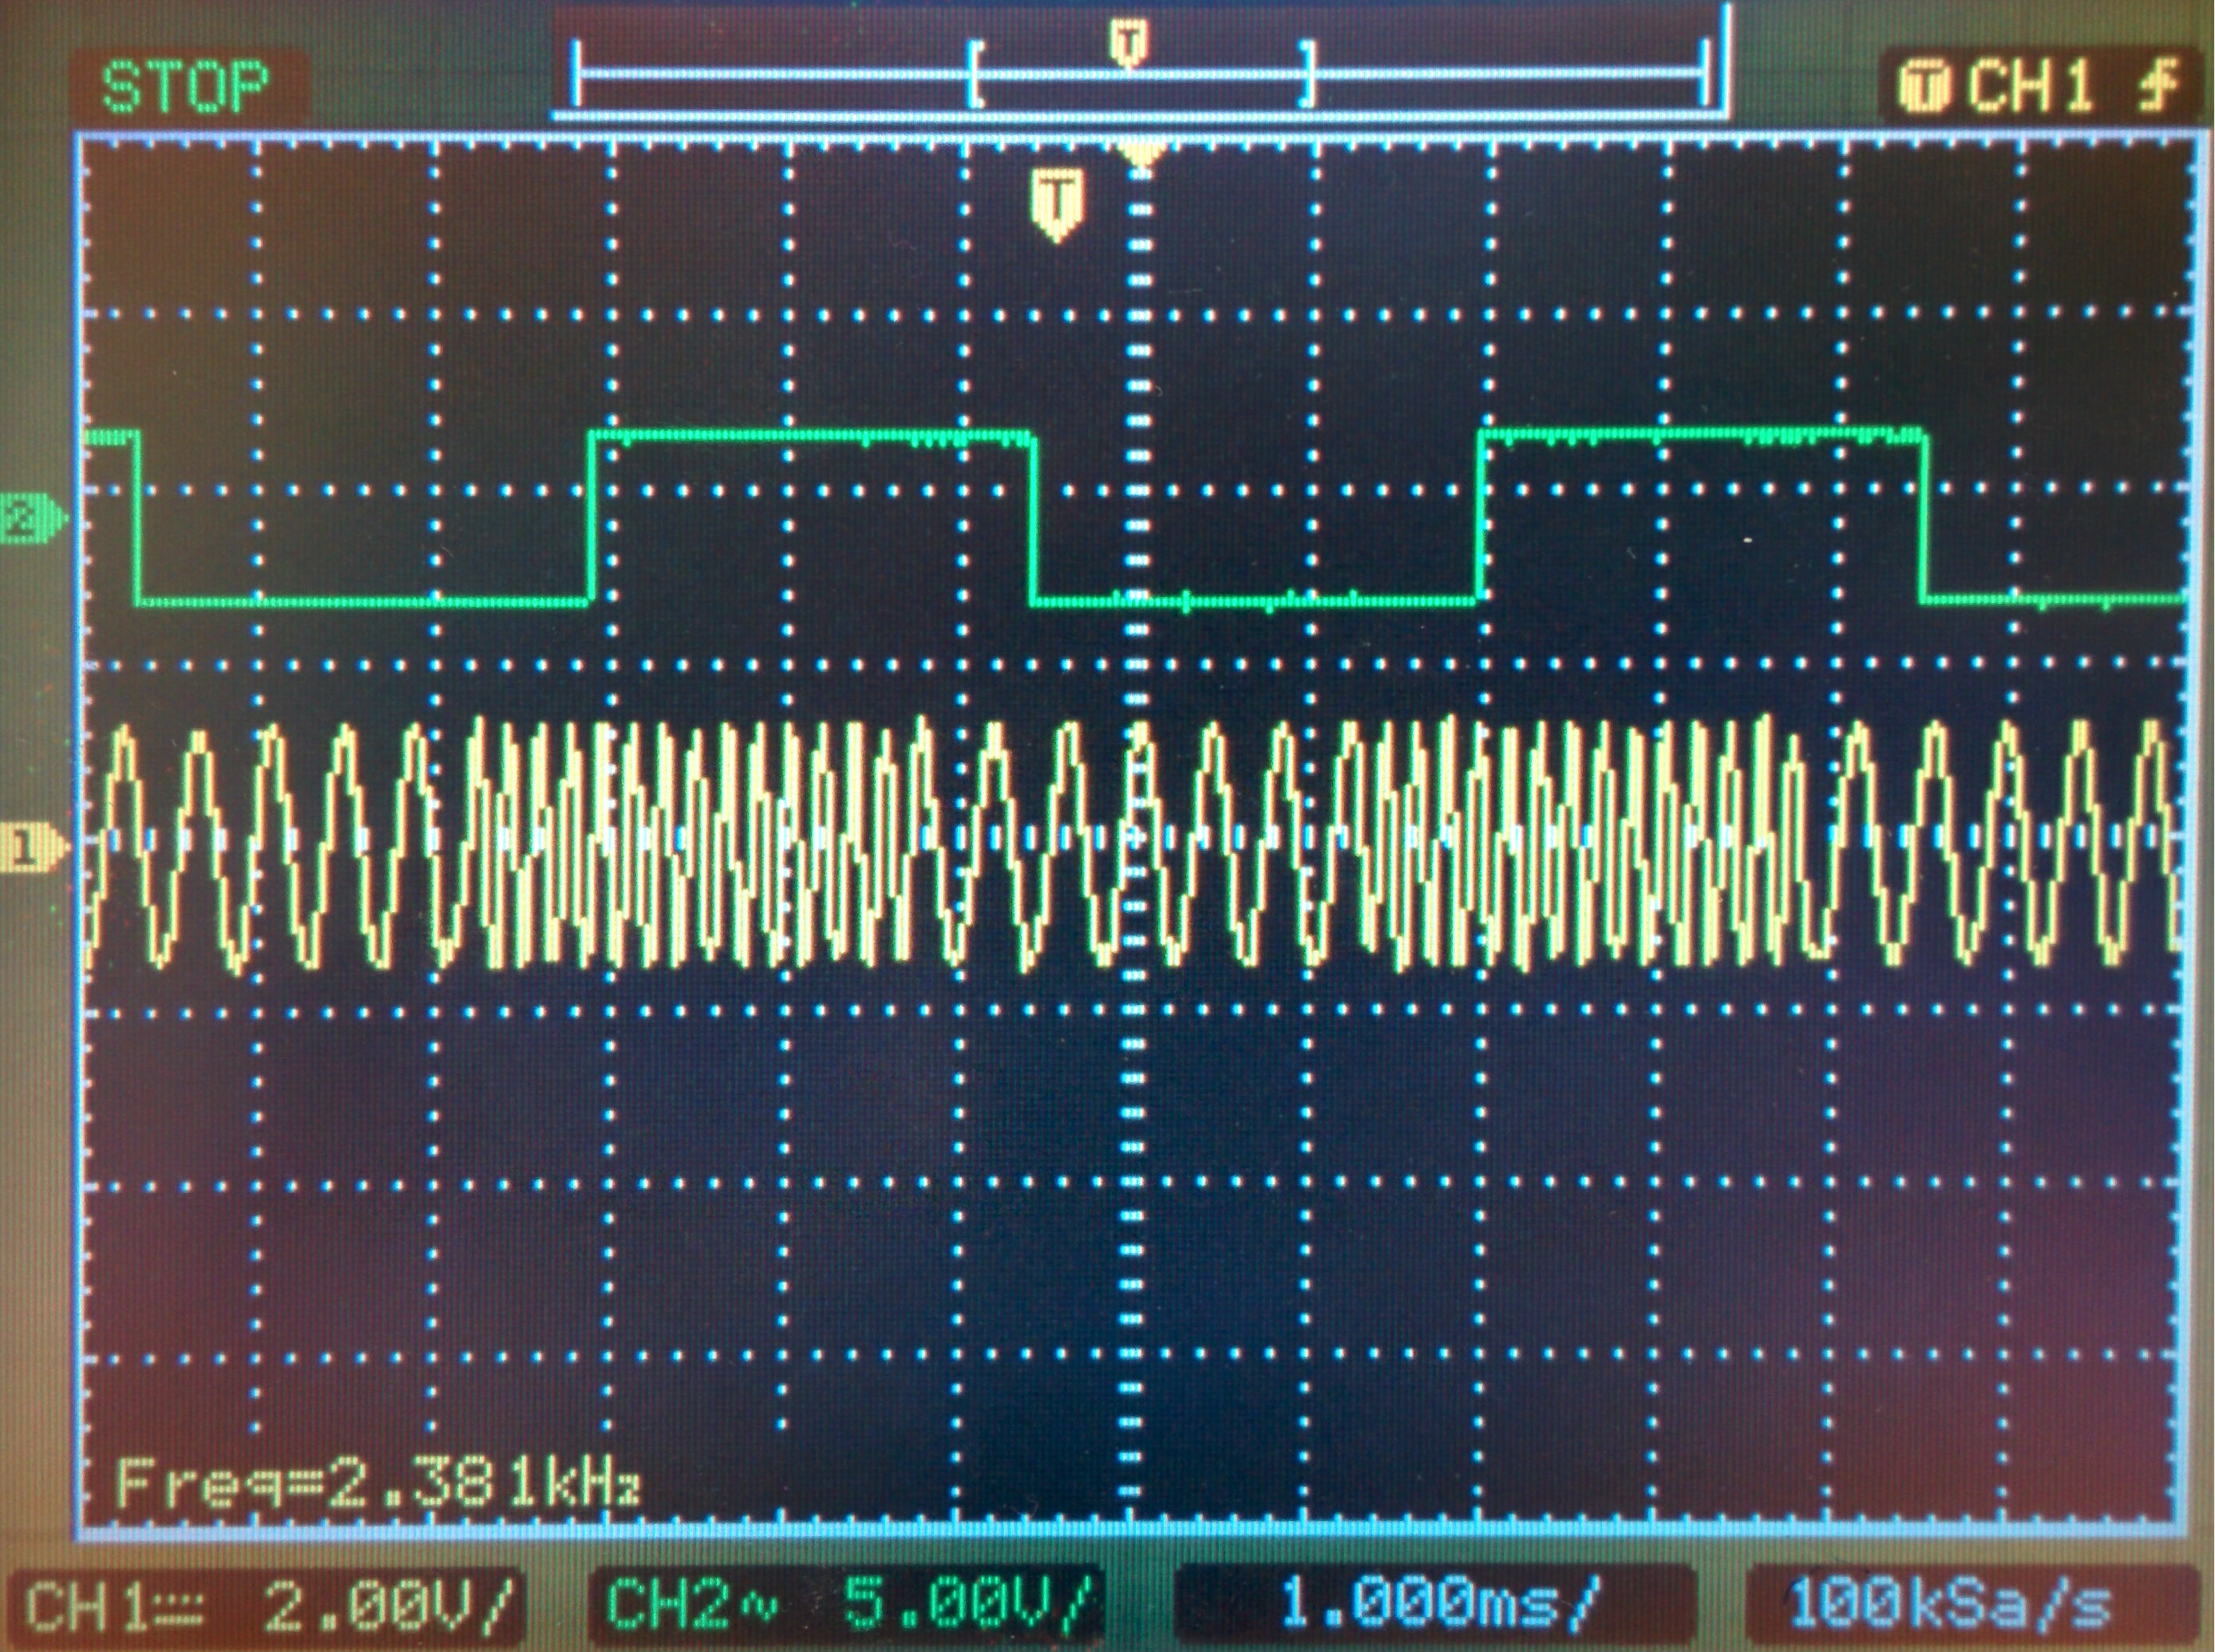
\includegraphics[keepaspectratio=true, scale=0.10]{exps/200Hz_2_6}
	\caption{Saída modulada na frequência do oscilador controlado (a amarelo) com \textit{input} de uma onda quadrada de 200 Hz (a verde).}
	\vspace{-0.8em}
\end{figure}

Pretende-se agora melhorar a qualidade do oscilador sinusoidal utilizando interpolação linear. Esta interpolação é feita lendo dois valores consecutivos, $y_{1}$ e $y_{2}$, da LUT do seno e depois obtém-se o valor sinusoidal interpolado com recurso à seguinte equação

\vspace{-3mm}
\begin{equation}
	y = y_{1} + (y_{2} - y_{1})\Delta x.
	\label{eq:interpol}
\end{equation}

\vspace{1mm}
Na Figura \ref{fig:variavelestado}, onde se encontra representada a variável de estado da rampa, pode-se ver que os 10 \textit{bits} menos significativos desta correspondem à variável $\Delta x$ da equação (\ref{eq:interpol}), que está representada no formato $Q_{15}$.

Para se obter o valor de $\Delta x$ é utilizada a função lógica \texttt{AND} com a máscara \texttt{1023} (10 \textit{bits} menos significativos com o valor lógico \texttt{1}), sendo de seguida necessário efectuar um \textit{shift} de 5 posições para a esquerda para que a variável seja representada em $Q_{15}$.

Com acesso a esse parâmetro, falta ler dois valores consecutivos da função seno, o que pode ser feito endereçando a LUT com recurso à variável \texttt{i} que foi anteriormente definida.

O excerto de código seguinte demonstra a obtenção do valor de $\Delta x$, armazenado na variável \texttt{delta\_x} e dois valores consecutivos da função seno, \texttt{y1} e \texttt{y2}.

\begin{lstlisting}[language=C]
	...
		//obtencao do valor de delta_x
		delta_x = (status&1023)<<5;
		i = (status >> 10) & 31;
		y1 = sine[i];
		y2 = sine[i+1];
	...
\end{lstlisting}

Pode-se agora computar $y$ de acordo com a equação (\ref{eq:interpol}). Quando se faz a subtracção entre $y_2$ ($Q_{15}$) e $y_1$ ($Q_{15}$), o resultado ficaria no formato $Q_{14}$. No entanto, dado que se subtraiem dois valores positivos em $Q_{15}$, tem-se a garantia de que o resultado é sempre correctamente armazenado em $Q_{15}$, o que é preferível face à opção de $Q_{14}$, pois garante mais resolução. 

O resultado desta subtracção é então multiplicado com $\Delta x$, que toma sempre valores entre 0 e 1, ou seja, está-se a multiplicar dois valores no formato $Q_{15}$, que origina um valor no formato $Q_{30}$ com replicação do \textit{bit} de sinal. Assim, é necessário efectuar um \textit{shift} para a esquerda para remover o \textit{bit} de sinal replicado, resultando num formato final de $Q_{31}$, para 32 bits. Para se poder armazenar numa variável de 16 \textit{bits}, no formato $Q_{15}$, é necessário efectuar um \textit{shift} de 16 posições para a direita, permitindo armazenar os 16 \textit{bits} mais significativos do resultado de 32 \textit{bits}.

O valor da subtracção que é seguida de uma multiplicação é agora somado ao valor de $y_1$, ou seja, está-se a somar dois números no formato $Q_{15}$, o que dá um resultado que seria no formato $Q_{14}$. No entanto, quando se analisa o pior caso em que $y_1$ = 32610, $y_2$ = 32767 e $\Delta x$ = 32767, o resultado da subtracção de $y_2$ com $y_1$ multiplicado por $\Delta x$ é igual a 5144419 em $Q_{31}$ ou 78 em $Q_{15}$, dividindo por $2^{16}$. De seguida soma-se $y_1$ com o resultado anterior, tendo um valor final de 32688, pelo que se pode guardar em $Q_{15}$ o resultado da equação (2.5).

O valor do sinal interpolado é agora multiplicado pelo sinal \texttt{amp}, ou seja, é efectuada mais uma multiplicação entre dois números no formato $Q_{15}$, sendo necessário efectuar o \textit{shift} para esquerda e os 16 \textit{shifts} para a direita explicados anteriormente.

O excerto de código apresentado de seguida demonstra a obtenção do valor interpolado, que é armazenado na variável \texttt{y}. 

\begin{lstlisting}[language=C]
	...
		//obtencao do valor sinusoidal interpolado 
		y = ( ( amp*( y1 + ( (y2-y1)*delta_x << 1 ) >> 16) ) << 1 ) >> 16);
	...
\end{lstlisting}

Como se viu, foram desenvolvidos dois osciladores sinusoidais - com e sem interpolação - sendo agora importante compará-los, comparação feita inicialmente ao nível dos espectros. De referir que para comparar os sinais fixou-se o valor de $\Delta$, ou seja, não se incluiu a modulação, optando por $\Delta = 16384$, ou seja, uma frequência de 4 kHz. 

Quando se analisou os espectros das sinusoides não se verificou qualquer diferença entre eles e não foi possível concluir sobre qual seria o melhor método, como se pode ver nas figuras da próxima página, em que ambos os espectros apresentam uma risca na frequência central, 4 kHz, tal como esperado.

\begin{figure}[H]
	\centering
	\subfloat[]{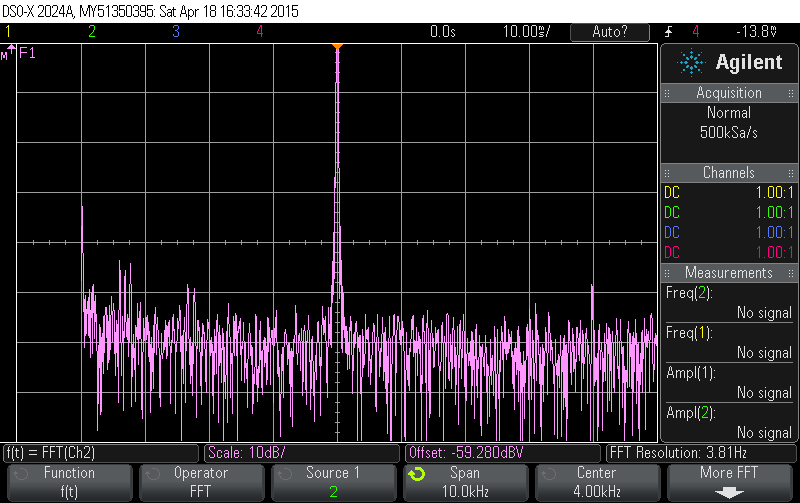
\includegraphics[keepaspectratio=true, scale=0.284]{exps/AE_sem_inter}}
	\hspace{8mm}
	\subfloat[]{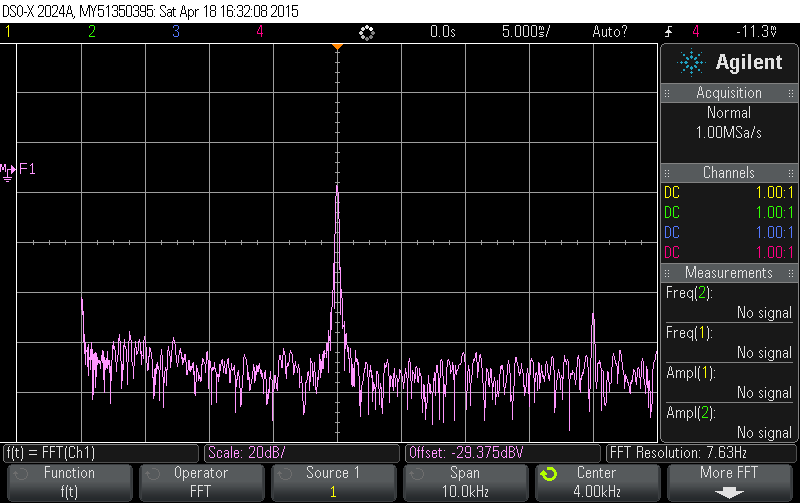
\includegraphics[keepaspectratio=true, scale=0.284]{exps/AE_com_inter}}
	\vspace{-0.8em}
	\caption{Espectro do sinal de saída sem interpolação (a) e com interpolação (b).}
	\vspace{-0.8em}
\end{figure}

Assim, para se poder obter resultados mais conclusivos sobre qual o melhor método recorreu-se ao modo persistência do osciloscópio. Este modo sobrepõe múltiplas formas de onda no mesmo \textit{display}, com as formas de onda mais recentes a serem enfatizadas com uma saturação mais profunda. De referir que para comparar os sinais fixou-se agora o valor de $\Delta$ a 16380, ou seja, uma frequência que não é um múltiplo da frequência de amostragem. Isto é feito porque, quando a frequência é múltiplo da frequência de amostragem, não se ganha nada em implementar o método da interpolação. No entanto, na maioria das vezes a frequência não será múltiplo de $f_s$ e assim, tem-se a ganhar quase sempre. 

Na Figura \ref{fig:AE1} apresenta-se as formas de onda obtidas para as sinusoides geradas de acordo com os dois métodos, com $\Delta$ a 16380.

\begin{figure}[H]
	\centering
	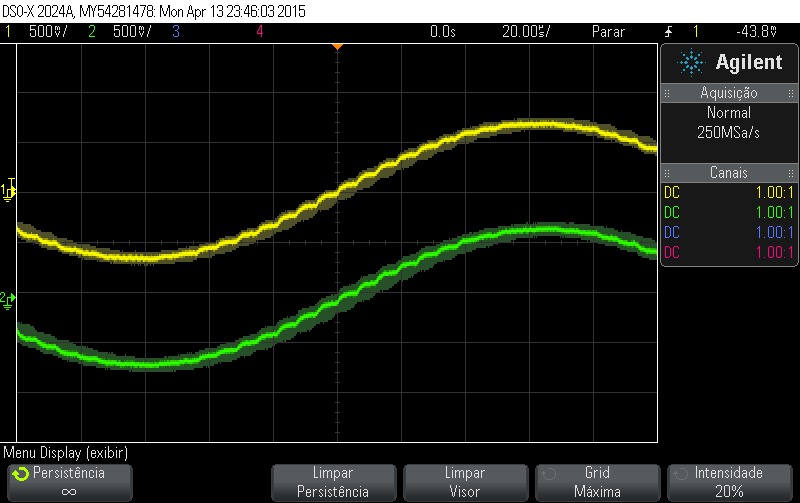
\includegraphics[keepaspectratio=true, scale=0.33]{exps/diferenca1}
	\caption{Onda sinusoidal obtida sem interpolação (a verde) e com interpolação (a amarelo).}
	\vspace{-0.8em}
	\label{fig:AE1}
\end{figure}

Como se pode ver, o sinal representado a verde, implementação sem interpolação, apresenta maior dispersão em torno dos valores pretendidos para a forma de onda. O sinal representado a amarelo, implementação com interpolação, não tem tanta dispersão, estando a gama de valores mais próxima do pretendido. 

Assim se pode concluir que o método da interpolação compensa na maioria das vezes, pois fornece um oscilador de melhor qualidade.

\pagebreak

\section{Projecto $\#$2 - Transmissor BPSK}

Neste projecto, pretende-se implementar o codificador de um transmissor BPSK (\textit{binary phase-shift keying)}, representado na Figura \ref{fig:BPSK}.

\begin{figure}[H]
	\centering
	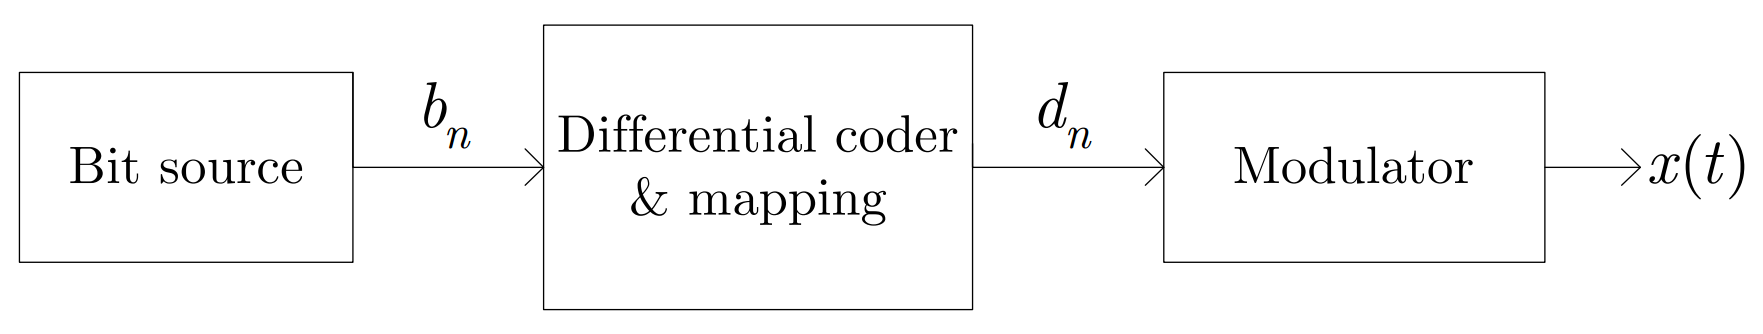
\includegraphics[keepaspectratio=true, scale=0.5]{teoricas/bpsk}
	\caption{Esquema de um transmissor BPSK.}
	\vspace{-0.8em}
	\label{fig:BPSK}
\end{figure}

A modulação BPSK faz o mapeamento de uma mudança na fase de $0\,^{\circ}$ ou $180\,^{\circ}$ para um valor de \textit{bit} de 0 ou 1, respectivamente. Para que não haja ambiguidade na fase, que ocorre quando se utilizam fases absolutas, aplica-se codificação diferencial. Assim, quando o canal introduz uma mudança de fase desconhecida é possível recuperar a sequência de \textit{bits}.

O codificador tem como entrada os \textit{bits} $b_n$, uma sequência que vai alternando entre o valor lógico \texttt{0} e o valor lógico \texttt{1} ($b_n$ = 1, 0, 1, 0, \ldots) e como saída os valores $d_n$, que podem ser -1 ou +1. O codificador realiza a operação $c_n = c_{n-1} \oplus b_n$, considerando $c_0 = 0$, para que depois possam ser determinados os \textit{bits} da sequência $d_n$, de acordo com o mapeamento:

\vspace{-3mm}
\begin{equation}
	c_{n} = 0 \to d_{n} = -1;
	\label{eq:cn0}
\end{equation}
\begin{equation}	
	c_{n} = 1 \to d_{n} = +1.
	\label{eq:cn1}  
\end{equation} 

\vspace{1mm}
Assim, o sinal modulado BPSK é dado por:

\vspace{-3mm}
\begin{equation}
	s(t) = \sin (2 \pi f_0 t + \pi c_n) = d_n \sin (2 \pi f_0 t).
\end{equation} 

Ou, a tempo discreto:

\vspace{-3mm}
\begin{equation}
	s_{n} = s(n T_s) = d_n \sin (2\pi f_0 T_s n).
\end{equation} 

\vspace{1mm}
É utilizada uma frequência de amostragem, $f_s=1/T_s$ , de 16 kHz e uma frequência da portadora, $f_0$, de 4 kHz. A taxa de bits é de $f_b$ = 1 kbps, por isso, por cada \textit{bit}, há 4 períodos da portadora.  

Os \textit{bits} da sequência $b_n$ são implementados recorrendo a um contador, uma vez que a cada 16 amostras do sinal de entrada, é necessário que haja uma alteração do \textit{bit} seguinte da sequência $b_n$, passando de \texttt{0} para \texttt{1} ou vice-versa. Para que seja realizada essa alteração, é utilizada a função \texttt{XOR} do bit $b_n$ anterior com \texttt{1}. Apresenta-se de seguida o excerto de código que implementa a sequência de bits $b_n$. 

\begin{lstlisting}[language=C]
	...
		if(b_i>15){
			b_i=0;
			b_n=(b_n^1); //xor entre valor anterior de bn e o valor logico 1
			...
		}
		b_i++;
	... 
\end{lstlisting}

Foi criada outra solução para a obtenção da sequência $b_n$ com objectivo de não utilizar a instrução condicional, \textit{if}. Seguiu-se o conselho do enunciado de usar um contador que quando ocorre \textit{overflow} gera um novo \textit{bit} alternado. Está representado de seguida no excerto de código:

\begin{lstlisting}[language=C]
	...
		b_i++;			
		b=(b_i&16)>>4;  //mascara para obter o bit de overflow
		b_n=(b_n^b);   //xor para alternar o bit bn
		b_i=(b_i&15); //obtencao dos 4 bits menos significativos
	...
\end{lstlisting}

Como se pode observar, ocorre \textit{overflow} quando o contador, \texttt{b\_i}, atinge o valor 16, sendo utilizado este valor porque a frequência de amostragem, de 16 kHz, é divida por esse valor de forma a obter o resultado desejado de uma taxa de transmissão de 1 kbps. Para detectar esta ocorrência aplica-se a máscara \texttt{16} (o quinto \textit{bit} menos significativo com o valor lógico \texttt{1}) e efectua-se um \textit{shift} de 4 posições para a direita.

\begin{figure}[H]
	\centering
	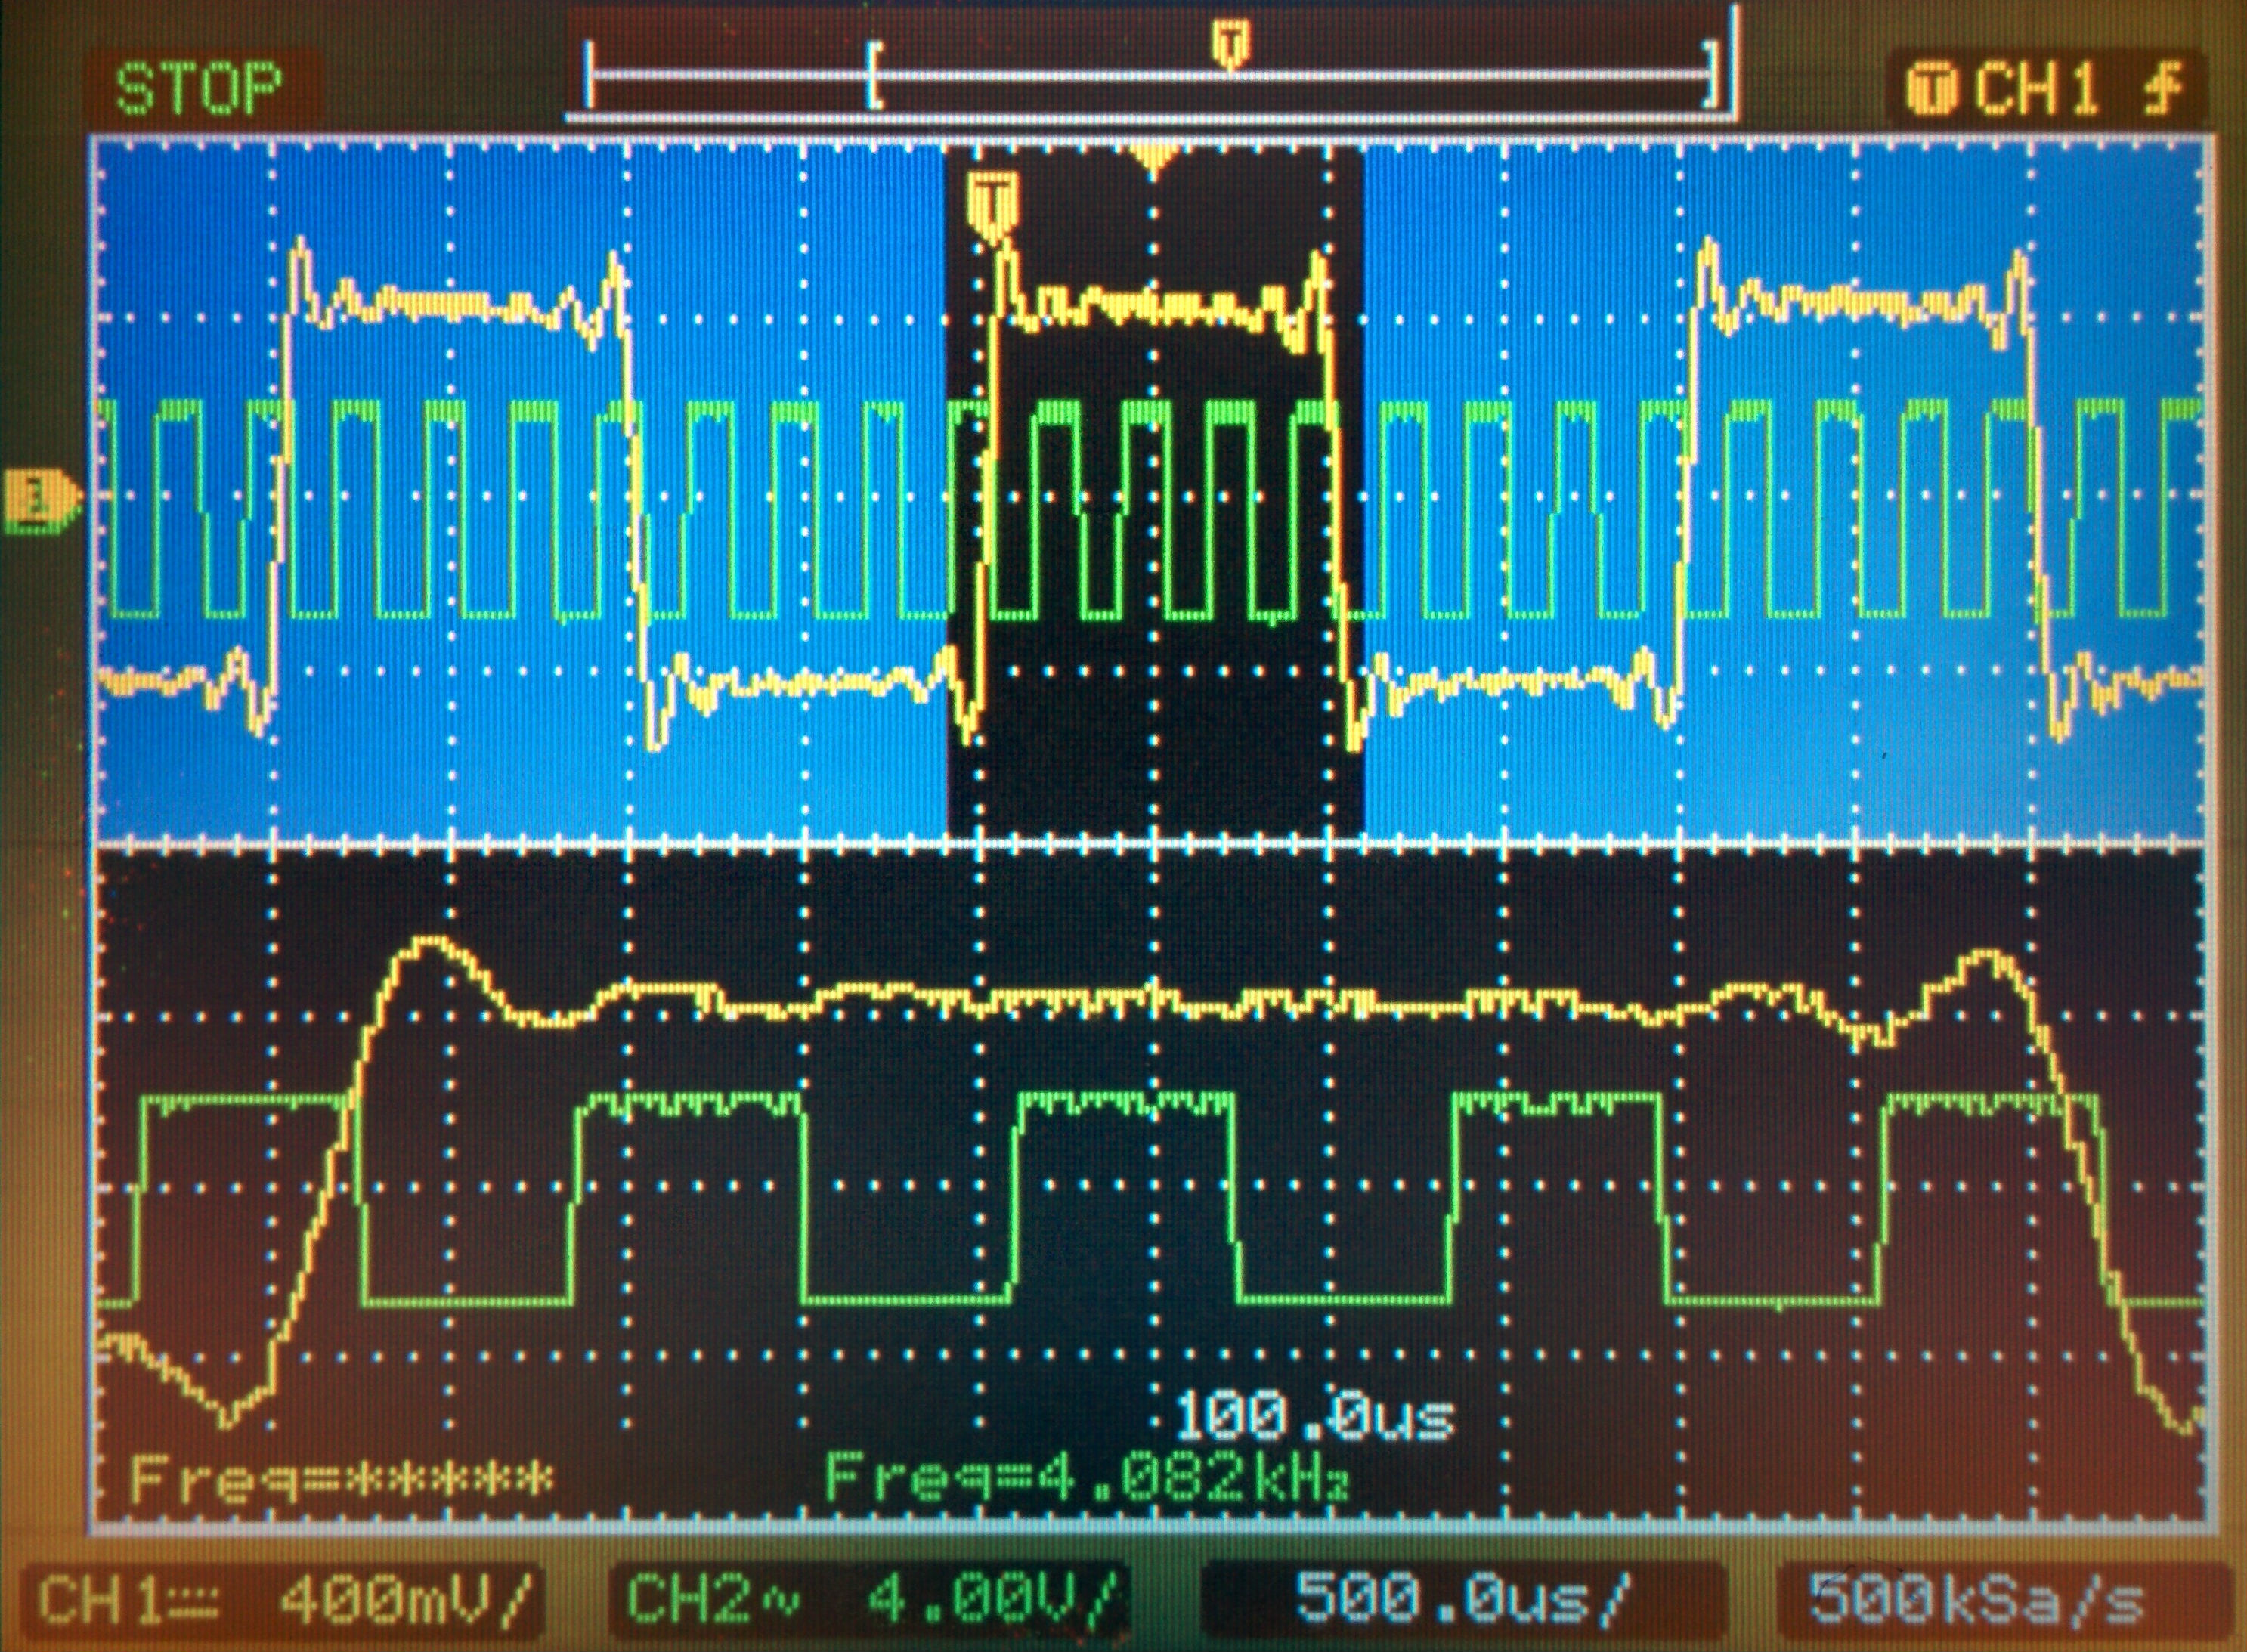
\includegraphics[keepaspectratio=true, scale=0.10]{exps/bn_zoom}
	\caption{Sinal $b_n$ (a amarelo) sobreposto com uma onda quadrada com frequência de 4 kHz (a verde).}
	\vspace{-0.8em}
\end{figure} 

Na figura anterior pode-se analisar o resultado do sinal $b_n$, verificando-se que é um sinal binário, uma vez que só toma o valor 0 ou 1, com um ritmo de transmissão de 1 kbps. Cada \textit{bit} (quando o sinal representado a amarelo toma o valor máximo ou mínimo) contém 4 ciclos da onda quadrada (onda representada a verde que tem uma frequência de 4 kHz), o que resulta numa frequência de \textit{bit} de 4 kHz/4 = 1 kHz. Sabendo que um período do sinal $b_n$ é composto por dois \textit{bits} (valor máximo e mínimo da onda representada a amarelo) conclui-se que se tem um sinal com frequência de 500 Hz, ou seja, 4 kHz/8 = 500 Hz.

\change{o prof diz que nao sabe o que e aquela onda de 4k}

De seguida, aplica-se a função \texttt{XOR} entre o resultado anterior e a variável \texttt{b\_n}, de forma a obter uma sequência $b_n$ que varia alternadamente entre \texttt{0} e \texttt{1}, ou vice-versa, a uma taxa de $f_b$ = 1 kbps. Com o \textit{bit-rate}, $b_n$, criado aplica-se o codificador diferencial de forma a gerar o sinal $c_n$, de acordo com seguinte equação:

\vspace{-3mm}
\begin{equation}
	c_n = c_{n-1} \oplus b_n
\end{equation} 

\vspace{1mm}
A equação anterior foi implementada no ciclo de criação do \textit{bit-rate}, $b_n$,  aplicando a função \texttt{XOR} entre o bit $c_{n-1}$ e $b_n$, como se mostra no seguinte excerto de código:

\begin{lstlisting}[language=C]
	...
		c_n = 0;
		...
		if(b_i>15){
			b_i=0;
			b_n=(b_n^1);
			c_n=c_n^b_n; //codificador diferencial
			...
		}
		b_i++;
	...
\end{lstlisting}
		
De seguida, aplica-se o mapeamento aos \textit{bits} do sinal $c_n$ na constelação BPSK, de forma a obter o sinal $d_n$, ou seja, os dois símbolos da constelação: 1 e $-1$. O mapeamento segue as expressões da equação (\ref{eq:cn0}) e (\ref{eq:cn1}).
	 
A solução computacional mais eficiente que se encontrou consiste em três fases. Na primeira, é efectuado um \textit{shift} de 15 posições para a esquerda, no intuito de o \textit{bit} mais significativo ter o valor do sinal $c_n$. Em segundo, nega-se o vector. E em último, é efectuado um \textit{shift} de 15 posições para a direita. De seguida encontra-se um esquema que demonstra a solução encontrada para a obtenção do $d_n$ como também o código.

\begin{lstlisting}[language=C]
	...
		if(b_i>15){
			...
				c_n = c_n^b_n;
				shift15_cn = c_n<<15;	   // shift de 15 posicoes para a esquerda
				not_shift15 = ~shift15_cn; // negacao do sinal anterior 
				d_n = not_shift15 >>14;    // shift de 14 posicoes para a direita
		}
	...
\end{lstlisting}

\change{rever se compensa o if ou nao - profiling do codigo?}

\begin{figure}[H]
	\centering
	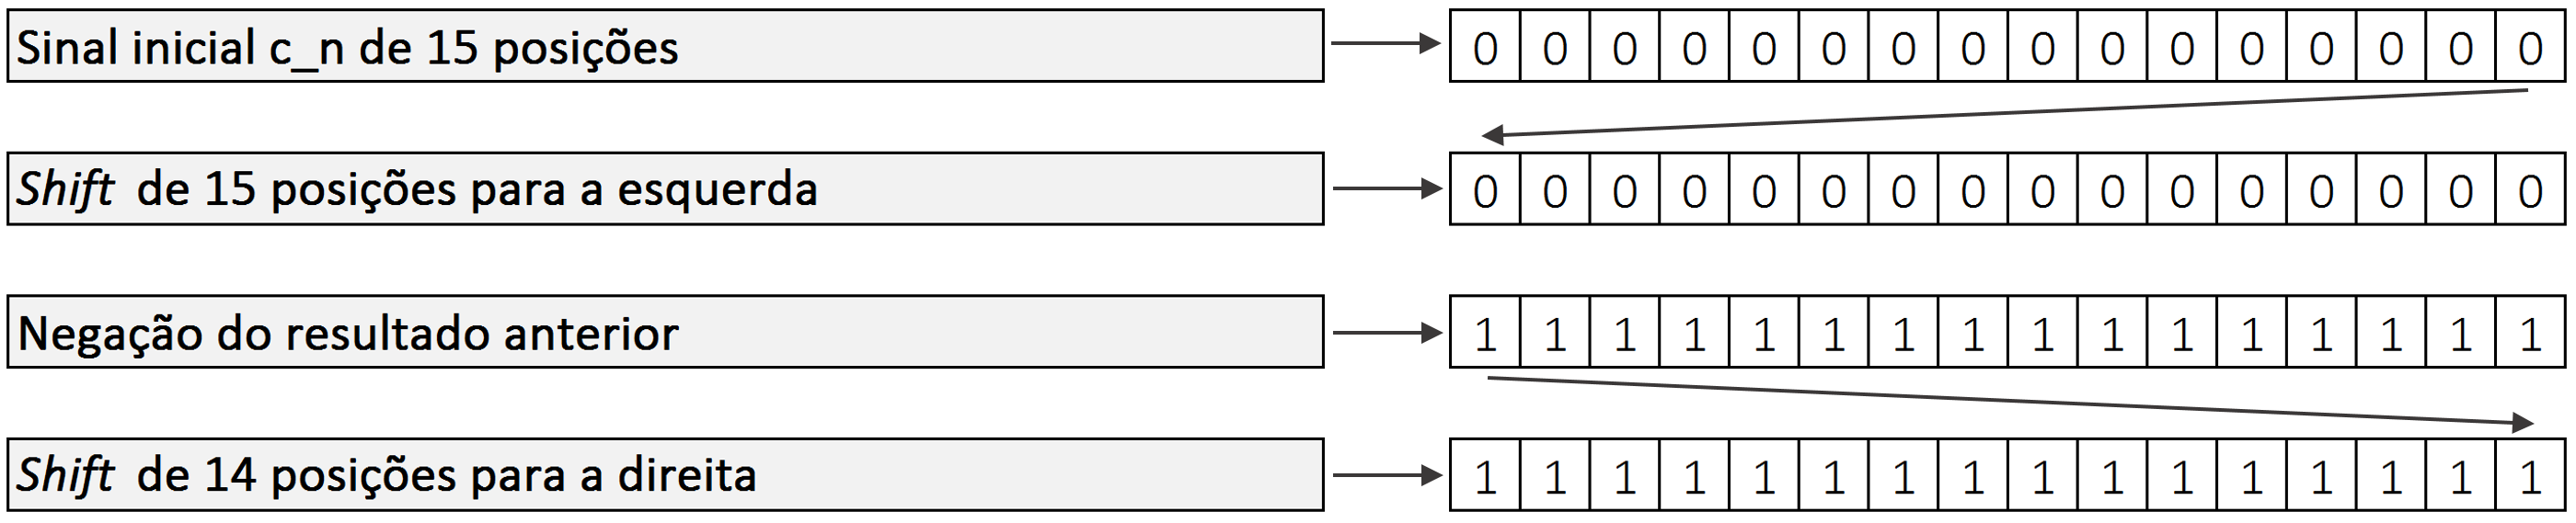
\includegraphics[keepaspectratio=true, scale=0.30]{teoricas/esquema2}
	\caption{Representação da situação em que $c_{n} = 0$, resultando num mapeamento de $d_{n} = -1$.}
	\vspace{-0.8em}
\end{figure}

\begin{figure}[H]
	\centering
	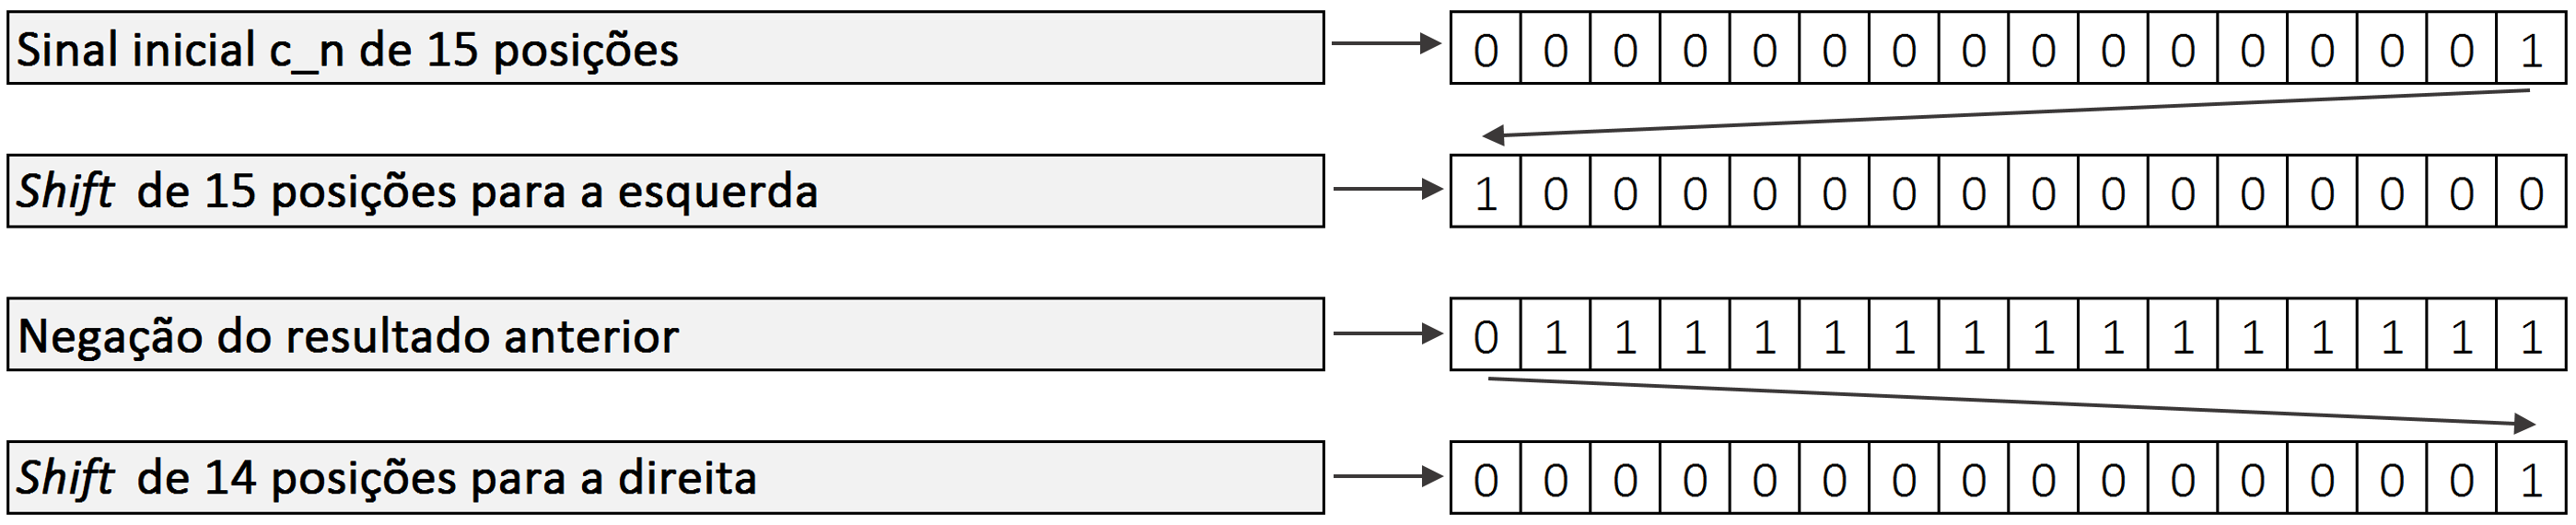
\includegraphics[keepaspectratio=true, scale=0.30]{teoricas/esquema1}
	\caption{Representação da situação em que $c_{n} = 1$, resultando num mapeamento de $d_{n} = +1$.}
	\vspace{-0.8em}
\end{figure}

Pretende-se agora gerar a portadora com frequência $f_0$  a 4 kHz. De forma a implementar a portadora, que vai ser multiplicada pela sequência $d_n$, originando o sinal modulado, é criada uma LUT idêntica à do Projecto \#1. Neste caso, uma vez que só há 4 amostras por período, já que a frequência de amostragem é 
$f_0 = 16$ kHz, basta especificar 4 valores da onda sinusoidal. Assim, é declarada a LUT com os valores 0, 1, 0 e -1, representados no formato mais preciso, $Q_{15}$:

\begin{lstlisting}[language=C]
	...
		//LUT do seno com 4 amostras
		short sine[4] = {0,32767,0,-32767};
	...
\end{lstlisting}

Com a LUT declarada, usou-se o excerto de código seguinte para poder gerar a portadora de frequência $f_0$ a 4 kHz. O código encontra-se no \textit{loop} da rotina principal, de forma a obter um valor da LUT a cada 16 kHz, incrementando a variável de indexação da \textit{look-up-table}, \texttt{sine\_i}, a cada passagem do \textit{loop}. É necessário aplicar a máscara \texttt{3}, os dois \textit{bits} menos significativos a \texttt{1}, para poder aceder às posições 0 a 3 da LUT.

\begin{lstlisting}[language=C]
	while(1){	
		...
			sine_i= sine_i&3; // mascara para obter os 3 bits menos significativos
			y= sine[sine_i];  // indexacao da LUT
			sine_i++;		  // incrementador do index
		...
	}
\end{lstlisting}

Com a primeira parte do modulador criado, geração da portadora, pode-se aplicar a fase final do seu desenvolvimento, a multiplicação do sinal $d_n$ com a portadora, gerando assim um sinal modelado do tipo BPSK. O código seguinte demonstra esta última fase.  

\begin{lstlisting}[language=C]
	 ...
		 y = d_n*y; // multiplicacao do sinal com a portadora
		 AIC_buffer.channel[LEFT] = y;// sinal observado no canal esquerdo
	 ...
\end{lstlisting}

Com o modulador criado procede-se à fase de testes. Sabe-se que o sinal $d_n$ tem uma frequência de 500 Hz com um ritmo de transmissão de 1 kbps, e é modulado por uma portadora de 4 kHz. Assim, existe uma inversão de fase a cada 4000/500 ciclos, ou seja, a cada 8 ciclos.

Analisando a figuras seguinte verifica-se que o modulador está a funcionar correctamente, invertendo a fase no zero da portadora e a cada 8 ciclos.

\begin{figure}[H]
	\centering
	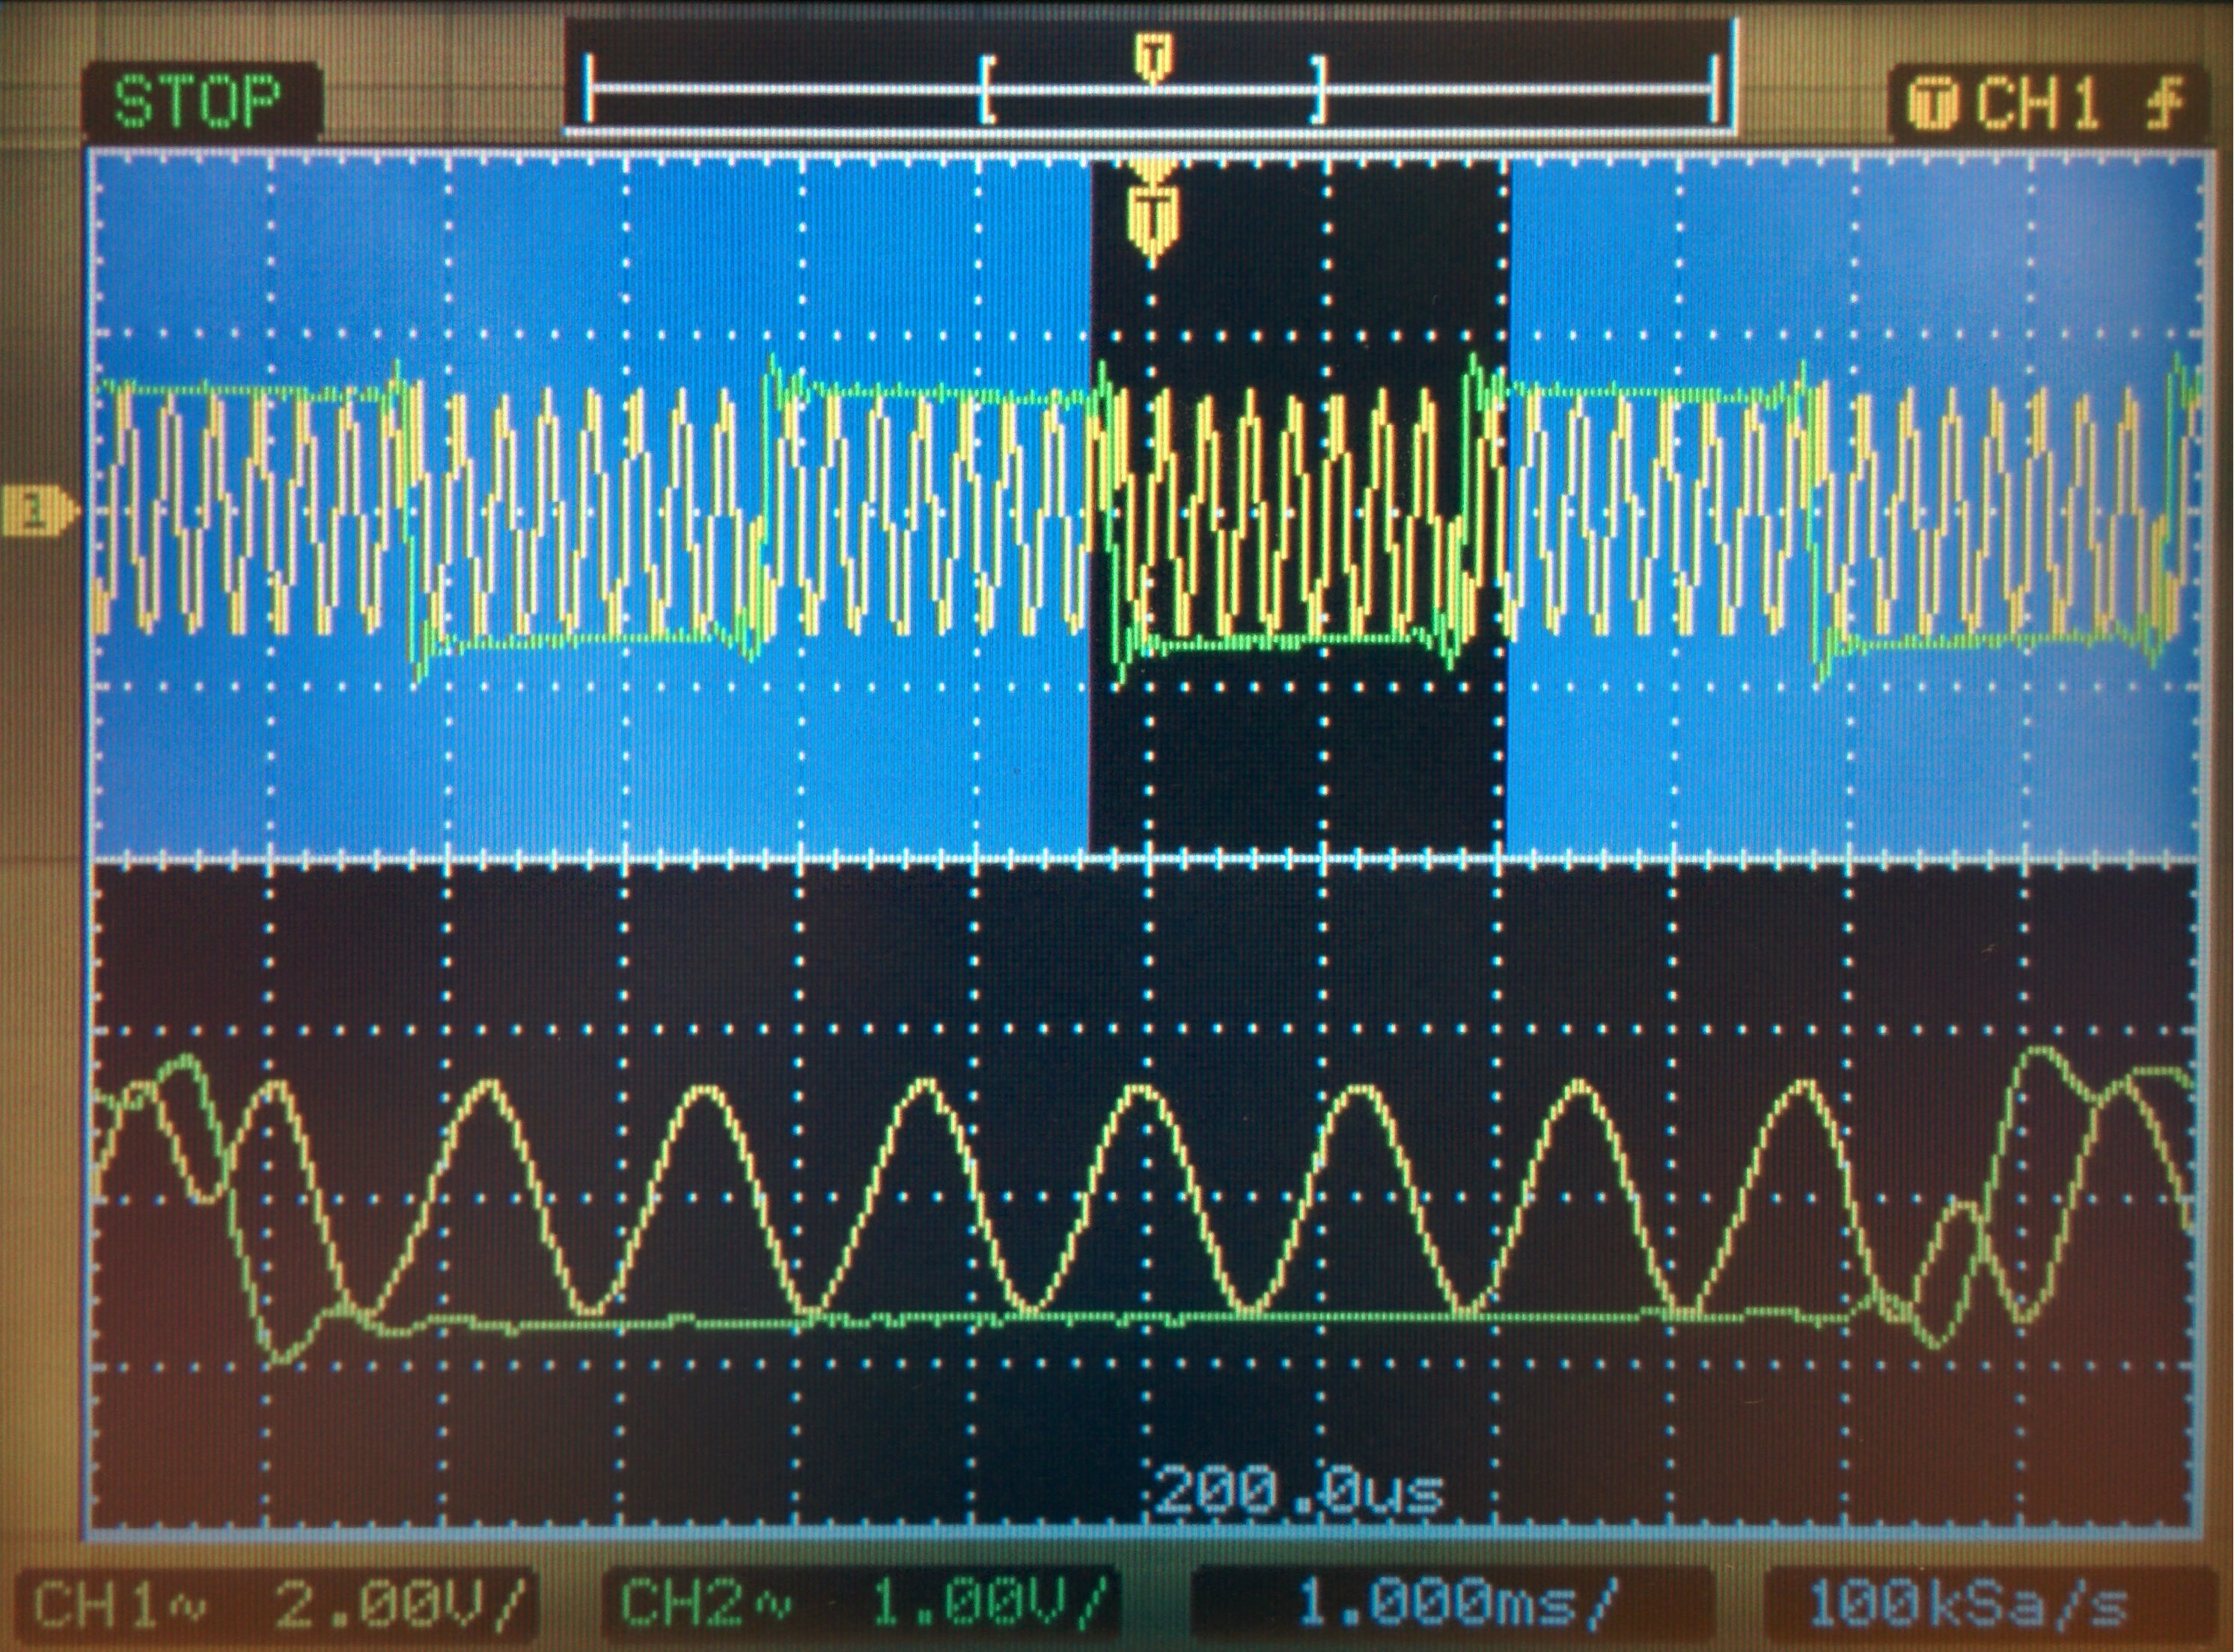
\includegraphics[keepaspectratio=true, scale=0.10]{exps/dn_com_y}
	\caption{Sobreposição do sinal modulado (a amarelo) com o sinal $d_n$ (a verde).}
	\vspace{-0.8em}
\end{figure}

Na figura anterior, pode-se verificar que a inversão de fase faz-se correctamente - quando o sinal $d_n$ passa de $+1$ para $-1$ a inversão é feita para a arcada positiva, como se pode verificar do lado esquerdo da figura. Quando o sinal $d_n$ passa de $-1$ para $+1$ a inversão é feita para a arcada negativa, como se pode verificar na inversão do lado direito da figura.

Apresenta-se também uma imagem em que se encontra apenas representado o sinal modulado, com um \textit{zoom} sobre uma altura em que ocorrem duas inversões de fase. 

\begin{figure}[H]
	\centering
	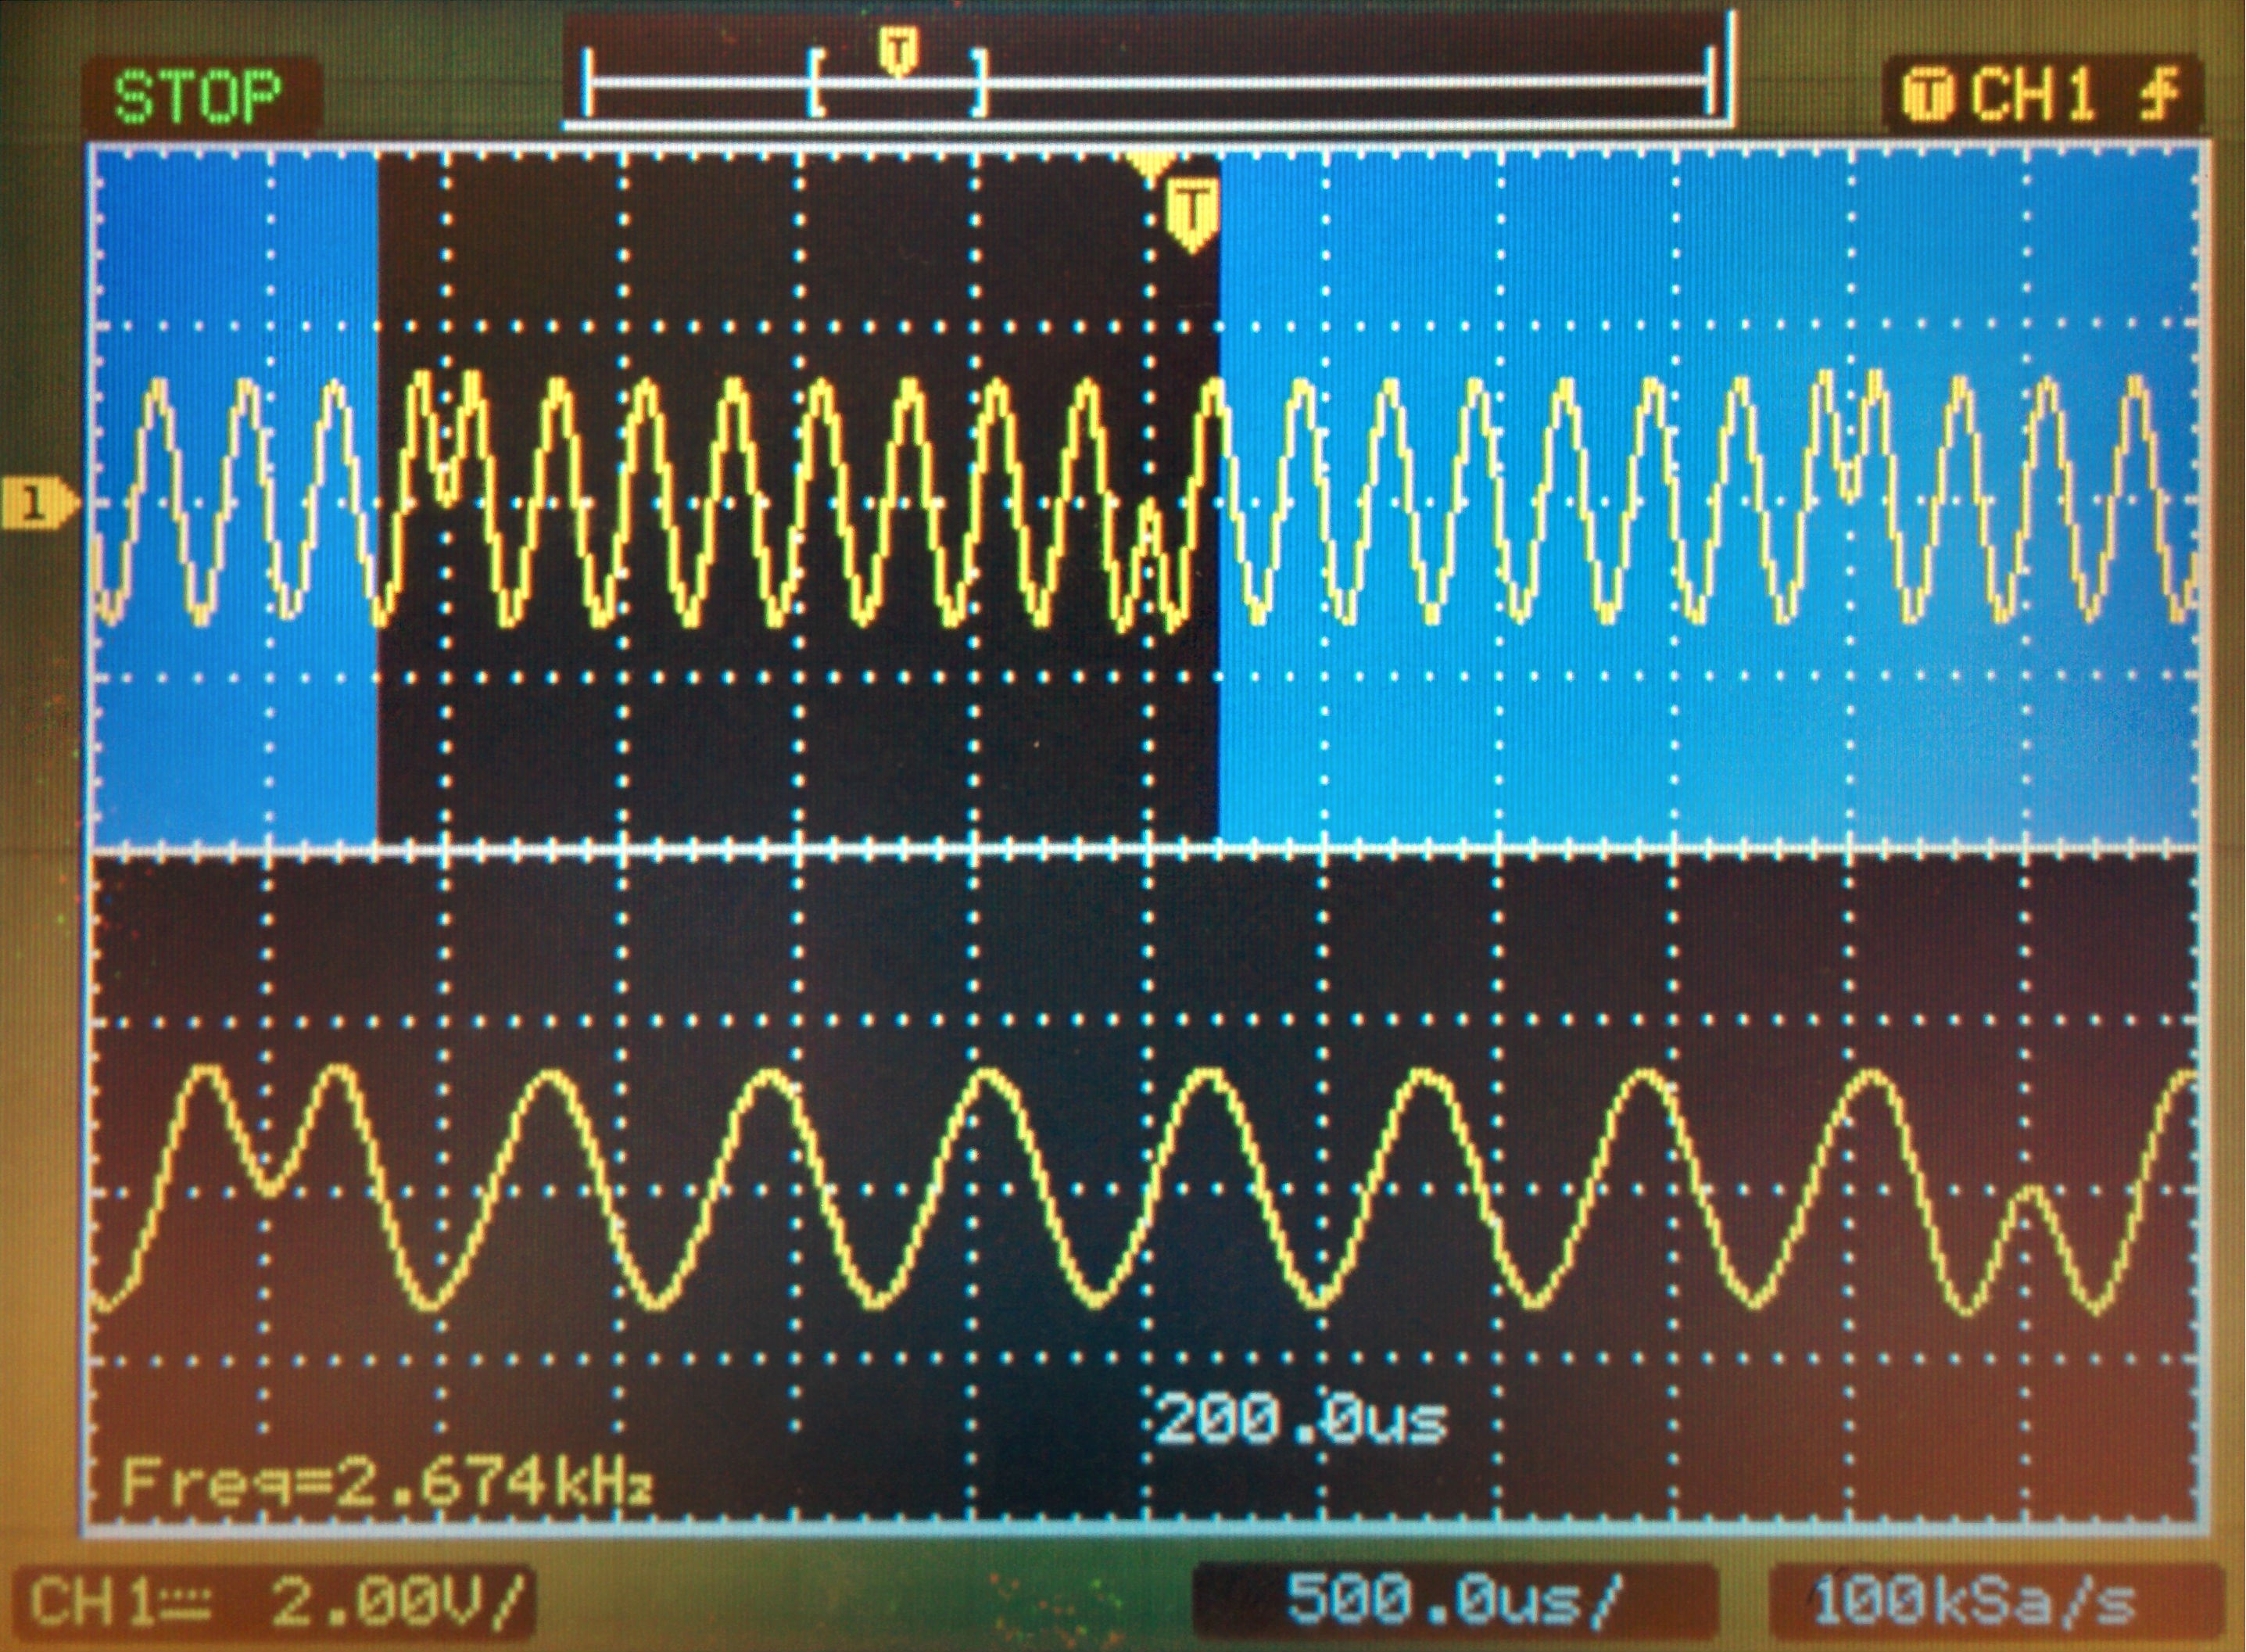
\includegraphics[keepaspectratio=true, scale=0.10]{exps/BPSK_modulated}
	\caption{Sinal modulado (em cima) e pormenor obtido com recurso a uma janela temporal (em baixo).}
	\vspace{-0.8em}
\end{figure}

Efectuou-se também um registo ao nível de espectros para vários sinais, como se pode ver nas figuras da próxima página.

\begin{figure}[H]
	\centering
	\subfloat[]{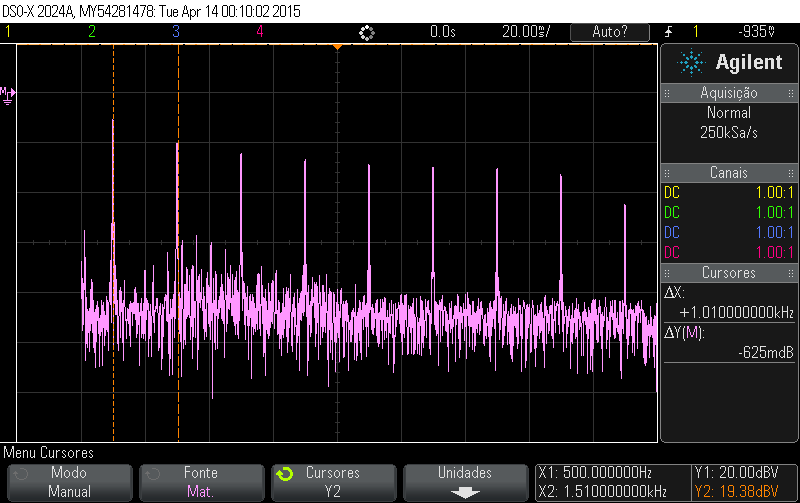
\includegraphics[keepaspectratio=true, scale=0.284]{exps/AE_bn}}
	\hspace{8mm}
	\subfloat[]{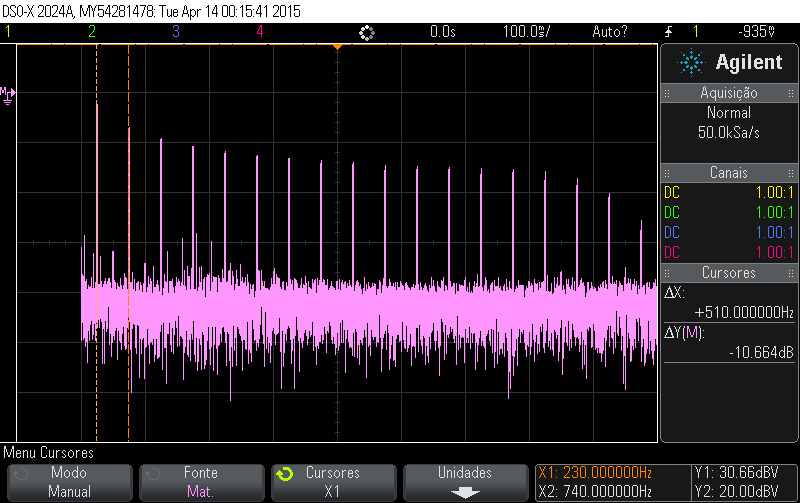
\includegraphics[keepaspectratio=true, scale=0.284]{exps/AE_dn}}
	\linebreak
	\subfloat[]{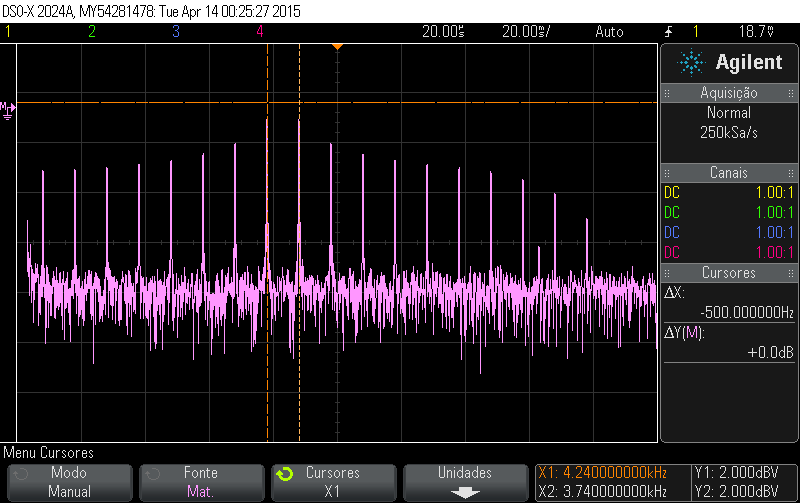
\includegraphics[keepaspectratio=true, scale=0.284]{exps/AE_yn}}
	\vspace{-0.8em}
	\caption{Espectro do sinal $b_n$ (a), espectro do sinal $d_n$ (b) e espectro do sinal $y_n$ (c).}
	\vspace{-0.8em}
\end{figure}

Relativamente ao espectro do sinal $b_n$ verifica-se que existe uma risca na frequência de 500 Hz, e também em 1500 Hz, 2500 Hz, e por aí adiante, com um intervalo entre riscas de 1 kHz. Isto deve-se ao facto de o ritmo de transmissão dos \textit{bits} ser de 1 kbps e a sequência ser alternada. Perante estas condições tem-se uma onda quadrada com 500 Hz de frequência. O espectro do sinal $b_n$ representa a informação do \textit{bit} com valor lógico 1, enquanto o espectro de $d_n$ representa a informação resultante do mapeamento do \textit{bit} com valor lógico 1 e $-1$. 

O espectro de $y_n$ permite verificar o fenómeno de modulação, na medida em que se verifica que o espectro de $d_n$ foi deslocado para altas frequências, ou seja, encontra-se em torno do espectro da portadora que corresponde a uma risca na frequência $f_0$, 4 kHz. De facto, ocorre a convolução do espectro do sinal $d_n$ com o espectro da portadora.

Analisando agora a Figura 1 verifica-se que do transmissor BPSK ainda falta implementar o módulo de \textit{scrambler}. Nesta altura do desenvolvimento do projecto já estão implementados os módulos de geração de \textit{bits}, de codificação diferencial e de modulação, estando o sinal BPSK, $x\left(t\right)$, disponível.

A geração de \textit{bits} que se implementou é, no fundo, um simples gerador de uma sequência de \textit{bits} bem definida ($b_n$ = 1, 0, 1, 0, \ldots). No entanto, esta sequência não é apropriada para transmissão e, como tal, a sequência referida anteriormente necessita de ser ``misturada'' de modos a que surja de forma aleatória. Para se efectuar isto recorre-se a um circuito denominado de \textit{scrambler}.

O \textit{scrambler} é um dispositivo que inverte a ordem e polaridade dos \textit{bits} da mensagem a ser enviada. A utilização deste dispositivo tem dois principais objectivos, a facilidade de execução dos circuitos de recuperação de relógio, \textit{clock and data recovery},e outros circuitos adaptativos do receptor. Esta melhoria deve-se ao facto do \textit{scambler} eliminar longas sequências constantes de \texttt{0} ou \texttt{1} O outro objectivo deve-se ao facto de eliminar a dependência do sinal a ser transmitido no espectro de potência, ou seja, o sinal transmitido fica mais disperso de forma a maximizar os requisitos do espectro de potência. Pois se a potência for concentrada numa largura de banda limitada pode haver interferência nos canais adjacentes do receptor devido à intermodulação, este fenómeno é conhecido por \textit{cross-modulation}.

O circuito do dispositivo \textit{scrambler} tem como expressão matemática o polinómio seguinte:
\begin{equation}
	P(x)~= ~1~+~x^{-6}~+~x^{-7}
\end{equation}  

Os valores de $x^{-6}$ e $x^{-7}$ representam o sinal de entrada com um atraso de 6 e 7 períodos respectivamente, a implementação do circuito segue o seguinte esquema:

\begin{figure}[H]
	\centering
	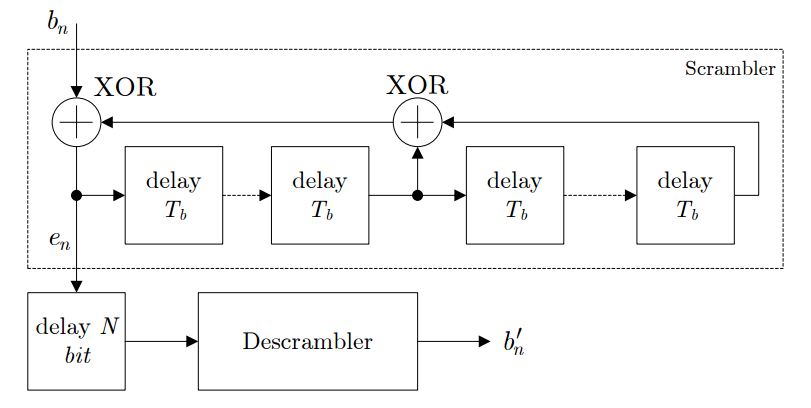
\includegraphics[keepaspectratio=true, scale=0.50]{teoricas/scrambler}
	\caption{Esquema da implementação do \textit{scrambler}.}
	\vspace{-0.8em}
\end{figure}

Analisando o esquema proposto efectuou-se a implementação do circuito na DSP com o apoio do código C.
Começou-se por definir uma variável de 8 \textit{bits}, \texttt{char delay\_scrambler} que guarda os atrasos temporais de até 7 períodos. O código seguinte demonstra a implementação e obtenção dos atrasos necessários para o \textit{scrambler}. É de referir que onde o sinal de entrada consiste na sequência de \textit{bits} \texttt{b\_n} gerada anteriormente:

\begin{lstlisting}[language=C]
		...
	 unsigned char delay_scrambler=0,...;
	 ...
		delay_scrambler = (delay_scrambler>>1)&0x7f;/*Deslocamento temporal*/
		delay_scrambler = delay_scrambler | (e_n<<7);/*Actualizacao do novo valor de e_n no vector*/	
	...
\end{lstlisting}

Assim sendo o \textit{bit} mais significativo representado o resultado do \textit{scrambler} com atraso \texttt{0} e por consequente o \textit{bit} menos significativo representa o atraso 7 na linha temporal. Seguindo esta lógica o vector \texttt{delay\_scrambler} é actualizado da seguinte forma:

\begin{figure}[H]
	\centering
	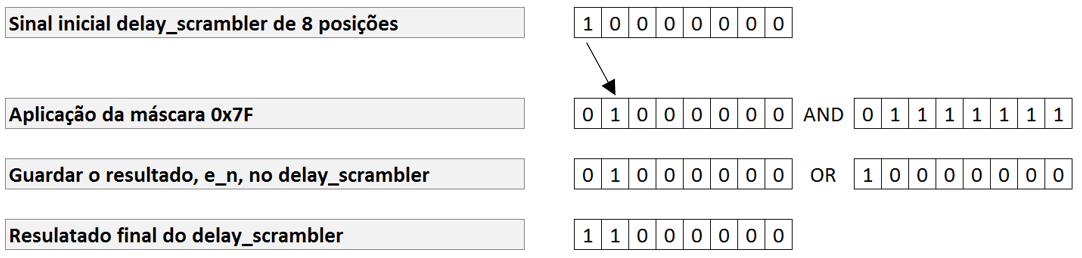
\includegraphics[keepaspectratio=true, scale=0.40]{teoricas/calculodoscrambler}
	\caption{Esquema do cálculo do \texttt{delay\_scrambler}.}
	\vspace{-0.8em}
\end{figure}
Inicialmente é realizado um \textit{shift} de uma posição para direita no vector \texttt{delay\_scrambler}, representando o deslocamento temporal de cada amostra. De seguida aplica-se a máscara \texttt{0x7f} de forma a obter um \texttt{0} no \textit{bit} mais significativo e mantendo os valores das amostras deslocadas. Com o deslocamento feito recorre-se à operação lógica OR para guardar o resultado do \textit{scrambler} no atraso temporal \texttt{0}.

Com a actualização do vector \texttt{dela\_scarmbler} realizada a obtenção do resultado do \textit{scrambler} é obtida da seguinte forma:  

\begin{figure}[H]
	\centering
	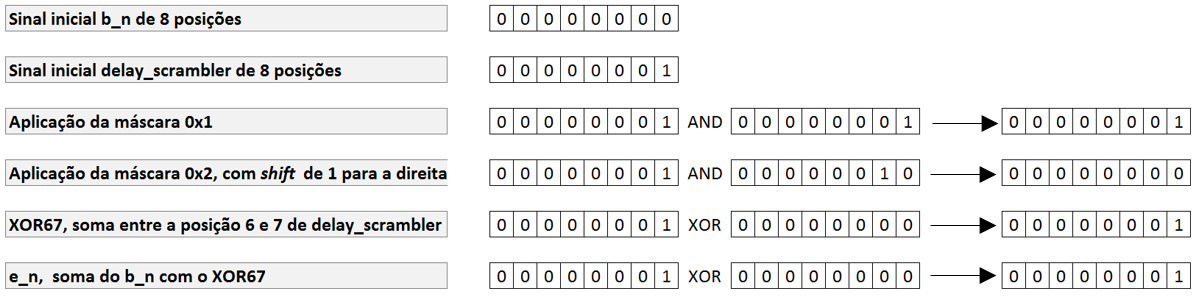
\includegraphics[keepaspectratio=true, scale=0.40]{teoricas/calculodeen}
	\caption{Esquema do cálculo da saída do \texttt{scrambler}.}
	\vspace{-0.8em}
\end{figure}

Começa-se por somar os resultados do \textit{scrambler} referente ao atraso 6 e 7 guardando em \texttt{Xor67}. E seguida soma-se com \texttt{b\_n} originando o \texttt{e\_n}. A implementação em código segue no excerto seguinte:

\begin{lstlisting}[language=C]
	...
	short     b_i_TX = 1,...;
	short     ..., e_n=0, xor67=0;
	short     b_n = 1,..;
	unsigned char delay_scrambler=0,...;
	...
		 if(b_i_TX>15){
			b_i_TX = 0;
			b_n = (b_n^1);
			 
			/*Scrambler*/
			xor67 = (delay_scrambler&1)^((delay_scrambler&2)>>1);
			e_n = b_n^xor67;
			delay_scrambler = (delay_scrambler>>1)&0x7f;/*Deslocamento temporal*/
			delay_scrambler = delay_scrambler | (e_n<<7);/*Actualizacao do novo valor de e_n no vector*/
			...
		}
		b_i_TX	
	...
\end{lstlisting}

A imagem seguinte representa a visualização do sinal de saída do \textit{scrambler} como também do sinal \texttt{b\_n}: 

\begin{figure}[H]
	\centering
	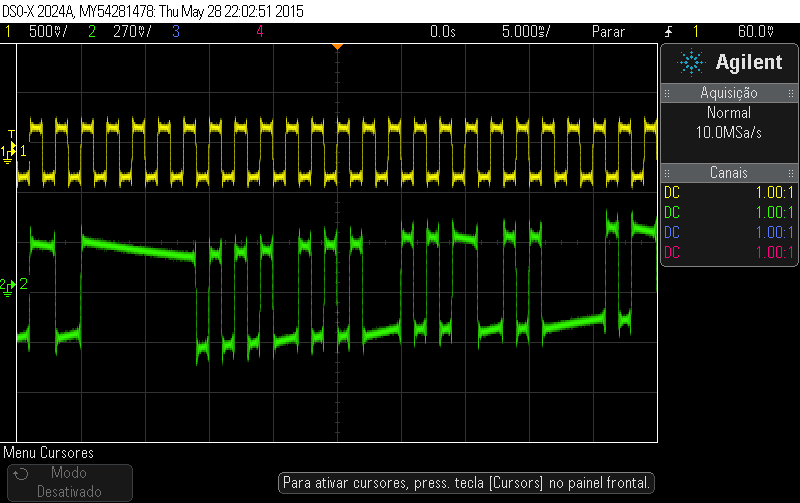
\includegraphics[keepaspectratio=true, scale=0.40]{exps/ScramblerBnVsEn}
	\caption{Imagem do  sinal \texttt{b\_n}, sinal a amarelo, e do sinal \texttt{e\_n}, sinal a verde.}
	\vspace{-0.8em}
\end{figure}

Como se pode observar, a implementação do \textit{scrambler} foi bem sucedida devido à aleatoriedade da sequência de \textit{bits} obtida, visualizar o sinal a verde. 


\section{Projecto $\#$3 - Receptor BPSK}

DESCRAMBLER


COSTAS LOOP

\todo{1 - teddy}

\todo{2 e 3 - david - nas imagens e bom tirar a LB, para comprovar que esta a funcionar}

O modem BPSK, apresentado na Figura 2, é constituído por vários módulos, sendo que três desses módulos tratam-se de filtros passa-baixo. Esses filtros apresentam um pólo e um zero, satisfazendo a seguinte equação às diferenças:

\vspace{-3mm}
\begin{equation}
y(n) = \alpha y(n-1) + \gamma \frac{1-\alpha}{1-\beta}[x(n)-\beta x(n-1)],
\end{equation} 

\vspace{1mm}
que apresentam um diagrama de fluxo de sinal como o apresentado na Figura \ref{fig:fluxo}.

\begin{figure}[H]
	\centering
	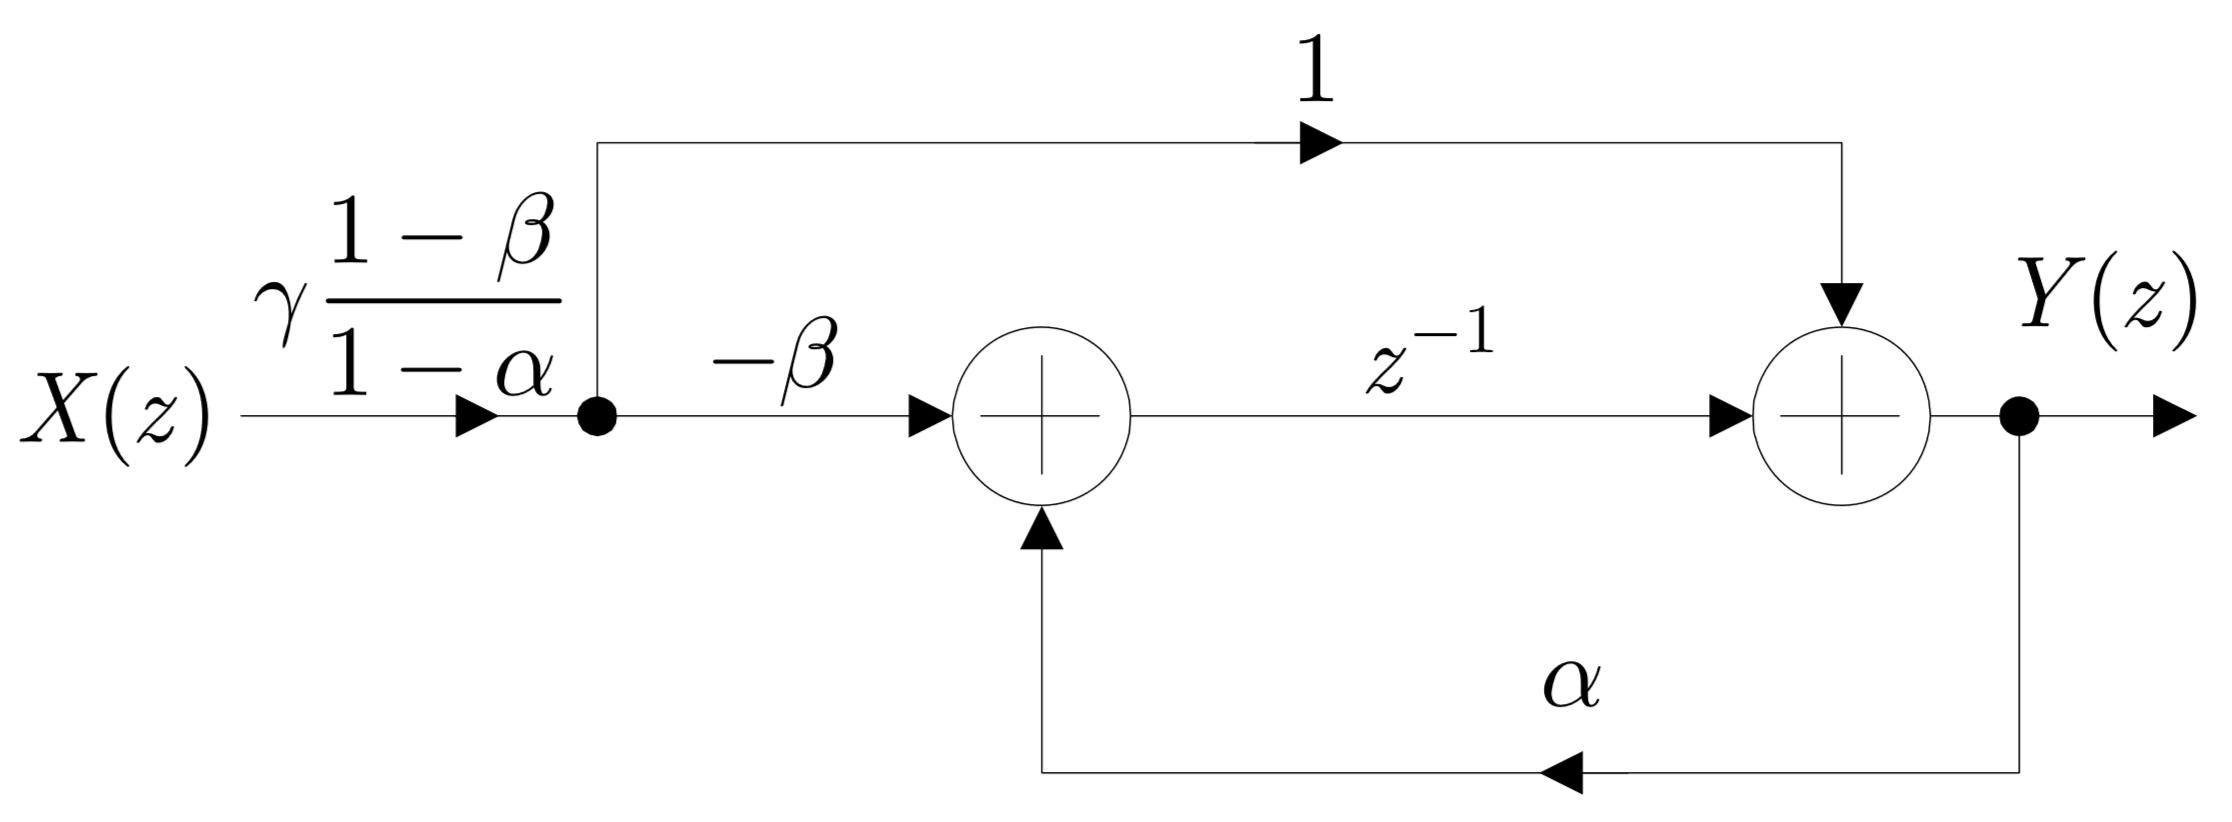
\includegraphics[keepaspectratio=true, scale=0.20]{teoricas/diagrama_fluxo}
	\caption{Diagrama de fluxo de sinal de filtro passa-baixo.}
	\label{fig:fluxo}
	\vspace{-0.8em}
\end{figure}

Aplicando a transformada Z, é possível determinar a função de transferência do filtro, obtendo-se:

\vspace{-3mm}
\begin{equation}
H(z) = \frac{\gamma \frac{1-\alpha}{1-\beta} (1-\beta z^{-1})}{1-\alpha z^{-1}}.
\end{equation}
 
\vspace{1mm}
Neste caso, considera-se $\beta=0$, resultando uma expressão mais simples para a função de transferência:
 
\vspace{-3mm}
\begin{equation}
H(z) = \frac{\gamma(1-\alpha)}{1-\alpha z^{-1}}.
\end{equation} 

\vspace{1mm}
Após a determinação da função de transferência geral, para o caso em que $\beta = 0$, é necessário calcular as constantes $\alpha$ e $\gamma$ para os dois tipos de filtros presentes no \textit{Costas Loop}, que apesar de serem ambos filtros passa-baixo, apresentam frequências de corte diferentes, sendo que o ganho DC é igual nos dois casos. As especificações dos dois tipos de filtros, \textit{data filter} e \textit{loop filter}, sendo que existem dois filtros do primeiro tipo e apenas um do segundo, são apresentadas na Tabela 3. 

\begin{table}[H]
 	\centering
 	\caption{Especificações dos filtros passa-baixo.}
 	\vspace{-1.5mm}
 	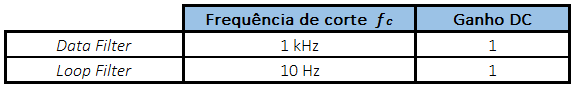
\includegraphics[keepaspectratio=true, scale=0.35]{tabelas/especificacoes}
\end{table}

Sabendo que o ganho DC é igual em todos os filtros, é possível determinar o valor de $\gamma$ dos mesmos, tendo em conta que em DC se tem $\omega = 0$, portanto:

\vspace{-3mm}
\begin{equation}
	z = e^{j \omega T_s} = 1.
\end{equation}

\vspace{1mm}
De onde vem:

\vspace{-3mm}
\begin{equation}
	H(z = 1) = \frac{\gamma(1-\alpha)}{1-\alpha} \longrightarrow \gamma = 1.
\end{equation} 

\vspace{1mm}
Sabe-se, à \textit{priori}, analisando a função de transferência H(z), já com $\gamma = 1$, que o valor de $\alpha$ tem que estar compreendido entre -1 e 1 para o filtro ser estável, sendo que esse valor, para o filtro ser passa-baixo, tem que estar definido entre 0 e 1. Mais ainda, esse valor vai ser diferente para os dois tipos de filtros, visto que o mesmo é determinado em função da frequência de corte, \textit{$f_c$}. Recorrendo à expressão do ganho do filtro vem:

\vspace{-3mm}
\begin{equation}
	|H(j\omega)| = \frac{1-\alpha}{|1-\alpha e^{j\omega T_s}|},
\end{equation} 

\vspace{1mm}
em que é possível particulizar o valor do ganho do filtro à frequência de corte:

\vspace{-3mm}
\begin{equation}
	|H(j\omega_c)| = \frac{1-\alpha}{|1-\alpha e^{j\omega_c T_s}|} = \frac{1 - \alpha}{\sqrt{1- \alpha^2 cos^2{(\omega_c T_s)} + \alpha^2 sen^2{(\omega_c T_s)}}},
\end{equation} 

\vspace{1mm}
de onde se poderia retirar o valor de $\alpha$, o que envolveria alguma manipulação algébrica. No entanto, sabendo que a frequência de corte dos filtros é muito inferior ao valor da frequência de amostragem dividido por 2, $f_s/2$, vem que:

\vspace{-3mm}
\begin{equation}
\omega_ c T_s = 2\pi \frac{f_c}{f_s} \ll 1,
\end{equation} 

\vspace{1mm}
podendo considerar-se a seguinte aproximação:

\vspace{-3mm}
\begin{equation}
e^{-j\omega T_s} \approx 1 - j\omega_c T_s,
\end{equation} 

\vspace{1mm}
resultando então uma expressão para o ganho do filtro, à frequência de corte, bastante mais simples:

\vspace{-3mm}
\begin{equation}
|H(j\omega_c)| =  \frac{1 - \alpha}{|1-\alpha(1-j\omega_c T_s)|},
\end{equation} 

\vspace{1mm}
resultando, finalmente:

\vspace{-3mm}
\begin{equation}
\omega_c = \frac{1 - \alpha}{\alpha T_s} = \frac{1 - \alpha}{\alpha} f_s
\end{equation} 

\vspace{1mm}
Assim, tendo em conta que $f_s = 16$ kHz, pode-se calcular o valor de $\alpha$ para os filtros \textit{data} e filtro \textit{loop}. Sabendo que o valor vai estar contido no intervalo $]0,1[$, pode-se utilizar a representação numérica mais precisa $Q_{15}$ para representar o valor de $\alpha$, de forma a efectuar a implementação dos filtros. Na tabela seguinte, são apresentados os valores de $\alpha$ e também a sua conversão em $Q_{15}$.

\begin{table}[H]
	\centering
	\caption{Valores de $\alpha$ dos filtros passa-baixo.}
	\vspace{-1.5mm}
	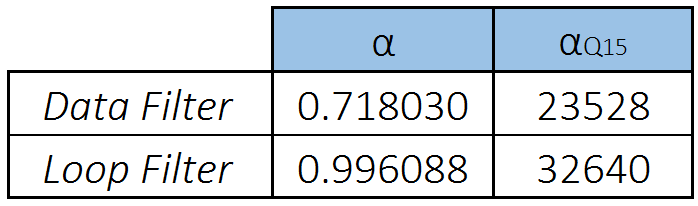
\includegraphics[keepaspectratio=true, scale=0.35]{tabelas/alphas}
\end{table}

Assim, conhecendo-se todos os parâmetros das funções de transferência dos filtros, é possível implementar os filtros, segundo a equação às diferenças:

\vspace{-3mm}
\begin{equation}
y(n) = \alpha y(n-1) +  (1-\alpha)x(n)
\end{equation} 

sendo que um dos filtros \textit{Data} tem como entrada o sinal resultante da multiplicação entre o sinal BPSK e o sinal $\cos(2\pi f_0 + \phi_0)$ e o outro tem como entrada o sinal resultante da multiplicação entre o sinal BPSK e o sinal $\sin(2\pi f_0 + \phi_0)$. De seguida, é apresentado o excerto de código que permite implementar os filtros. 

\begin{lstlisting}[language=C]
short x_cos = 0, x_sine = 0, y_cos_datafilter = 0, y_sin_datafilter = 0;  short in_loopfilter = 0, y_loop filter = 0, alpha_1k = 23528; 
short alpha_10 = 32640, um_menos_alpha_1k = 9240, um_menos_alpha_10 = 127;

...
 //Data Filter
 x_cos = ((xt_bpsk*y_cos)<<1)>>16;
 x_sine = ((xt_bpsk*y_sin)<<1)>>16;
 y_cos_datafilter=(((alpha_1k*y_cos_datafilter)<<1)+((x_cos*um_menos_alpha_1k)<<1))>>16;
 y_sin_datafilter=(((alpha_1k*y_sin_datafilter)<<1)+((x_sine*um_menos_alpha_1k)<<1))>>16;

 //Loop Filter
 in_loopfilter = ((y_cos_datafilter*y_sin_datafilter)<<1)>>16;
 y_loopfilter = (((alpha_10*y_loopfilter)<<1)+ ((in_loopfilter*um_menos_alpha_10)<<1))>>16;
...

\end{lstlisting}
\todo{apresentar código de uma forma melhor}

No entanto, antes de ligar todo o sistema, é importante testar o filtro que tem frequência de corte de $f_c = 1 kHz$, pondo à entrada do mesmo um sinal proveniente do gerador de sinais, de forma a comprovar o correcto funcionamento do filtro, não sendo possível testar o filtro com frequência de corte de 10 Hz, já que à entrada da placa se encontra impossível, o que torna impossível verificar que a implementação do \textit{Loop Filter} está correcta. Assim, para o filtro \textit{Data}, visualizou-se a saída do mesmo, apresentada na Figura X, com um sinal de entrada sinusoidal de 250 Hz, de forma a verificar o ganho em baixas frequências.

\begin{figure}[H]
	\centering
	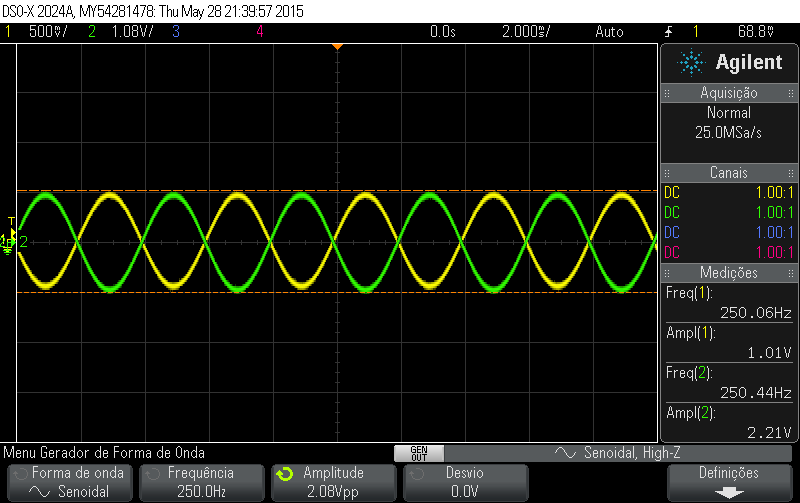
\includegraphics[keepaspectratio=true, scale=0.37]{exps/filtro_1k_baixafreq}
	\caption{Verificação do ganho em baixas frequências - sinal de entrada (a verde) e sinal de saída (a amarelo) do filtro \textit{data}.}
	\vspace{-0.8em}
\end{figure} 

Analisando os valores de amplitude dos dois sinais, pode verificar-se que o ganho é de, aproximadamente, $1/2$, não correspondendo ao ganho unitário pretendido, o que se deve ao facto da placa introduzir um factor de ganho que faz com que o sinal de saída do filtro tenha um ganho inferior a 1. 
Testou-se ainda a frequência de corte, sendo que para isso aumentou-se a frequência do sinal de entrada até o sinal de saída do filtro apresentar uma queda de 3 dB, ou seja, tendo o ganho em baixa frequência o valor de 1.01 V, pretende-se registar a frequência a que o filtro apresenta no sinal de saída um valor de, aproximadamente, 0.7 V.

\vspace{-3mm}
\begin{equation}
	|H(j\omega_{-3dB})| = \frac{|H(j\omega \approx 0)|}{\sqrt{2}} = \frac{1}{\sqrt{2}} \approx 0.7 V
\end{equation} 

Verificou-se, como se pode observar na Figura X, que a frequência de corte apresentava o valor de 963 Hz, o que se trata de um valor próximo de 1 kHz. A pequena diferença em relação ao valor pretendido pode dever-se a se ter registado uma frequência onde ainda não tinham caído exactamente os 3 dB.

\begin{figure}[H]
	\centering
	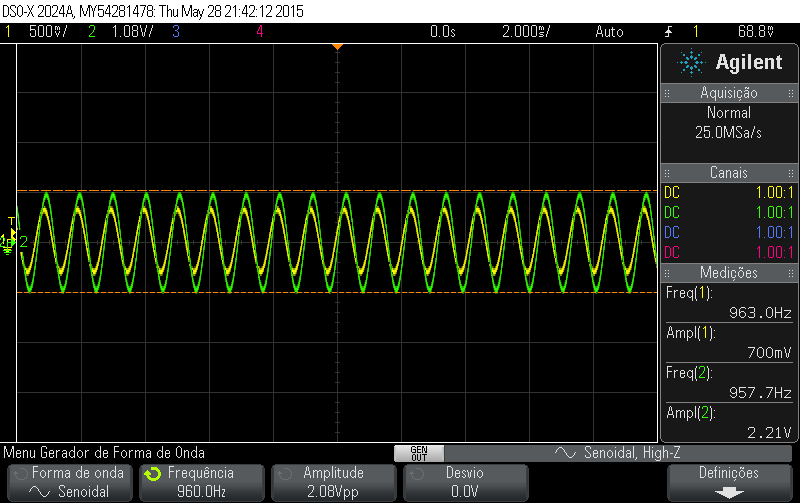
\includegraphics[keepaspectratio=true, scale=0.37]{exps/filtro_1k_freqcorte}
	\caption{Verificação da frequência de corte - sinal de entrada (a verde) e sinal de saída (a amarelo) do filtro \textit{data}.}
	\vspace{-0.8em}
\end{figure} 



\todo{4 - nao nos lembramos do que era isto}

\todo{5 - margarida}

Com o \textit{Costas Loop} implementado pretende-se testar o seu funcionamento para um sinal de entrada sinusoidal. Numa primeira fase de testes apenas se considera o \textit{upper arm}, de maneira a que o \textit{loop} se comporte como um clássico DPLL (\textit{digital phase locked loop}), tal como se pode observar na figura abaixo. Um DPLL é um tipo de PLL que é realizado com recurso a circuitos lógicos e/ou microprocessadores, tendo a capacidade de processar sinais discretos tanto em tempo como em amplitude.

\begin{figure}[H]
	\centering
	\subfloat[]{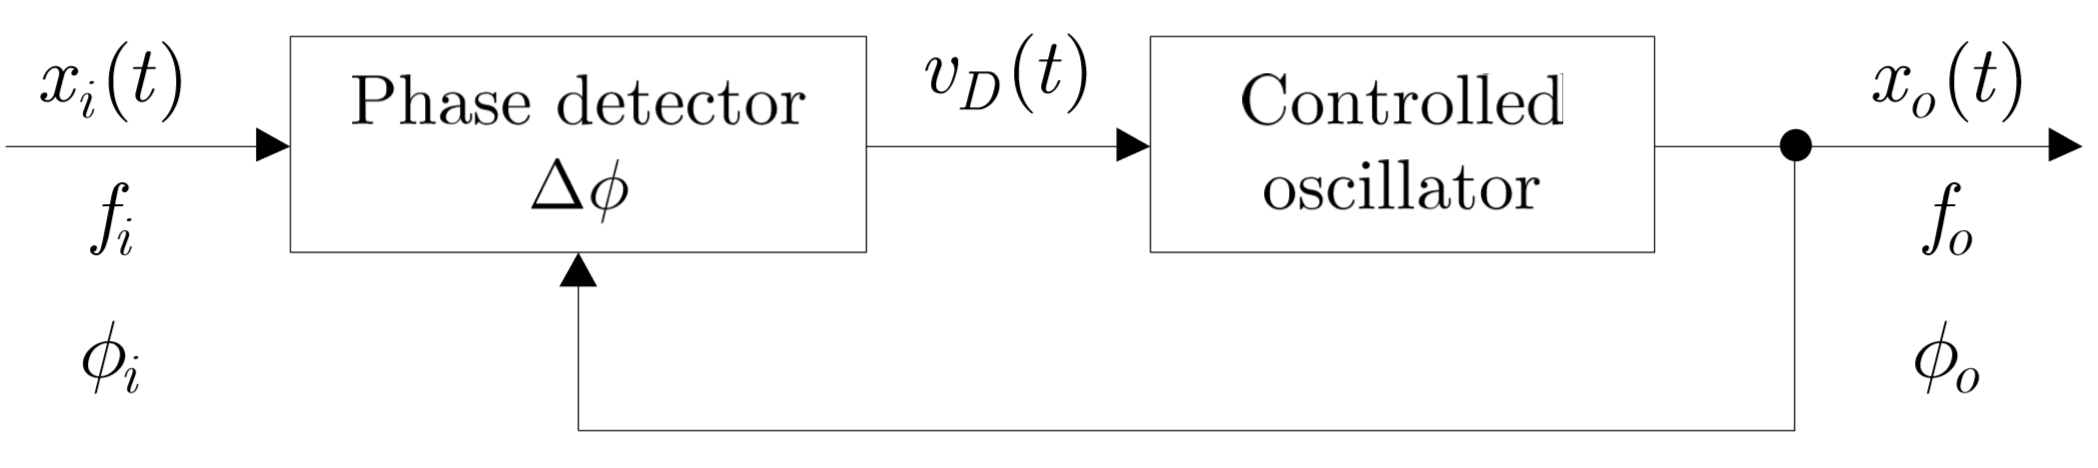
\includegraphics[keepaspectratio=true, scale=0.284]{teoricas/pll}}
	\hspace{8mm}
	\subfloat[]{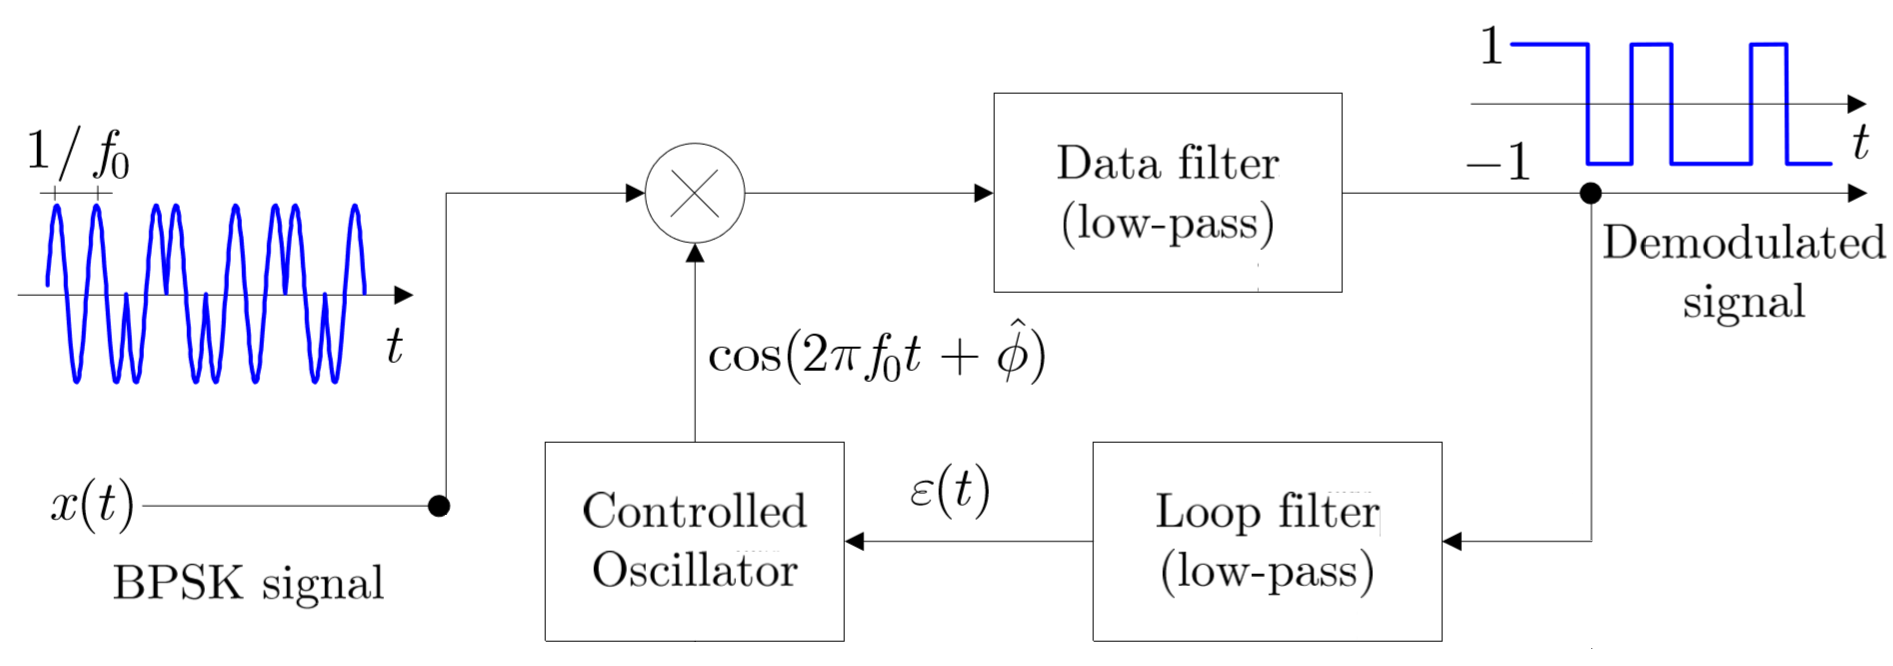
\includegraphics[keepaspectratio=true, scale=0.284]{teoricas/dpll}}
	\vspace{-0.8em}
	\caption{Diagrama de blocos de um PLL básico (a) e do \textit{upper arm} do \textit{Costas Loop} projectado (b).}
	\vspace{-0.8em}
\end{figure}

As duas fases $\phi_{i}$ e $\phi_{o}$ são comparadas no detector de fase, o que gera o sinal $v_{D}\left(t\right)$ que é uma função da diferença $\phi_{i} - \phi_{o}$ (sinal de erro). Este sinal controla a frequência (e, consequentemente, a fase) do oscilador de maneira a que $\phi_{o}$ ``segue'' a variação em $\phi_{i}$.

Posto isto, o PLL pode estar num de dois estados - \textit{locked} (sincronizado) ou \textit{unlocked} (dessincronizado). Quando no primeiro estado o oscilador gera um sinal com uma frequência que é, em média, igual à frequência do sinal de entrada $f_o = f_i$ e o \textit{loop} ajusta o oscilador de fase de modo a que este ``siga'' $\phi_{i}$. Quando o PLL se encontra no segundo estado, a frequência $f_o$ não está relacionada com $f_i$ e se houver variações em $\phi_{i}$ estas não serão necessariamente ``seguidas'' por $\phi_{o}$.

Assim, para testar o correcto funcionamento do PLL projectado é necessário verificar o comportamento do sinal à saída do oscilador controlado e à entrada do detector de fase. No projecto em causa o detector de fase é um multiplicador, que é o adequado para processar sinais do tipo sinusoidal. 

À entrada colocou-se um sinal sinusoidal com amplitude de 1 $V_{PP}$, fazendo-se variar a sua frequência, partindo de um valor inicial de 4 kHz que é a frequência de funcionamento da malha dessincronizada. Nas figuras seguintes apresenta-se o comportamento do PLL para duas situações distintas, estando representado a amarelo o sinal de entrada e a verde o sinal à saída do oscilador controlado.

\begin{figure}[H]
	\centering
	\subfloat[]{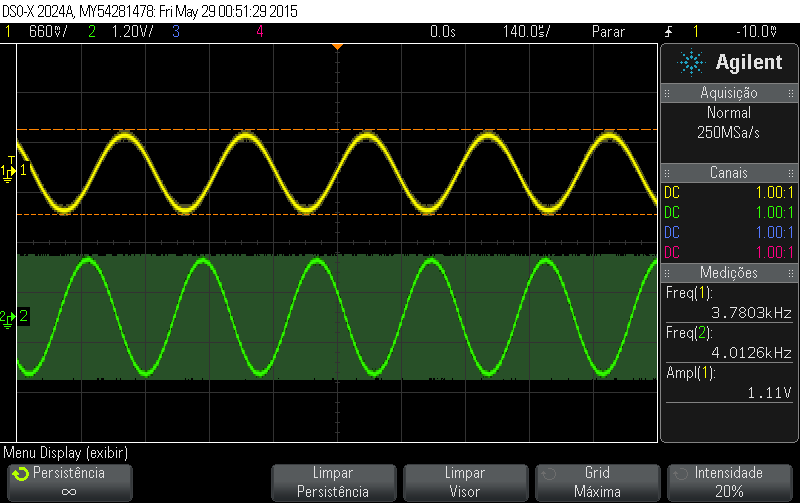
\includegraphics[keepaspectratio=true, scale=0.284]{exps/upperarm_desync}}
	\hspace{8mm}
	\subfloat[]{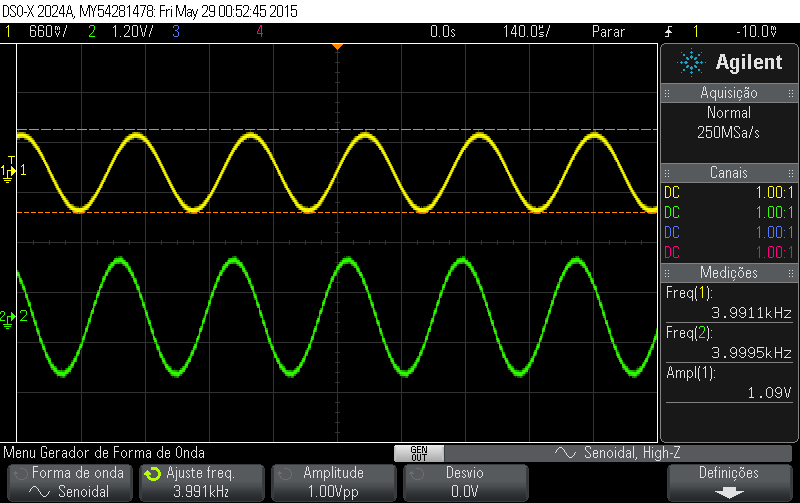
\includegraphics[keepaspectratio=true, scale=0.284]{exps/upperarm_sync}}
	\vspace{-0.8em}
	\caption{Situação em que o PLL está dessincronizado (a) e sincronizado (b).}
	\label{fig:PLL}
	\vspace{-0.8em}
\end{figure}

Para ambas as situações recorreu-se ao modo persistência do osciloscópio, com o objectivo de ajudar a reconhecer a situação de dessincronismo do PLL. De facto, na Figura \ref{fig:PLL}(a) verifica-se que o sinal â saída do oscilador apresenta bastante dispersão em torno dos valores pretendidos para a forma de onda, tal como esperado. Quando se ajustou a frequência do sinal de entrada e o PLL entrou num estado de sincronismo obtém-se os resultados da Figura \ref{fig:PLL}(b), em que o sinal representado a verde não apresenta dispersão em torno dos valores pretendidos, tal como esperado.

Uma vez verificado o correcto funcionamento do \textit{upper arm} do \textit{Costas Loop}, conectou-se o \textit{lower arm} e testou-se todo o \textit{loop} utilizando também um sinal sinusoidal à entrada. Verificou-se que ambos os \textit{arms} apresentam o comportamento esperado. Assim, procede-se à medição da banda de captura e da banda de manutenção do \textit{loop}.

O sinal de entrada deve estar compreendido na banda de captura do \textit{loop}. Uma vez que se adquira o sincronismo, o \textit{loop} manter-se-á nesse estado, dentro de certos limites, que definem a banda de manutenção, sendo que esta banda pode ser diferente da banda de captura. 

Para se calcular experimentalmente o valor das bandas é necessário observar o valor médio do sinal de erro, enquanto se faz variar lentamente a frequência do sinal de entrada decrescentemente, partindo de um estado inicial de \textit{loop} dessincronizado, até que ocorre uma captura em $w_{C}^{-}$. De seguida aumenta-se a frequência do sinal de entrada até que se perde o sincronismo em $w_{L}^{+}$. O passo seguinte é efectuar um varrimento no sentido contrário, adquirindo sincronismo em $w_{C}^{+}$ que depois é perdido em $w_{L}^{-}$.

Relativamente ao sinal de erro que se observa nesta medição, considere-se o caso em que o PLL está fora de sincronismo e o oscilador gera uma frequência $f_o$. Quando o \textit{loop} se fecha (ou quando o sinal de entrada tem uma frequência $f_i$) se a diferença entre as duas frequências for pequena o suficiente, então o filtro de  \textit{loop} irá desenvolver um sinal de erro que leva a frequência do oscilador até $f_i$. Eventualmente o \textit{loop} vai adquirir sincronismo e neste estado a frequência média gerada pelo oscilador é igual à frequência média do sinal de entrada.

\begin{figure}[H]
	\centering
	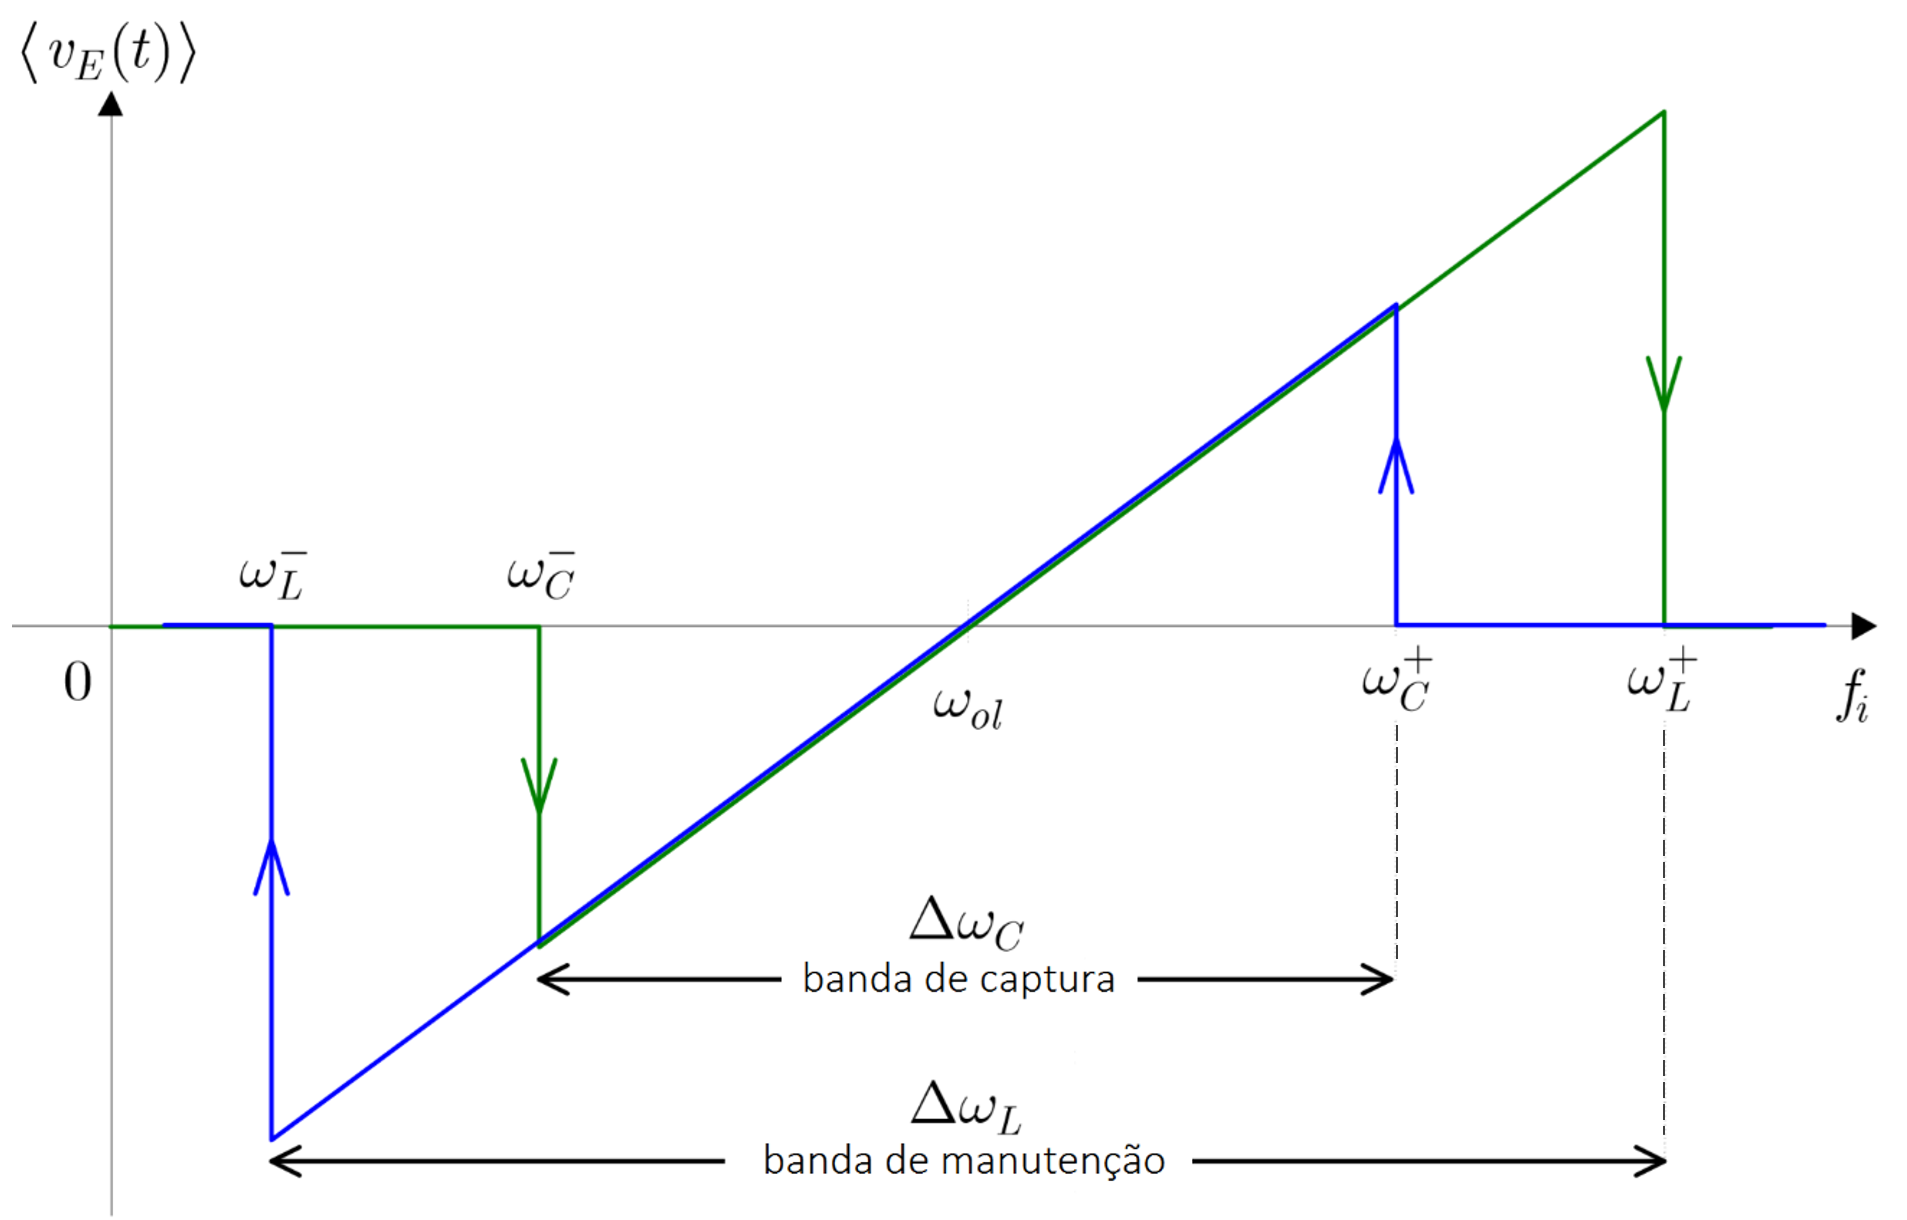
\includegraphics[keepaspectratio=true, scale=0.25]{teoricas/malhas}
	\caption{Representação das bandas que caracterizam o PLL.}
	\vspace{-0.8em}
\end{figure} 

Da figura anterior verifica-se que, regra geral, $\Delta w_L \geq \Delta w_C$.

\todo{continuar bandas}

O passo seguinte corresponde à conexão entre o modulador do transmissor e o desmodulador do receptor, ou seja, o sinal de entrada do \textit{Costas Loop} é o sinal modelado do tipo BPSK. Este sinal corresponde à multiplicação do sinal $d_n$ com a portadora, como se viu já anteriormente.

\todo{depois desta parte comentamos as imagens que tiramos no ultimo lab}

\todo{Parte do filtro de 8 k}

Realizando o teste do filtro \textit{Data} com uma entrada sinusoidal de 8 kHz, é possível, observando a Figura X, perceber que o filtro não anula completamente o sinal de entrada, o que causa o problema descrito acima. 

\begin{figure}[H]
	\centering
	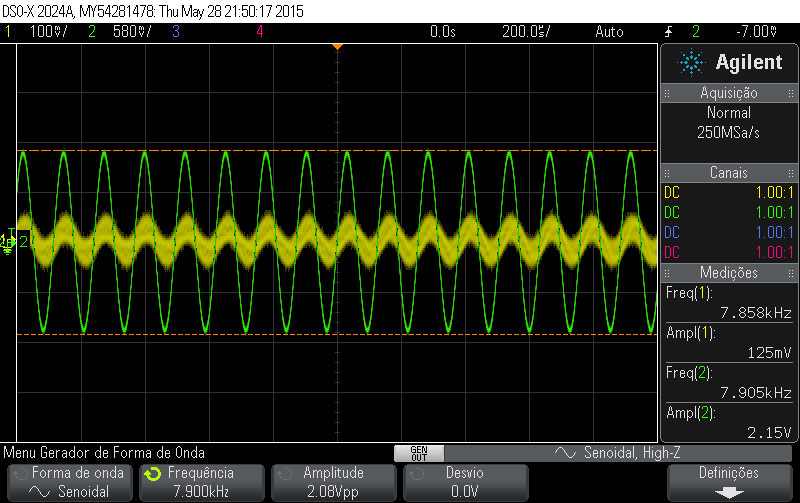
\includegraphics[keepaspectratio=true, scale=0.50]{exps/FiltroSemZero8k}
	\caption{Sinal de entrada(verde) e sinal de saída(amarelo) do filtro \textit{Data}}
	\label{fig:fluxo}
	\vspace{-0.8em}
\end{figure} 

De forma a solucionar este problema, implementou-se um filtro idêntico ao já implementado, adicionando um zero na frequência de 8 kHz, o que permite anular essa componente no sinal de saída. Assim, de forma a implementar esta solução, é necessário que $\beta = -1$, que vem de:

\vspace{-3mm}
\begin{equation}
H(z) = \frac{\gamma \frac{1-\alpha}{1-\beta} (1-\beta z^{-1})}{1-\alpha z^{-1}} = 0 \Rightarrow \beta z = 1.
\end{equation}


e, para a frequência de 8 kHz, sendo $z = e^{j\omega T_s} = e^{j2\pi \frac{8\times 10^3}{16\times 10^3}}$, é possível determinar o valor de $\beta$.
	
Resulta então a função de transferência, mantendo-se os valores de $\alpha e \gamma$:

\vspace{-3mm}
\begin{equation}
H(z) = \frac{\gamma \frac{1-\alpha}{2} (1+z^{-1})}{1-\alpha z^{-1}}
\end{equation}

concluindo-se que, em relação à implementação anterior, basta dividir o ganho por 2 e utilizar o valor da amostra anterior, somando-a à actual, respeitando a seguinte equação às diferenças:

\vspace{-3mm}
\begin{equation}
y(n) = \alpha y(n-1) +  (1-\alpha)[x(n) + x(n-1)]
\end{equation} 

cujo excerto de código que permite implementar essa equação é apresentado de seguida.

\begin{lstlisting}[language=C]
short x_cos = 0, x_sine = 0, y_cos_datafilter = 0, y_sin_datafilter = 0;  
short in_loopfilter = 0, y_loop filter = 0, alpha_1k = 23528; 
short alpha_10 = 32640, um_menos_alpha_1k = 9240, um_menos_alpha_10 = 127;
...
 //Data filter com zero em ws/2
 y_cos_datafilter = (((alpha_1k*y_cos_datafilter)<<1) + ((((x_cos + x_cos_old)*um_menos_alpha_1k)>>1)<<1))>>16;
 y_sin_datafilter = (((alpha_1k*y_sin_datafilter)<<1) + ((((x_sine + x_sine_old)*um_menos_alpha_1k)>>1)<<1))>>16;

 x_cos_old = x_cos;
 x_sine_old = x_sin;

...

\end{lstlisting}

Na Figura X, pode observar-se a saída do filtro digital implementado com um zero em 8 kHz, para um sinal de entrada sinusoidal com essa frequência. 

\begin{figure}[H]
	\centering
	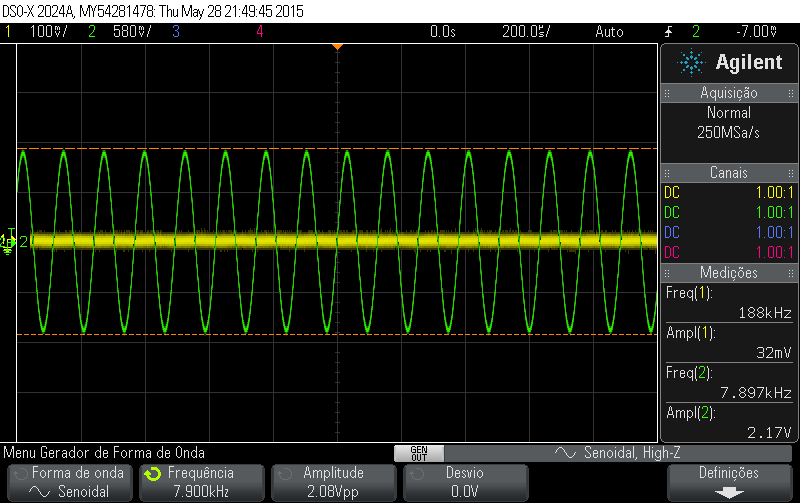
\includegraphics[keepaspectratio=true, scale=0.50]{exps/FiltroComZero8k}
	\caption{Sinal de entrada(verde) e sinal de saída(amarelo) do filtro \textit{Data}}
	\label{fig:fluxo}
	\vspace{-0.8em}
\end{figure} 

Conclui-se assim que o filtro implementado anula a componente de 8 kHz, o que comprova a implementação de forma correcta do mesmo, permitindo que o sinal de saída do filtro, com o \textit{Costas Loop} completo, apresente de uma forma clara uma diferença entre o nível \textit{high} e \textit{low}, tal como representado na Figura X.

\begin{figure}[H]
	\centering
	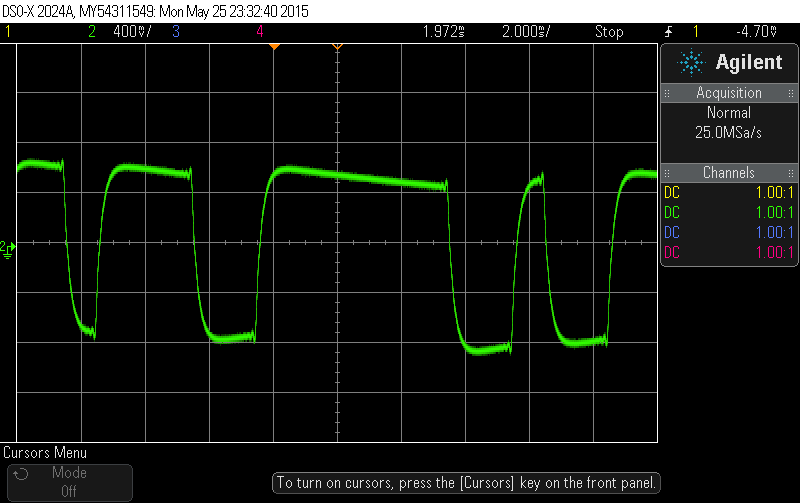
\includegraphics[keepaspectratio=true, scale=0.50]{exps/pulse_saida_filtro_Sine_mudancanoFiltro}
	\caption{Sinal à saída do filtro \textit{Data} com \textit{Costas Loop} completo}
	\label{fig:fluxo}
	\vspace{-0.8em}
\end{figure}

\section{Conclusões}

Relativamente ao Projecto \#1, pode-se concluir que um oscilador controlado feito com recurso ao método da interpolação apresenta resultados com mais qualidade, isto para casos em que o valor de $\Delta$ representa frequências que não são múltiplos da frequência de amostragem. 

Já em relação ao Projecto \#2, este correu de acordo com o esperado, sendo que se procedeu a uma melhoria ao nível da eficiência do código para que apenas houvesse o \textit{if} do contador. Verificou-se que retirar este último \textit{if} não compensava pois era necessário replicar o código e a eficiência computacional seria equiparável. 

\pagebreak

\section{Anexos}

\subsection{Anexo I - Código do Projecto \#1}

\begin{lstlisting}[language=C]
#include "dsk6713_aic23.h"
#include "C6713dskinit.h"

Uint32 fs = DSK6713_AIC23_FREQ_16KHZ;

char	intflag = FALSE;
union	{Uint32 samples; short channel[2];} AIC_buffer;

short sine[33] = {0,3212,6393,9512,12540,15447,18205,20788,23170,25330,27246,28899,30274,31357,		32138,32610,32767,32610,32138,31357,30274,28899,27246,25330,23170,20788,18205,	15447,12540,9512,6393,3212,0}; 

interrupt void c_int11(){                  	
	output_sample(AIC_buffer.samples); 
	AIC_buffer.samples= input_sample(); 
	intflag = TRUE;
	return;
}

void main(){
	short	inbuf = 0;
	short	delta = 0 ;
	short	status = -32767;
	short	y1 = 0, y2 = 0, y_n = 0, y_s = 0;
	short	i = 0, delta_x = 0;
	short	amp = 16384;
	
	comm_intr();
	while(1){
		if(intflag != FALSE){
			intflag = FALSE;
				
			inbuf = AIC_buffer.channel[LEFT];
			
			delta = 16384 + (inbuf>>2);
			
			status = status + delta;
			delta_x = (status & 1023)<<5;
			
			i = (status>>10)&31;
			y1 = sine[i];
			y2 = sine[i+1];
			y_s = amp*(y1 + delta)>>15;  
			y_n = (amp*(y1 + ((y2-y1)*delta_x>>15))>>15);
			
			if(status < 0){
				y_s = -y_s;
				y_n = -y_n;
			}
			AIC_buffer.channel[LEFT] = y_n;  //saida com interpolacao
			AIC_buffer.channel[RIGHT] = y_s; //saida sem interpolacao
		}
	}
}
\end{lstlisting}

\subsection{Anexo II - Código do Projecto \#2}

\begin{lstlisting}[language=C]
#include "dsk6713_aic23.h"	
#include "C6713dskinit.h"

Uint32 fs = DSK6713_AIC23_FREQ_16KHZ;	

char	intflag = FALSE;
union	{Uint32 samples; short channel[2];} AIC_buffer;

short	sine[4] = {0,32767,0,-32767};

interrupt void c_int11(){
	output_sample(AIC_buffer.samples);   	
	AIC_buffer.samples= input_sample(); 	    
	intflag = TRUE;
	return;
}

void main(){
	short	d_n, y;
	short	b_i = 1, sine_i = 0, b = 0;
	short	c_n = 0;
	short	b_n = 1, shift15_cn = 0, not_shift15 = 0;
	
	comm_intr();
	while(1){
		if(intflag != FALSE){
			intflag = FALSE;
			
			sine_i= sine_i&3;
			y = sine[sine_i];
			sine_i++;
			y = (32767*y)>>15 ; //esta linha e para tirar?
			
			
			/* implementacao do contador sem recurso a instruccao condicional if */
				//b_i++;
				//b=(b_i&16)>>4;
				//b_n=(b_n^b);
				//b_i=(b_i&15);*/
			if(b_i>15){
				b_i=0;
				b_n=(b_n^1);
				c_n=c_n^b_n;
				shift15_cn=c_n<<15;
				not_shift15=~shift15_cn;
				d_n=not_shift15>>14;				
			}
			b_i++;
			y=d_n*y;
			
			AIC_buffer.channel[LEFT] = y;
		}
	}
}
\end{lstlisting}

\end{document}